\documentclass[twoside]{book}

% Packages required by doxygen
\usepackage{fixltx2e}
\usepackage{calc}
\usepackage{doxygen}
\usepackage[export]{adjustbox} % also loads graphicx
\usepackage{graphicx}
\usepackage[utf8]{inputenc}
\usepackage{makeidx}
\usepackage{multicol}
\usepackage{multirow}
\PassOptionsToPackage{warn}{textcomp}
\usepackage{textcomp}
\usepackage[nointegrals]{wasysym}
\usepackage[table]{xcolor}

% Font selection
\usepackage[T1]{fontenc}
\usepackage[scaled=.90]{helvet}
\usepackage{courier}
\usepackage{amssymb}
\usepackage{sectsty}
\renewcommand{\familydefault}{\sfdefault}
\allsectionsfont{%
  \fontseries{bc}\selectfont%
  \color{darkgray}%
}
\renewcommand{\DoxyLabelFont}{%
  \fontseries{bc}\selectfont%
  \color{darkgray}%
}
\newcommand{\+}{\discretionary{\mbox{\scriptsize$\hookleftarrow$}}{}{}}

% Page & text layout
\usepackage{geometry}
\geometry{%
  a4paper,%
  top=2.5cm,%
  bottom=2.5cm,%
  left=2.5cm,%
  right=2.5cm%
}
\tolerance=750
\hfuzz=15pt
\hbadness=750
\setlength{\emergencystretch}{15pt}
\setlength{\parindent}{0cm}
\setlength{\parskip}{3ex plus 2ex minus 2ex}
\makeatletter
\renewcommand{\paragraph}{%
  \@startsection{paragraph}{4}{0ex}{-1.0ex}{1.0ex}{%
    \normalfont\normalsize\bfseries\SS@parafont%
  }%
}
\renewcommand{\subparagraph}{%
  \@startsection{subparagraph}{5}{0ex}{-1.0ex}{1.0ex}{%
    \normalfont\normalsize\bfseries\SS@subparafont%
  }%
}
\makeatother

% Headers & footers
\usepackage{fancyhdr}
\pagestyle{fancyplain}
\fancyhead[LE]{\fancyplain{}{\bfseries\thepage}}
\fancyhead[CE]{\fancyplain{}{}}
\fancyhead[RE]{\fancyplain{}{\bfseries\leftmark}}
\fancyhead[LO]{\fancyplain{}{\bfseries\rightmark}}
\fancyhead[CO]{\fancyplain{}{}}
\fancyhead[RO]{\fancyplain{}{\bfseries\thepage}}
\fancyfoot[LE]{\fancyplain{}{}}
\fancyfoot[CE]{\fancyplain{}{}}
\fancyfoot[RE]{\fancyplain{}{\bfseries\scriptsize Generated by Doxygen }}
\fancyfoot[LO]{\fancyplain{}{\bfseries\scriptsize Generated by Doxygen }}
\fancyfoot[CO]{\fancyplain{}{}}
\fancyfoot[RO]{\fancyplain{}{}}
\renewcommand{\footrulewidth}{0.4pt}
\renewcommand{\chaptermark}[1]{%
  \markboth{#1}{}%
}
\renewcommand{\sectionmark}[1]{%
  \markright{\thesection\ #1}%
}

% Indices & bibliography
\usepackage{natbib}
\usepackage[titles]{tocloft}
\setcounter{tocdepth}{3}
\setcounter{secnumdepth}{5}
\makeindex

% Hyperlinks (required, but should be loaded last)
\usepackage{ifpdf}
\ifpdf
  \usepackage[pdftex,pagebackref=true]{hyperref}
\else
  \usepackage[ps2pdf,pagebackref=true]{hyperref}
\fi
\hypersetup{%
  colorlinks=true,%
  linkcolor=blue,%
  citecolor=blue,%
  unicode%
}

% Custom commands
\newcommand{\clearemptydoublepage}{%
  \newpage{\pagestyle{empty}\cleardoublepage}%
}

\usepackage{caption}
\captionsetup{labelsep=space,justification=centering,font={bf},singlelinecheck=off,skip=4pt,position=top}

%===== C O N T E N T S =====

\begin{document}

% Titlepage & ToC
\hypersetup{pageanchor=false,
             bookmarksnumbered=true,
             pdfencoding=unicode
            }
\pagenumbering{alph}
\begin{titlepage}
\vspace*{7cm}
\begin{center}%
{\Large Deusto Newspaper }\\
\vspace*{1cm}
{\large Generated by Doxygen 1.8.13}\\
\end{center}
\end{titlepage}
\clearemptydoublepage
\pagenumbering{roman}
\tableofcontents
\clearemptydoublepage
\pagenumbering{arabic}
\hypersetup{pageanchor=true}

%--- Begin generated contents ---
\chapter{Namespace Index}
\section{Packages}
Here are the packages with brief descriptions (if available)\+:\begin{DoxyCompactList}
\item\contentsline{section}{\hyperlink{namespacees}{es} }{\pageref{namespacees}}{}
\item\contentsline{section}{\hyperlink{namespacees_1_1deusto}{es.\+deusto} }{\pageref{namespacees_1_1deusto}}{}
\item\contentsline{section}{\hyperlink{namespacees_1_1deusto_1_1client}{es.\+deusto.\+client} \\*This is the brief documentation for the Java package \hyperlink{namespacees_1_1deusto_1_1client}{es.\+deusto.\+client} which is a package for the client logic }{\pageref{namespacees_1_1deusto_1_1client}}{}
\item\contentsline{section}{\hyperlink{namespacees_1_1deusto_1_1client_1_1_g_u_i}{es.\+deusto.\+client.\+G\+UI} \\*This is the brief documentation for the Java package \hyperlink{namespacees_1_1deusto_1_1client_1_1_g_u_i}{es.\+deusto.\+client.\+G\+UI} which is a package for the client \hyperlink{namespacees_1_1deusto_1_1client_1_1_g_u_i}{G\+UI} }{\pageref{namespacees_1_1deusto_1_1client_1_1_g_u_i}}{}
\item\contentsline{section}{\hyperlink{namespacees_1_1deusto_1_1server}{es.\+deusto.\+server} \\*This is the brief documentation for the Java package \hyperlink{namespacees_1_1deusto_1_1server}{es.\+deusto.\+server} which is a package for the logic of the server }{\pageref{namespacees_1_1deusto_1_1server}}{}
\item\contentsline{section}{\hyperlink{namespacees_1_1deusto_1_1server_1_1jdo}{es.\+deusto.\+server.\+jdo} }{\pageref{namespacees_1_1deusto_1_1server_1_1jdo}}{}
\end{DoxyCompactList}

\chapter{Hierarchical Index}
\section{Class Hierarchy}
This inheritance list is sorted roughly, but not completely, alphabetically\+:\begin{DoxyCompactList}
\item \contentsline{section}{es.\+deusto.\+server.\+jdo.\+Admin\+Test}{\pageref{classes_1_1deusto_1_1server_1_1jdo_1_1_admin_test}}{}
\item \contentsline{section}{es.\+deusto.\+server.\+jdo.\+Article\+Test}{\pageref{classes_1_1deusto_1_1server_1_1jdo_1_1_article_test}}{}
\item \contentsline{section}{es.\+deusto.\+client.\+Client}{\pageref{classes_1_1deusto_1_1client_1_1_client}}{}
\item \contentsline{section}{es.\+deusto.\+server.\+jdo.\+D\+B\+Test}{\pageref{classes_1_1deusto_1_1server_1_1jdo_1_1_d_b_test}}{}
\item \contentsline{section}{es.\+deusto.\+server.\+Server\+Test}{\pageref{classes_1_1deusto_1_1server_1_1_server_test}}{}
\item \contentsline{section}{es.\+deusto.\+server.\+jdo.\+User\+Test}{\pageref{classes_1_1deusto_1_1server_1_1jdo_1_1_user_test}}{}
\item J\+Frame\begin{DoxyCompactList}
\item \contentsline{section}{es.\+deusto.\+client.\+G\+U\+I.\+Article\+Window}{\pageref{classes_1_1deusto_1_1client_1_1_g_u_i_1_1_article_window}}{}
\item \contentsline{section}{es.\+deusto.\+client.\+G\+U\+I.\+Login\+Window\+User}{\pageref{classes_1_1deusto_1_1client_1_1_g_u_i_1_1_login_window_user}}{}
\item \contentsline{section}{es.\+deusto.\+client.\+G\+U\+I.\+Main\+Window}{\pageref{classes_1_1deusto_1_1client_1_1_g_u_i_1_1_main_window}}{}
\end{DoxyCompactList}
\item Remote\begin{DoxyCompactList}
\item \contentsline{section}{es.\+deusto.\+server.\+I\+Server}{\pageref{interfacees_1_1deusto_1_1server_1_1_i_server}}{}
\begin{DoxyCompactList}
\item \contentsline{section}{es.\+deusto.\+server.\+Server}{\pageref{classes_1_1deusto_1_1server_1_1_server}}{}
\end{DoxyCompactList}
\end{DoxyCompactList}
\item Serializable\begin{DoxyCompactList}
\item \contentsline{section}{es.\+deusto.\+server.\+jdo.\+Article}{\pageref{classes_1_1deusto_1_1server_1_1jdo_1_1_article}}{}
\item \contentsline{section}{es.\+deusto.\+server.\+jdo.\+User}{\pageref{classes_1_1deusto_1_1server_1_1jdo_1_1_user}}{}
\begin{DoxyCompactList}
\item \contentsline{section}{es.\+deusto.\+server.\+jdo.\+Admin}{\pageref{classes_1_1deusto_1_1server_1_1jdo_1_1_admin}}{}
\end{DoxyCompactList}
\end{DoxyCompactList}
\item Test\+Case\begin{DoxyCompactList}
\item \contentsline{section}{es.\+deusto.\+client.\+Client\+Test}{\pageref{classes_1_1deusto_1_1client_1_1_client_test}}{}
\end{DoxyCompactList}
\item Unicast\+Remote\+Object\begin{DoxyCompactList}
\item \contentsline{section}{es.\+deusto.\+server.\+Server}{\pageref{classes_1_1deusto_1_1server_1_1_server}}{}
\end{DoxyCompactList}
\end{DoxyCompactList}

\chapter{Class Index}
\section{Class List}
Here are the classes, structs, unions and interfaces with brief descriptions\+:\begin{DoxyCompactList}
\item\contentsline{section}{\hyperlink{classes_1_1deusto_1_1server_1_1jdo_1_1_admin}{es.\+deusto.\+server.\+jdo.\+Admin} }{\pageref{classes_1_1deusto_1_1server_1_1jdo_1_1_admin}}{}
\item\contentsline{section}{\hyperlink{classes_1_1deusto_1_1server_1_1jdo_1_1_admin_test}{es.\+deusto.\+server.\+jdo.\+Admin\+Test} }{\pageref{classes_1_1deusto_1_1server_1_1jdo_1_1_admin_test}}{}
\item\contentsline{section}{\hyperlink{classes_1_1deusto_1_1server_1_1jdo_1_1_article}{es.\+deusto.\+server.\+jdo.\+Article} }{\pageref{classes_1_1deusto_1_1server_1_1jdo_1_1_article}}{}
\item\contentsline{section}{\hyperlink{classes_1_1deusto_1_1server_1_1jdo_1_1_article_test}{es.\+deusto.\+server.\+jdo.\+Article\+Test} }{\pageref{classes_1_1deusto_1_1server_1_1jdo_1_1_article_test}}{}
\item\contentsline{section}{\hyperlink{classes_1_1deusto_1_1client_1_1_g_u_i_1_1_article_window}{es.\+deusto.\+client.\+G\+U\+I.\+Article\+Window} }{\pageref{classes_1_1deusto_1_1client_1_1_g_u_i_1_1_article_window}}{}
\item\contentsline{section}{\hyperlink{classes_1_1deusto_1_1client_1_1_client}{es.\+deusto.\+client.\+Client} }{\pageref{classes_1_1deusto_1_1client_1_1_client}}{}
\item\contentsline{section}{\hyperlink{classes_1_1deusto_1_1client_1_1_client_test}{es.\+deusto.\+client.\+Client\+Test} }{\pageref{classes_1_1deusto_1_1client_1_1_client_test}}{}
\item\contentsline{section}{\hyperlink{classes_1_1deusto_1_1server_1_1jdo_1_1_d_b_test}{es.\+deusto.\+server.\+jdo.\+D\+B\+Test} }{\pageref{classes_1_1deusto_1_1server_1_1jdo_1_1_d_b_test}}{}
\item\contentsline{section}{\hyperlink{interfacees_1_1deusto_1_1server_1_1_i_server}{es.\+deusto.\+server.\+I\+Server} }{\pageref{interfacees_1_1deusto_1_1server_1_1_i_server}}{}
\item\contentsline{section}{\hyperlink{classes_1_1deusto_1_1client_1_1_g_u_i_1_1_login_window_user}{es.\+deusto.\+client.\+G\+U\+I.\+Login\+Window\+User} }{\pageref{classes_1_1deusto_1_1client_1_1_g_u_i_1_1_login_window_user}}{}
\item\contentsline{section}{\hyperlink{classes_1_1deusto_1_1client_1_1_g_u_i_1_1_main_window}{es.\+deusto.\+client.\+G\+U\+I.\+Main\+Window} }{\pageref{classes_1_1deusto_1_1client_1_1_g_u_i_1_1_main_window}}{}
\item\contentsline{section}{\hyperlink{classes_1_1deusto_1_1server_1_1_server}{es.\+deusto.\+server.\+Server} }{\pageref{classes_1_1deusto_1_1server_1_1_server}}{}
\item\contentsline{section}{\hyperlink{classes_1_1deusto_1_1server_1_1_server_test}{es.\+deusto.\+server.\+Server\+Test} }{\pageref{classes_1_1deusto_1_1server_1_1_server_test}}{}
\item\contentsline{section}{\hyperlink{classes_1_1deusto_1_1server_1_1jdo_1_1_user}{es.\+deusto.\+server.\+jdo.\+User} }{\pageref{classes_1_1deusto_1_1server_1_1jdo_1_1_user}}{}
\item\contentsline{section}{\hyperlink{classes_1_1deusto_1_1server_1_1jdo_1_1_user_test}{es.\+deusto.\+server.\+jdo.\+User\+Test} }{\pageref{classes_1_1deusto_1_1server_1_1jdo_1_1_user_test}}{}
\end{DoxyCompactList}

\chapter{File Index}
\section{File List}
Here is a list of all files with brief descriptions\+:\begin{DoxyCompactList}
\item\contentsline{section}{src/main/java/es/deusto/client/\hyperlink{_client_8java}{Client.\+java} }{\pageref{_client_8java}}{}
\item\contentsline{section}{src/main/java/es/deusto/client/\+G\+U\+I/\hyperlink{_article_window_8java}{Article\+Window.\+java} }{\pageref{_article_window_8java}}{}
\item\contentsline{section}{src/main/java/es/deusto/client/\+G\+U\+I/\hyperlink{_login_window_user_8java}{Login\+Window\+User.\+java} }{\pageref{_login_window_user_8java}}{}
\item\contentsline{section}{src/main/java/es/deusto/client/\+G\+U\+I/\hyperlink{_main_window_8java}{Main\+Window.\+java} }{\pageref{_main_window_8java}}{}
\item\contentsline{section}{src/main/java/es/deusto/server/\hyperlink{_i_server_8java}{I\+Server.\+java} }{\pageref{_i_server_8java}}{}
\item\contentsline{section}{src/main/java/es/deusto/server/\hyperlink{_server_8java}{Server.\+java} }{\pageref{_server_8java}}{}
\item\contentsline{section}{src/main/java/es/deusto/server/jdo/\hyperlink{_admin_8java}{Admin.\+java} }{\pageref{_admin_8java}}{}
\item\contentsline{section}{src/main/java/es/deusto/server/jdo/\hyperlink{_article_8java}{Article.\+java} }{\pageref{_article_8java}}{}
\item\contentsline{section}{src/main/java/es/deusto/server/jdo/\hyperlink{_d_b_test_8java}{D\+B\+Test.\+java} }{\pageref{_d_b_test_8java}}{}
\item\contentsline{section}{src/main/java/es/deusto/server/jdo/\hyperlink{_user_8java}{User.\+java} }{\pageref{_user_8java}}{}
\item\contentsline{section}{src/test/java/\hyperlink{_r_m_i_test_8java}{R\+M\+I\+Test.\+java} }{\pageref{_r_m_i_test_8java}}{}
\item\contentsline{section}{src/test/java/es/deusto/client/\hyperlink{_client_test_8java}{Client\+Test.\+java} }{\pageref{_client_test_8java}}{}
\item\contentsline{section}{src/test/java/es/deusto/server/\hyperlink{_server_test_8java}{Server\+Test.\+java} }{\pageref{_server_test_8java}}{}
\item\contentsline{section}{src/test/java/es/deusto/server/jdo/\hyperlink{_admin_test_8java}{Admin\+Test.\+java} }{\pageref{_admin_test_8java}}{}
\item\contentsline{section}{src/test/java/es/deusto/server/jdo/\hyperlink{_article_test_8java}{Article\+Test.\+java} }{\pageref{_article_test_8java}}{}
\item\contentsline{section}{src/test/java/es/deusto/server/jdo/\hyperlink{_user_test_8java}{User\+Test.\+java} }{\pageref{_user_test_8java}}{}
\end{DoxyCompactList}

\chapter{Namespace Documentation}
\hypertarget{namespacees}{}\section{Package es}
\label{namespacees}\index{es@{es}}
\subsection*{Packages}
\begin{DoxyCompactItemize}
\item 
package \hyperlink{namespacees_1_1deusto}{deusto}
\end{DoxyCompactItemize}

\hypertarget{namespacees_1_1deusto}{}\section{Package es.\+deusto}
\label{namespacees_1_1deusto}\index{es.\+deusto@{es.\+deusto}}
\subsection*{Packages}
\begin{DoxyCompactItemize}
\item 
package \hyperlink{namespacees_1_1deusto_1_1client}{client}
\item 
package \hyperlink{namespacees_1_1deusto_1_1server}{server}
\end{DoxyCompactItemize}

\hypertarget{namespacees_1_1deusto_1_1client}{}\section{Package es.\+deusto.\+client}
\label{namespacees_1_1deusto_1_1client}\index{es.\+deusto.\+client@{es.\+deusto.\+client}}
\subsection*{Packages}
\begin{DoxyCompactItemize}
\item 
package \hyperlink{namespacees_1_1deusto_1_1client_1_1_g_u_i}{G\+UI}
\end{DoxyCompactItemize}
\subsection*{Classes}
\begin{DoxyCompactItemize}
\item 
class \hyperlink{classes_1_1deusto_1_1client_1_1_client}{Client}
\item 
class \hyperlink{classes_1_1deusto_1_1client_1_1_client_test}{Client\+Test}
\end{DoxyCompactItemize}

\hypertarget{namespacees_1_1deusto_1_1client_1_1_g_u_i}{}\section{Package es.\+deusto.\+client.\+G\+UI}
\label{namespacees_1_1deusto_1_1client_1_1_g_u_i}\index{es.\+deusto.\+client.\+G\+UI@{es.\+deusto.\+client.\+G\+UI}}
\subsection*{Classes}
\begin{DoxyCompactItemize}
\item 
class \hyperlink{classes_1_1deusto_1_1client_1_1_g_u_i_1_1_article_window}{Article\+Window}
\item 
class \hyperlink{classes_1_1deusto_1_1client_1_1_g_u_i_1_1_login_window_user}{Login\+Window\+User}
\item 
class \hyperlink{classes_1_1deusto_1_1client_1_1_g_u_i_1_1_main_window}{Main\+Window}
\end{DoxyCompactItemize}

\hypertarget{namespacees_1_1deusto_1_1server}{}\section{Package es.\+deusto.\+server}
\label{namespacees_1_1deusto_1_1server}\index{es.\+deusto.\+server@{es.\+deusto.\+server}}


This is the brief documentation for the Java package \hyperlink{namespacees_1_1deusto_1_1server}{es.\+deusto.\+server} which is a package for the logic of the server.  


\subsection*{Packages}
\begin{DoxyCompactItemize}
\item 
package \hyperlink{namespacees_1_1deusto_1_1server_1_1jdo}{jdo}
\end{DoxyCompactItemize}
\subsection*{Classes}
\begin{DoxyCompactItemize}
\item 
interface \hyperlink{interfacees_1_1deusto_1_1server_1_1_i_server}{I\+Server}
\item 
class \hyperlink{classes_1_1deusto_1_1server_1_1_server}{Server}
\item 
class \hyperlink{classes_1_1deusto_1_1server_1_1_server_test}{Server\+Test}
\end{DoxyCompactItemize}


\subsection{Detailed Description}
This is the brief documentation for the Java package \hyperlink{namespacees_1_1deusto_1_1server}{es.\+deusto.\+server} which is a package for the logic of the server. 

This class is the server package contains the interface and the class of the server wich communicate with clients and the DB. 
\hypertarget{namespacees_1_1deusto_1_1server_1_1jdo}{}\section{Package es.\+deusto.\+server.\+jdo}
\label{namespacees_1_1deusto_1_1server_1_1jdo}\index{es.\+deusto.\+server.\+jdo@{es.\+deusto.\+server.\+jdo}}
\subsection*{Classes}
\begin{DoxyCompactItemize}
\item 
class \hyperlink{classes_1_1deusto_1_1server_1_1jdo_1_1_admin}{Admin}
\item 
class \hyperlink{classes_1_1deusto_1_1server_1_1jdo_1_1_admin_test}{Admin\+Test}
\item 
class \hyperlink{classes_1_1deusto_1_1server_1_1jdo_1_1_article}{Article}
\item 
class \hyperlink{classes_1_1deusto_1_1server_1_1jdo_1_1_article_test}{Article\+Test}
\item 
class \hyperlink{classes_1_1deusto_1_1server_1_1jdo_1_1_d_b_test}{D\+B\+Test}
\item 
class \hyperlink{classes_1_1deusto_1_1server_1_1jdo_1_1_user}{User}
\item 
class \hyperlink{classes_1_1deusto_1_1server_1_1jdo_1_1_user_test}{User\+Test}
\end{DoxyCompactItemize}

\chapter{Class Documentation}
\hypertarget{classes_1_1deusto_1_1server_1_1jdo_1_1_admin}{}\section{es.\+deusto.\+server.\+jdo.\+Admin Class Reference}
\label{classes_1_1deusto_1_1server_1_1jdo_1_1_admin}\index{es.\+deusto.\+server.\+jdo.\+Admin@{es.\+deusto.\+server.\+jdo.\+Admin}}


Inheritance diagram for es.\+deusto.\+server.\+jdo.\+Admin\+:
\nopagebreak
\begin{figure}[H]
\begin{center}
\leavevmode
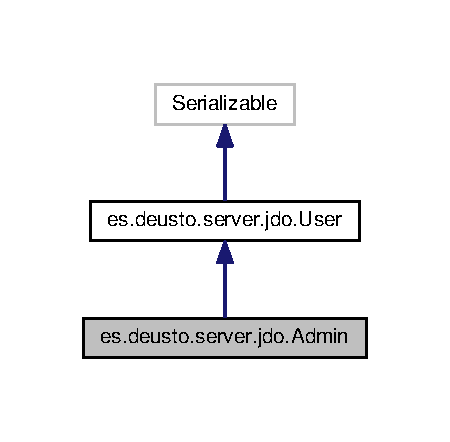
\includegraphics[width=216pt]{classes_1_1deusto_1_1server_1_1jdo_1_1_admin__inherit__graph}
\end{center}
\end{figure}


Collaboration diagram for es.\+deusto.\+server.\+jdo.\+Admin\+:
\nopagebreak
\begin{figure}[H]
\begin{center}
\leavevmode
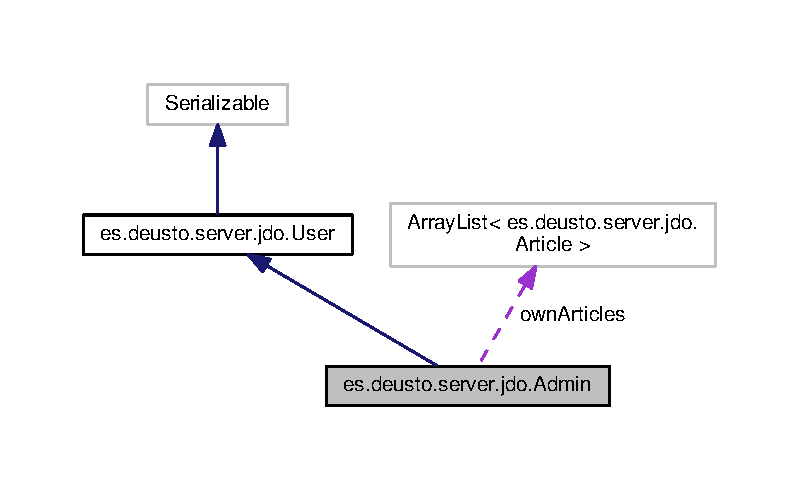
\includegraphics[width=350pt]{classes_1_1deusto_1_1server_1_1jdo_1_1_admin__coll__graph}
\end{center}
\end{figure}
\subsection*{Public Member Functions}
\begin{DoxyCompactItemize}
\item 
\hyperlink{classes_1_1deusto_1_1server_1_1jdo_1_1_admin_adf8cbc79ef2fe23545bde1a1dd635b08}{Admin} (String \hyperlink{classes_1_1deusto_1_1server_1_1jdo_1_1_user_aa1f05a7b487224d7c846fb81e5262c00}{username}, String \hyperlink{classes_1_1deusto_1_1server_1_1jdo_1_1_user_a9e3d470b8d2b36996759bd0595984870}{password}, String \hyperlink{classes_1_1deusto_1_1server_1_1jdo_1_1_user_a2aedb628a946e5044f27a3e6cbda31f0}{email}, Array\+List$<$ \hyperlink{classes_1_1deusto_1_1server_1_1jdo_1_1_article}{Article} $>$ articles)
\item 
\hyperlink{classes_1_1deusto_1_1server_1_1jdo_1_1_admin_ad1802d8f7e66466b71e3f8dd74a51af0}{Admin} (String \hyperlink{classes_1_1deusto_1_1server_1_1jdo_1_1_user_aa1f05a7b487224d7c846fb81e5262c00}{username}, String \hyperlink{classes_1_1deusto_1_1server_1_1jdo_1_1_user_a9e3d470b8d2b36996759bd0595984870}{password}, String \hyperlink{classes_1_1deusto_1_1server_1_1jdo_1_1_user_a2aedb628a946e5044f27a3e6cbda31f0}{email})
\item 
void \hyperlink{classes_1_1deusto_1_1server_1_1jdo_1_1_admin_a24c169163bc35735f4f02b9e4dc2514d}{add\+Article} (\hyperlink{classes_1_1deusto_1_1server_1_1jdo_1_1_article}{Article} article)
\item 
void \hyperlink{classes_1_1deusto_1_1server_1_1jdo_1_1_admin_a059fd0608e09ed77ed52bf31b54734e0}{delete\+Article} (\hyperlink{classes_1_1deusto_1_1server_1_1jdo_1_1_article}{Article} article)
\item 
Array\+List$<$ \hyperlink{classes_1_1deusto_1_1server_1_1jdo_1_1_article}{Article} $>$ \hyperlink{classes_1_1deusto_1_1server_1_1jdo_1_1_admin_a26e6fdf7339157c66b276bc20fdeca3c}{get\+Own\+Articles} ()
\item 
void \hyperlink{classes_1_1deusto_1_1server_1_1jdo_1_1_admin_abb330a6e4c9e543fff03ab213055c2c4}{set\+Own\+Articles} (Array\+List$<$ \hyperlink{classes_1_1deusto_1_1server_1_1jdo_1_1_article}{Article} $>$ \hyperlink{classes_1_1deusto_1_1server_1_1jdo_1_1_admin_aff35b2a52374104224e98ba92fd7eac3}{own\+Articles})
\end{DoxyCompactItemize}
\subsection*{Public Attributes}
\begin{DoxyCompactItemize}
\item 
Array\+List$<$ \hyperlink{classes_1_1deusto_1_1server_1_1jdo_1_1_article}{Article} $>$ \hyperlink{classes_1_1deusto_1_1server_1_1jdo_1_1_admin_aff35b2a52374104224e98ba92fd7eac3}{own\+Articles} = new Array\+List$<$\hyperlink{classes_1_1deusto_1_1server_1_1jdo_1_1_article}{Article}$>$()
\end{DoxyCompactItemize}
\subsection*{Additional Inherited Members}


\subsection{Detailed Description}
The class for the administrator. \begin{DoxyAuthor}{Author}
albertofdr 
\end{DoxyAuthor}


Definition at line 17 of file Admin.\+java.



\subsection{Constructor \& Destructor Documentation}
\mbox{\Hypertarget{classes_1_1deusto_1_1server_1_1jdo_1_1_admin_adf8cbc79ef2fe23545bde1a1dd635b08}\label{classes_1_1deusto_1_1server_1_1jdo_1_1_admin_adf8cbc79ef2fe23545bde1a1dd635b08}} 
\index{es\+::deusto\+::server\+::jdo\+::\+Admin@{es\+::deusto\+::server\+::jdo\+::\+Admin}!Admin@{Admin}}
\index{Admin@{Admin}!es\+::deusto\+::server\+::jdo\+::\+Admin@{es\+::deusto\+::server\+::jdo\+::\+Admin}}
\subsubsection{\texorpdfstring{Admin()}{Admin()}\hspace{0.1cm}{\footnotesize\ttfamily [1/2]}}
{\footnotesize\ttfamily es.\+deusto.\+server.\+jdo.\+Admin.\+Admin (\begin{DoxyParamCaption}\item[{String}]{username,  }\item[{String}]{password,  }\item[{String}]{email,  }\item[{Array\+List$<$ \hyperlink{classes_1_1deusto_1_1server_1_1jdo_1_1_article}{Article} $>$}]{articles }\end{DoxyParamCaption})}

Creates an \hyperlink{classes_1_1deusto_1_1server_1_1jdo_1_1_admin}{Admin} with her articles 
\begin{DoxyParams}{Parameters}
{\em username} & The username of the admin \\
\hline
{\em password} & The password of the admin \\
\hline
{\em email} & The email of the admin \\
\hline
{\em articles} & The articles of the admin \\
\hline
\end{DoxyParams}


Definition at line 30 of file Admin.\+java.

\mbox{\Hypertarget{classes_1_1deusto_1_1server_1_1jdo_1_1_admin_ad1802d8f7e66466b71e3f8dd74a51af0}\label{classes_1_1deusto_1_1server_1_1jdo_1_1_admin_ad1802d8f7e66466b71e3f8dd74a51af0}} 
\index{es\+::deusto\+::server\+::jdo\+::\+Admin@{es\+::deusto\+::server\+::jdo\+::\+Admin}!Admin@{Admin}}
\index{Admin@{Admin}!es\+::deusto\+::server\+::jdo\+::\+Admin@{es\+::deusto\+::server\+::jdo\+::\+Admin}}
\subsubsection{\texorpdfstring{Admin()}{Admin()}\hspace{0.1cm}{\footnotesize\ttfamily [2/2]}}
{\footnotesize\ttfamily es.\+deusto.\+server.\+jdo.\+Admin.\+Admin (\begin{DoxyParamCaption}\item[{String}]{username,  }\item[{String}]{password,  }\item[{String}]{email }\end{DoxyParamCaption})}

Creates an \hyperlink{classes_1_1deusto_1_1server_1_1jdo_1_1_admin}{Admin} with zero articles 
\begin{DoxyParams}{Parameters}
{\em username} & The username of the admin \\
\hline
{\em password} & The password of the admin \\
\hline
{\em email} & The email of the admin \\
\hline
\end{DoxyParams}


Definition at line 40 of file Admin.\+java.



\subsection{Member Function Documentation}
\mbox{\Hypertarget{classes_1_1deusto_1_1server_1_1jdo_1_1_admin_a24c169163bc35735f4f02b9e4dc2514d}\label{classes_1_1deusto_1_1server_1_1jdo_1_1_admin_a24c169163bc35735f4f02b9e4dc2514d}} 
\index{es\+::deusto\+::server\+::jdo\+::\+Admin@{es\+::deusto\+::server\+::jdo\+::\+Admin}!add\+Article@{add\+Article}}
\index{add\+Article@{add\+Article}!es\+::deusto\+::server\+::jdo\+::\+Admin@{es\+::deusto\+::server\+::jdo\+::\+Admin}}
\subsubsection{\texorpdfstring{add\+Article()}{addArticle()}}
{\footnotesize\ttfamily void es.\+deusto.\+server.\+jdo.\+Admin.\+add\+Article (\begin{DoxyParamCaption}\item[{\hyperlink{classes_1_1deusto_1_1server_1_1jdo_1_1_article}{Article}}]{article }\end{DoxyParamCaption})}


\begin{DoxyParams}{Parameters}
{\em article} & To add an article for the \hyperlink{classes_1_1deusto_1_1server_1_1jdo_1_1_admin}{Admin} \\
\hline
\end{DoxyParams}


Definition at line 52 of file Admin.\+java.

\mbox{\Hypertarget{classes_1_1deusto_1_1server_1_1jdo_1_1_admin_a059fd0608e09ed77ed52bf31b54734e0}\label{classes_1_1deusto_1_1server_1_1jdo_1_1_admin_a059fd0608e09ed77ed52bf31b54734e0}} 
\index{es\+::deusto\+::server\+::jdo\+::\+Admin@{es\+::deusto\+::server\+::jdo\+::\+Admin}!delete\+Article@{delete\+Article}}
\index{delete\+Article@{delete\+Article}!es\+::deusto\+::server\+::jdo\+::\+Admin@{es\+::deusto\+::server\+::jdo\+::\+Admin}}
\subsubsection{\texorpdfstring{delete\+Article()}{deleteArticle()}}
{\footnotesize\ttfamily void es.\+deusto.\+server.\+jdo.\+Admin.\+delete\+Article (\begin{DoxyParamCaption}\item[{\hyperlink{classes_1_1deusto_1_1server_1_1jdo_1_1_article}{Article}}]{article }\end{DoxyParamCaption})}


\begin{DoxyParams}{Parameters}
{\em article} & To delete an article \\
\hline
\end{DoxyParams}


Definition at line 62 of file Admin.\+java.

\mbox{\Hypertarget{classes_1_1deusto_1_1server_1_1jdo_1_1_admin_a26e6fdf7339157c66b276bc20fdeca3c}\label{classes_1_1deusto_1_1server_1_1jdo_1_1_admin_a26e6fdf7339157c66b276bc20fdeca3c}} 
\index{es\+::deusto\+::server\+::jdo\+::\+Admin@{es\+::deusto\+::server\+::jdo\+::\+Admin}!get\+Own\+Articles@{get\+Own\+Articles}}
\index{get\+Own\+Articles@{get\+Own\+Articles}!es\+::deusto\+::server\+::jdo\+::\+Admin@{es\+::deusto\+::server\+::jdo\+::\+Admin}}
\subsubsection{\texorpdfstring{get\+Own\+Articles()}{getOwnArticles()}}
{\footnotesize\ttfamily Array\+List$<$\hyperlink{classes_1_1deusto_1_1server_1_1jdo_1_1_article}{Article}$>$ es.\+deusto.\+server.\+jdo.\+Admin.\+get\+Own\+Articles (\begin{DoxyParamCaption}{ }\end{DoxyParamCaption})}

\begin{DoxyReturn}{Returns}
Returns the \hyperlink{classes_1_1deusto_1_1server_1_1jdo_1_1_admin}{Admin} articles 
\end{DoxyReturn}


Definition at line 72 of file Admin.\+java.

\mbox{\Hypertarget{classes_1_1deusto_1_1server_1_1jdo_1_1_admin_abb330a6e4c9e543fff03ab213055c2c4}\label{classes_1_1deusto_1_1server_1_1jdo_1_1_admin_abb330a6e4c9e543fff03ab213055c2c4}} 
\index{es\+::deusto\+::server\+::jdo\+::\+Admin@{es\+::deusto\+::server\+::jdo\+::\+Admin}!set\+Own\+Articles@{set\+Own\+Articles}}
\index{set\+Own\+Articles@{set\+Own\+Articles}!es\+::deusto\+::server\+::jdo\+::\+Admin@{es\+::deusto\+::server\+::jdo\+::\+Admin}}
\subsubsection{\texorpdfstring{set\+Own\+Articles()}{setOwnArticles()}}
{\footnotesize\ttfamily void es.\+deusto.\+server.\+jdo.\+Admin.\+set\+Own\+Articles (\begin{DoxyParamCaption}\item[{Array\+List$<$ \hyperlink{classes_1_1deusto_1_1server_1_1jdo_1_1_article}{Article} $>$}]{own\+Articles }\end{DoxyParamCaption})}


\begin{DoxyParams}{Parameters}
{\em own\+Articles} & To set articles \\
\hline
\end{DoxyParams}


Definition at line 80 of file Admin.\+java.



\subsection{Member Data Documentation}
\mbox{\Hypertarget{classes_1_1deusto_1_1server_1_1jdo_1_1_admin_aff35b2a52374104224e98ba92fd7eac3}\label{classes_1_1deusto_1_1server_1_1jdo_1_1_admin_aff35b2a52374104224e98ba92fd7eac3}} 
\index{es\+::deusto\+::server\+::jdo\+::\+Admin@{es\+::deusto\+::server\+::jdo\+::\+Admin}!own\+Articles@{own\+Articles}}
\index{own\+Articles@{own\+Articles}!es\+::deusto\+::server\+::jdo\+::\+Admin@{es\+::deusto\+::server\+::jdo\+::\+Admin}}
\subsubsection{\texorpdfstring{own\+Articles}{ownArticles}}
{\footnotesize\ttfamily Array\+List$<$\hyperlink{classes_1_1deusto_1_1server_1_1jdo_1_1_article}{Article}$>$ es.\+deusto.\+server.\+jdo.\+Admin.\+own\+Articles = new Array\+List$<$\hyperlink{classes_1_1deusto_1_1server_1_1jdo_1_1_article}{Article}$>$()}



Definition at line 21 of file Admin.\+java.



The documentation for this class was generated from the following file\+:\begin{DoxyCompactItemize}
\item 
src/main/java/es/deusto/server/jdo/\hyperlink{_admin_8java}{Admin.\+java}\end{DoxyCompactItemize}

\hypertarget{classes_1_1deusto_1_1server_1_1jdo_1_1_admin_test}{}\section{es.\+deusto.\+server.\+jdo.\+Admin\+Test Class Reference}
\label{classes_1_1deusto_1_1server_1_1jdo_1_1_admin_test}\index{es.\+deusto.\+server.\+jdo.\+Admin\+Test@{es.\+deusto.\+server.\+jdo.\+Admin\+Test}}


Collaboration diagram for es.\+deusto.\+server.\+jdo.\+Admin\+Test\+:\nopagebreak
\begin{figure}[H]
\begin{center}
\leavevmode
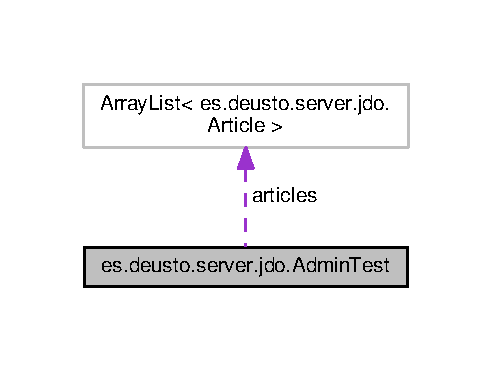
\includegraphics[width=236pt]{classes_1_1deusto_1_1server_1_1jdo_1_1_admin_test__coll__graph}
\end{center}
\end{figure}
\subsection*{Public Member Functions}
\begin{DoxyCompactItemize}
\item 
void \hyperlink{classes_1_1deusto_1_1server_1_1jdo_1_1_admin_test_acaa555000602cd83a7e73550a7f114b4}{set\+Up} ()
\item 
.junit.\+Test void \hyperlink{classes_1_1deusto_1_1server_1_1jdo_1_1_admin_test_aba3d4e2c7110a3bc1c7557f4491e1691}{test\+App} ()
\end{DoxyCompactItemize}
\subsection*{Static Public Member Functions}
\begin{DoxyCompactItemize}
\item 
static junit.\+framework.\+Test \hyperlink{classes_1_1deusto_1_1server_1_1jdo_1_1_admin_test_aa2992f98029130ba303b2a7753d3c35d}{suite} ()
\end{DoxyCompactItemize}


\subsection{Detailed Description}


Definition at line 17 of file Admin\+Test.\+java.



\subsection{Member Function Documentation}
\mbox{\Hypertarget{classes_1_1deusto_1_1server_1_1jdo_1_1_admin_test_acaa555000602cd83a7e73550a7f114b4}\label{classes_1_1deusto_1_1server_1_1jdo_1_1_admin_test_acaa555000602cd83a7e73550a7f114b4}} 
\index{es\+::deusto\+::server\+::jdo\+::\+Admin\+Test@{es\+::deusto\+::server\+::jdo\+::\+Admin\+Test}!set\+Up@{set\+Up}}
\index{set\+Up@{set\+Up}!es\+::deusto\+::server\+::jdo\+::\+Admin\+Test@{es\+::deusto\+::server\+::jdo\+::\+Admin\+Test}}
\subsubsection{\texorpdfstring{set\+Up()}{setUp()}}
{\footnotesize\ttfamily void es.\+deusto.\+server.\+jdo.\+Admin\+Test.\+set\+Up (\begin{DoxyParamCaption}{ }\end{DoxyParamCaption})}

Create the test case


\begin{DoxyParams}{Parameters}
{\em test\+Name} & name of the test case \\
\hline
\end{DoxyParams}
\begin{DoxyReturn}{Returns}

\end{DoxyReturn}


Definition at line 41 of file Admin\+Test.\+java.

\mbox{\Hypertarget{classes_1_1deusto_1_1server_1_1jdo_1_1_admin_test_aa2992f98029130ba303b2a7753d3c35d}\label{classes_1_1deusto_1_1server_1_1jdo_1_1_admin_test_aa2992f98029130ba303b2a7753d3c35d}} 
\index{es\+::deusto\+::server\+::jdo\+::\+Admin\+Test@{es\+::deusto\+::server\+::jdo\+::\+Admin\+Test}!suite@{suite}}
\index{suite@{suite}!es\+::deusto\+::server\+::jdo\+::\+Admin\+Test@{es\+::deusto\+::server\+::jdo\+::\+Admin\+Test}}
\subsubsection{\texorpdfstring{suite()}{suite()}}
{\footnotesize\ttfamily static junit.\+framework.\+Test es.\+deusto.\+server.\+jdo.\+Admin\+Test.\+suite (\begin{DoxyParamCaption}{ }\end{DoxyParamCaption})\hspace{0.3cm}{\ttfamily [static]}}

\begin{DoxyReturn}{Returns}
the suite of tests being tested 
\end{DoxyReturn}


Definition at line 30 of file Admin\+Test.\+java.

\mbox{\Hypertarget{classes_1_1deusto_1_1server_1_1jdo_1_1_admin_test_aba3d4e2c7110a3bc1c7557f4491e1691}\label{classes_1_1deusto_1_1server_1_1jdo_1_1_admin_test_aba3d4e2c7110a3bc1c7557f4491e1691}} 
\index{es\+::deusto\+::server\+::jdo\+::\+Admin\+Test@{es\+::deusto\+::server\+::jdo\+::\+Admin\+Test}!test\+App@{test\+App}}
\index{test\+App@{test\+App}!es\+::deusto\+::server\+::jdo\+::\+Admin\+Test@{es\+::deusto\+::server\+::jdo\+::\+Admin\+Test}}
\subsubsection{\texorpdfstring{test\+App()}{testApp()}}
{\footnotesize\ttfamily .junit.\+Test void es.\+deusto.\+server.\+jdo.\+Admin\+Test.\+test\+App (\begin{DoxyParamCaption}{ }\end{DoxyParamCaption})}

Test of the data 

Definition at line 61 of file Admin\+Test.\+java.



The documentation for this class was generated from the following file\+:\begin{DoxyCompactItemize}
\item 
/home/albertofdr/git/\+B\+S\+P\+Q19-\/\+E3/src/test/java/es/deusto/server/jdo/\hyperlink{_admin_test_8java}{Admin\+Test.\+java}\end{DoxyCompactItemize}

\hypertarget{classes_1_1deusto_1_1server_1_1jdo_1_1_article}{}\section{es.\+deusto.\+server.\+jdo.\+Article Class Reference}
\label{classes_1_1deusto_1_1server_1_1jdo_1_1_article}\index{es.\+deusto.\+server.\+jdo.\+Article@{es.\+deusto.\+server.\+jdo.\+Article}}


Inheritance diagram for es.\+deusto.\+server.\+jdo.\+Article\+:\nopagebreak
\begin{figure}[H]
\begin{center}
\leavevmode
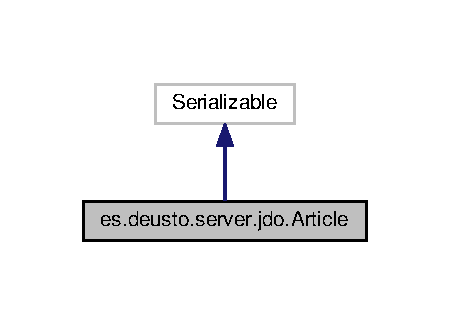
\includegraphics[width=216pt]{classes_1_1deusto_1_1server_1_1jdo_1_1_article__inherit__graph}
\end{center}
\end{figure}


Collaboration diagram for es.\+deusto.\+server.\+jdo.\+Article\+:\nopagebreak
\begin{figure}[H]
\begin{center}
\leavevmode
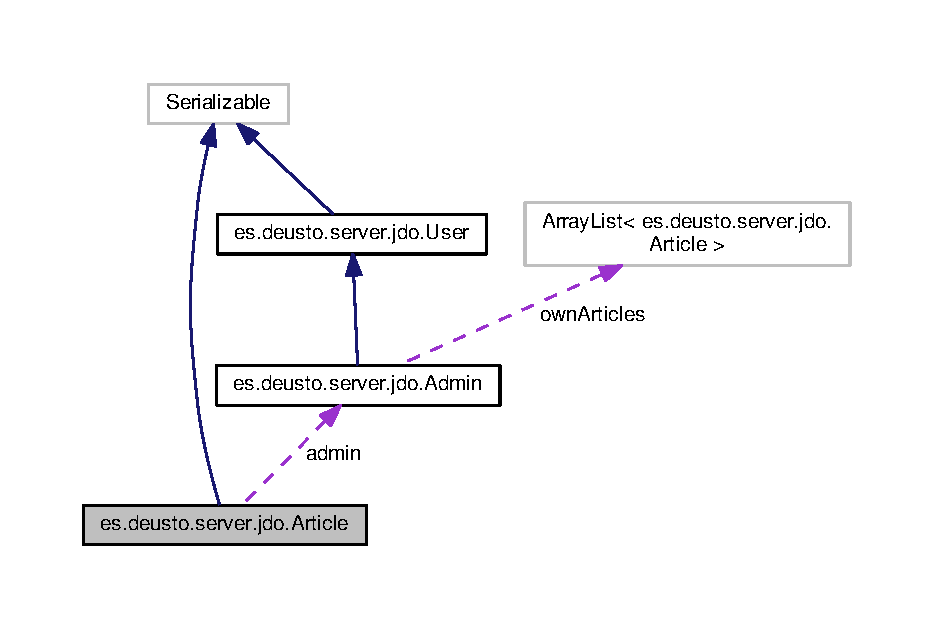
\includegraphics[width=350pt]{classes_1_1deusto_1_1server_1_1jdo_1_1_article__coll__graph}
\end{center}
\end{figure}
\subsection*{Public Member Functions}
\begin{DoxyCompactItemize}
\item 
\hyperlink{classes_1_1deusto_1_1server_1_1jdo_1_1_article_a74089feda9d822eb36d981dccb7bc4c7}{Article} (String \hyperlink{classes_1_1deusto_1_1server_1_1jdo_1_1_article_a94695d557769f2abe9dee76224e4376b}{title}, String \hyperlink{classes_1_1deusto_1_1server_1_1jdo_1_1_article_a1dd07a7780e5b7f0bedd0fbabf85d587}{body}, String \hyperlink{classes_1_1deusto_1_1server_1_1jdo_1_1_article_a4ece506f3c446ae045c821f68fd335ce}{category}, int \hyperlink{classes_1_1deusto_1_1server_1_1jdo_1_1_article_aa2d904e39c1518acd505ebd21b9bd156}{visits}, \hyperlink{classes_1_1deusto_1_1server_1_1jdo_1_1_admin}{Admin} \hyperlink{classes_1_1deusto_1_1server_1_1jdo_1_1_article_a3c67e3be7d33d08209a92817a69d9020}{admin})
\item 
\hyperlink{classes_1_1deusto_1_1server_1_1jdo_1_1_article_a083d627c016ba19fad5f4a719da72cd4}{Article} (String \hyperlink{classes_1_1deusto_1_1server_1_1jdo_1_1_article_a94695d557769f2abe9dee76224e4376b}{title}, String \hyperlink{classes_1_1deusto_1_1server_1_1jdo_1_1_article_a1dd07a7780e5b7f0bedd0fbabf85d587}{body}, String \hyperlink{classes_1_1deusto_1_1server_1_1jdo_1_1_article_a4ece506f3c446ae045c821f68fd335ce}{category}, \hyperlink{classes_1_1deusto_1_1server_1_1jdo_1_1_admin}{Admin} \hyperlink{classes_1_1deusto_1_1server_1_1jdo_1_1_article_a3c67e3be7d33d08209a92817a69d9020}{admin})
\item 
String \hyperlink{classes_1_1deusto_1_1server_1_1jdo_1_1_article_a2b35e53280b447706cfe2ee8c8eabaac}{get\+Title} ()
\item 
void \hyperlink{classes_1_1deusto_1_1server_1_1jdo_1_1_article_a9ce648f3e251a70a23f095049cd42e63}{set\+Title} (String \hyperlink{classes_1_1deusto_1_1server_1_1jdo_1_1_article_a94695d557769f2abe9dee76224e4376b}{title})
\item 
String \hyperlink{classes_1_1deusto_1_1server_1_1jdo_1_1_article_a8fa1d3a79b76f42058e922c4e32fb197}{get\+Body} ()
\item 
void \hyperlink{classes_1_1deusto_1_1server_1_1jdo_1_1_article_a5160202c2a15e13a3acb376be95af99c}{set\+Body} (String \hyperlink{classes_1_1deusto_1_1server_1_1jdo_1_1_article_a1dd07a7780e5b7f0bedd0fbabf85d587}{body})
\item 
int \hyperlink{classes_1_1deusto_1_1server_1_1jdo_1_1_article_a0d14a1b74ec663f4e25780f9d1b2cf4f}{get\+Visits} ()
\item 
void \hyperlink{classes_1_1deusto_1_1server_1_1jdo_1_1_article_a0804eae1dafaa95ab89d2f481535ebf2}{set\+Visits} (int \hyperlink{classes_1_1deusto_1_1server_1_1jdo_1_1_article_aa2d904e39c1518acd505ebd21b9bd156}{visits})
\item 
String \hyperlink{classes_1_1deusto_1_1server_1_1jdo_1_1_article_a23780eedb093f3edd43a63c17e7684e4}{get\+Category} ()
\item 
void \hyperlink{classes_1_1deusto_1_1server_1_1jdo_1_1_article_aff563311f5d736b7e3e9394072957c2c}{set\+Category} (String \hyperlink{classes_1_1deusto_1_1server_1_1jdo_1_1_article_a4ece506f3c446ae045c821f68fd335ce}{category})
\item 
boolean \hyperlink{classes_1_1deusto_1_1server_1_1jdo_1_1_article_aa141b087b5291e238f218d275ba5dfbe}{equals} (\hyperlink{classes_1_1deusto_1_1server_1_1jdo_1_1_article}{Article} obj)
\item 
int \hyperlink{classes_1_1deusto_1_1server_1_1jdo_1_1_article_a19bd65f3359a77e3a41fb6973a583428}{hash\+Code} ()
\item 
String \hyperlink{classes_1_1deusto_1_1server_1_1jdo_1_1_article_a662ad7c662e2077076399e756e0731bf}{to\+String} ()
\item 
\hyperlink{classes_1_1deusto_1_1server_1_1jdo_1_1_admin}{Admin} \hyperlink{classes_1_1deusto_1_1server_1_1jdo_1_1_article_a61bf2e2f04b3bf40e2e85321efca5944}{get\+Admin} ()
\item 
void \hyperlink{classes_1_1deusto_1_1server_1_1jdo_1_1_article_ad8b51e19c966a54e8b4eb01fa4087671}{set\+Admin} (\hyperlink{classes_1_1deusto_1_1server_1_1jdo_1_1_admin}{Admin} \hyperlink{classes_1_1deusto_1_1server_1_1jdo_1_1_article_a3c67e3be7d33d08209a92817a69d9020}{admin})
\end{DoxyCompactItemize}
\subsection*{Public Attributes}
\begin{DoxyCompactItemize}
\item 
String \hyperlink{classes_1_1deusto_1_1server_1_1jdo_1_1_article_a94695d557769f2abe9dee76224e4376b}{title} = \char`\"{}\char`\"{}
\item 
String \hyperlink{classes_1_1deusto_1_1server_1_1jdo_1_1_article_a1dd07a7780e5b7f0bedd0fbabf85d587}{body} = \char`\"{}\char`\"{}
\item 
int \hyperlink{classes_1_1deusto_1_1server_1_1jdo_1_1_article_aa2d904e39c1518acd505ebd21b9bd156}{visits} = 0
\item 
String \hyperlink{classes_1_1deusto_1_1server_1_1jdo_1_1_article_a4ece506f3c446ae045c821f68fd335ce}{category} = \char`\"{}\char`\"{}
\item 
\hyperlink{classes_1_1deusto_1_1server_1_1jdo_1_1_admin}{Admin} \hyperlink{classes_1_1deusto_1_1server_1_1jdo_1_1_article_a3c67e3be7d33d08209a92817a69d9020}{admin} = null
\end{DoxyCompactItemize}


\subsection{Detailed Description}
The class for the \hyperlink{classes_1_1deusto_1_1server_1_1jdo_1_1_article}{Article}. \begin{DoxyAuthor}{Author}
albertofdr 
\end{DoxyAuthor}


Definition at line 15 of file Article.\+java.



\subsection{Constructor \& Destructor Documentation}
\mbox{\Hypertarget{classes_1_1deusto_1_1server_1_1jdo_1_1_article_a74089feda9d822eb36d981dccb7bc4c7}\label{classes_1_1deusto_1_1server_1_1jdo_1_1_article_a74089feda9d822eb36d981dccb7bc4c7}} 
\index{es\+::deusto\+::server\+::jdo\+::\+Article@{es\+::deusto\+::server\+::jdo\+::\+Article}!Article@{Article}}
\index{Article@{Article}!es\+::deusto\+::server\+::jdo\+::\+Article@{es\+::deusto\+::server\+::jdo\+::\+Article}}
\subsubsection{\texorpdfstring{Article()}{Article()}\hspace{0.1cm}{\footnotesize\ttfamily [1/2]}}
{\footnotesize\ttfamily es.\+deusto.\+server.\+jdo.\+Article.\+Article (\begin{DoxyParamCaption}\item[{String}]{title,  }\item[{String}]{body,  }\item[{String}]{category,  }\item[{int}]{visits,  }\item[{\hyperlink{classes_1_1deusto_1_1server_1_1jdo_1_1_admin}{Admin}}]{admin }\end{DoxyParamCaption})}

Constructor where you can also set the visits 
\begin{DoxyParams}{Parameters}
{\em title} & The title for the article \\
\hline
{\em body} & The body of the article \\
\hline
{\em visits} & How many visits the article have \\
\hline
{\em category} & The category of the article \\
\hline
\end{DoxyParams}


Definition at line 30 of file Article.\+java.

\mbox{\Hypertarget{classes_1_1deusto_1_1server_1_1jdo_1_1_article_a083d627c016ba19fad5f4a719da72cd4}\label{classes_1_1deusto_1_1server_1_1jdo_1_1_article_a083d627c016ba19fad5f4a719da72cd4}} 
\index{es\+::deusto\+::server\+::jdo\+::\+Article@{es\+::deusto\+::server\+::jdo\+::\+Article}!Article@{Article}}
\index{Article@{Article}!es\+::deusto\+::server\+::jdo\+::\+Article@{es\+::deusto\+::server\+::jdo\+::\+Article}}
\subsubsection{\texorpdfstring{Article()}{Article()}\hspace{0.1cm}{\footnotesize\ttfamily [2/2]}}
{\footnotesize\ttfamily es.\+deusto.\+server.\+jdo.\+Article.\+Article (\begin{DoxyParamCaption}\item[{String}]{title,  }\item[{String}]{body,  }\item[{String}]{category,  }\item[{\hyperlink{classes_1_1deusto_1_1server_1_1jdo_1_1_admin}{Admin}}]{admin }\end{DoxyParamCaption})}

Constructor for a new article where you can\textquotesingle{}t set the visits (Visits == 0) 
\begin{DoxyParams}{Parameters}
{\em title} & The title for the article \\
\hline
{\em body} & The body of the article \\
\hline
{\em category} & The category of the article \\
\hline
\end{DoxyParams}


Definition at line 45 of file Article.\+java.



\subsection{Member Function Documentation}
\mbox{\Hypertarget{classes_1_1deusto_1_1server_1_1jdo_1_1_article_aa141b087b5291e238f218d275ba5dfbe}\label{classes_1_1deusto_1_1server_1_1jdo_1_1_article_aa141b087b5291e238f218d275ba5dfbe}} 
\index{es\+::deusto\+::server\+::jdo\+::\+Article@{es\+::deusto\+::server\+::jdo\+::\+Article}!equals@{equals}}
\index{equals@{equals}!es\+::deusto\+::server\+::jdo\+::\+Article@{es\+::deusto\+::server\+::jdo\+::\+Article}}
\subsubsection{\texorpdfstring{equals()}{equals()}}
{\footnotesize\ttfamily boolean es.\+deusto.\+server.\+jdo.\+Article.\+equals (\begin{DoxyParamCaption}\item[{\hyperlink{classes_1_1deusto_1_1server_1_1jdo_1_1_article}{Article}}]{obj }\end{DoxyParamCaption})}

Compare two articles 
\begin{DoxyParams}{Parameters}
{\em obj} & The article to compare with \\
\hline
\end{DoxyParams}
\begin{DoxyReturn}{Returns}
If they are equal or not 
\end{DoxyReturn}


Definition at line 126 of file Article.\+java.

\mbox{\Hypertarget{classes_1_1deusto_1_1server_1_1jdo_1_1_article_a61bf2e2f04b3bf40e2e85321efca5944}\label{classes_1_1deusto_1_1server_1_1jdo_1_1_article_a61bf2e2f04b3bf40e2e85321efca5944}} 
\index{es\+::deusto\+::server\+::jdo\+::\+Article@{es\+::deusto\+::server\+::jdo\+::\+Article}!get\+Admin@{get\+Admin}}
\index{get\+Admin@{get\+Admin}!es\+::deusto\+::server\+::jdo\+::\+Article@{es\+::deusto\+::server\+::jdo\+::\+Article}}
\subsubsection{\texorpdfstring{get\+Admin()}{getAdmin()}}
{\footnotesize\ttfamily \hyperlink{classes_1_1deusto_1_1server_1_1jdo_1_1_admin}{Admin} es.\+deusto.\+server.\+jdo.\+Article.\+get\+Admin (\begin{DoxyParamCaption}{ }\end{DoxyParamCaption})}



Definition at line 147 of file Article.\+java.

\mbox{\Hypertarget{classes_1_1deusto_1_1server_1_1jdo_1_1_article_a8fa1d3a79b76f42058e922c4e32fb197}\label{classes_1_1deusto_1_1server_1_1jdo_1_1_article_a8fa1d3a79b76f42058e922c4e32fb197}} 
\index{es\+::deusto\+::server\+::jdo\+::\+Article@{es\+::deusto\+::server\+::jdo\+::\+Article}!get\+Body@{get\+Body}}
\index{get\+Body@{get\+Body}!es\+::deusto\+::server\+::jdo\+::\+Article@{es\+::deusto\+::server\+::jdo\+::\+Article}}
\subsubsection{\texorpdfstring{get\+Body()}{getBody()}}
{\footnotesize\ttfamily String es.\+deusto.\+server.\+jdo.\+Article.\+get\+Body (\begin{DoxyParamCaption}{ }\end{DoxyParamCaption})}

\begin{DoxyReturn}{Returns}
Return the body of the article 
\end{DoxyReturn}


Definition at line 77 of file Article.\+java.

\mbox{\Hypertarget{classes_1_1deusto_1_1server_1_1jdo_1_1_article_a23780eedb093f3edd43a63c17e7684e4}\label{classes_1_1deusto_1_1server_1_1jdo_1_1_article_a23780eedb093f3edd43a63c17e7684e4}} 
\index{es\+::deusto\+::server\+::jdo\+::\+Article@{es\+::deusto\+::server\+::jdo\+::\+Article}!get\+Category@{get\+Category}}
\index{get\+Category@{get\+Category}!es\+::deusto\+::server\+::jdo\+::\+Article@{es\+::deusto\+::server\+::jdo\+::\+Article}}
\subsubsection{\texorpdfstring{get\+Category()}{getCategory()}}
{\footnotesize\ttfamily String es.\+deusto.\+server.\+jdo.\+Article.\+get\+Category (\begin{DoxyParamCaption}{ }\end{DoxyParamCaption})}

\begin{DoxyReturn}{Returns}
Gets you the category of the article 
\end{DoxyReturn}


Definition at line 109 of file Article.\+java.

\mbox{\Hypertarget{classes_1_1deusto_1_1server_1_1jdo_1_1_article_a2b35e53280b447706cfe2ee8c8eabaac}\label{classes_1_1deusto_1_1server_1_1jdo_1_1_article_a2b35e53280b447706cfe2ee8c8eabaac}} 
\index{es\+::deusto\+::server\+::jdo\+::\+Article@{es\+::deusto\+::server\+::jdo\+::\+Article}!get\+Title@{get\+Title}}
\index{get\+Title@{get\+Title}!es\+::deusto\+::server\+::jdo\+::\+Article@{es\+::deusto\+::server\+::jdo\+::\+Article}}
\subsubsection{\texorpdfstring{get\+Title()}{getTitle()}}
{\footnotesize\ttfamily String es.\+deusto.\+server.\+jdo.\+Article.\+get\+Title (\begin{DoxyParamCaption}{ }\end{DoxyParamCaption})}

\begin{DoxyReturn}{Returns}
The title of this article 
\end{DoxyReturn}


Definition at line 61 of file Article.\+java.

\mbox{\Hypertarget{classes_1_1deusto_1_1server_1_1jdo_1_1_article_a0d14a1b74ec663f4e25780f9d1b2cf4f}\label{classes_1_1deusto_1_1server_1_1jdo_1_1_article_a0d14a1b74ec663f4e25780f9d1b2cf4f}} 
\index{es\+::deusto\+::server\+::jdo\+::\+Article@{es\+::deusto\+::server\+::jdo\+::\+Article}!get\+Visits@{get\+Visits}}
\index{get\+Visits@{get\+Visits}!es\+::deusto\+::server\+::jdo\+::\+Article@{es\+::deusto\+::server\+::jdo\+::\+Article}}
\subsubsection{\texorpdfstring{get\+Visits()}{getVisits()}}
{\footnotesize\ttfamily int es.\+deusto.\+server.\+jdo.\+Article.\+get\+Visits (\begin{DoxyParamCaption}{ }\end{DoxyParamCaption})}

\begin{DoxyReturn}{Returns}
Return the visits of the article 
\end{DoxyReturn}


Definition at line 93 of file Article.\+java.

\mbox{\Hypertarget{classes_1_1deusto_1_1server_1_1jdo_1_1_article_a19bd65f3359a77e3a41fb6973a583428}\label{classes_1_1deusto_1_1server_1_1jdo_1_1_article_a19bd65f3359a77e3a41fb6973a583428}} 
\index{es\+::deusto\+::server\+::jdo\+::\+Article@{es\+::deusto\+::server\+::jdo\+::\+Article}!hash\+Code@{hash\+Code}}
\index{hash\+Code@{hash\+Code}!es\+::deusto\+::server\+::jdo\+::\+Article@{es\+::deusto\+::server\+::jdo\+::\+Article}}
\subsubsection{\texorpdfstring{hash\+Code()}{hashCode()}}
{\footnotesize\ttfamily int es.\+deusto.\+server.\+jdo.\+Article.\+hash\+Code (\begin{DoxyParamCaption}{ }\end{DoxyParamCaption})}

Hashcode for the article 

Definition at line 136 of file Article.\+java.

\mbox{\Hypertarget{classes_1_1deusto_1_1server_1_1jdo_1_1_article_ad8b51e19c966a54e8b4eb01fa4087671}\label{classes_1_1deusto_1_1server_1_1jdo_1_1_article_ad8b51e19c966a54e8b4eb01fa4087671}} 
\index{es\+::deusto\+::server\+::jdo\+::\+Article@{es\+::deusto\+::server\+::jdo\+::\+Article}!set\+Admin@{set\+Admin}}
\index{set\+Admin@{set\+Admin}!es\+::deusto\+::server\+::jdo\+::\+Article@{es\+::deusto\+::server\+::jdo\+::\+Article}}
\subsubsection{\texorpdfstring{set\+Admin()}{setAdmin()}}
{\footnotesize\ttfamily void es.\+deusto.\+server.\+jdo.\+Article.\+set\+Admin (\begin{DoxyParamCaption}\item[{\hyperlink{classes_1_1deusto_1_1server_1_1jdo_1_1_admin}{Admin}}]{admin }\end{DoxyParamCaption})}



Definition at line 151 of file Article.\+java.

\mbox{\Hypertarget{classes_1_1deusto_1_1server_1_1jdo_1_1_article_a5160202c2a15e13a3acb376be95af99c}\label{classes_1_1deusto_1_1server_1_1jdo_1_1_article_a5160202c2a15e13a3acb376be95af99c}} 
\index{es\+::deusto\+::server\+::jdo\+::\+Article@{es\+::deusto\+::server\+::jdo\+::\+Article}!set\+Body@{set\+Body}}
\index{set\+Body@{set\+Body}!es\+::deusto\+::server\+::jdo\+::\+Article@{es\+::deusto\+::server\+::jdo\+::\+Article}}
\subsubsection{\texorpdfstring{set\+Body()}{setBody()}}
{\footnotesize\ttfamily void es.\+deusto.\+server.\+jdo.\+Article.\+set\+Body (\begin{DoxyParamCaption}\item[{String}]{body }\end{DoxyParamCaption})}


\begin{DoxyParams}{Parameters}
{\em body} & Set the new body of the article \\
\hline
\end{DoxyParams}


Definition at line 85 of file Article.\+java.

\mbox{\Hypertarget{classes_1_1deusto_1_1server_1_1jdo_1_1_article_aff563311f5d736b7e3e9394072957c2c}\label{classes_1_1deusto_1_1server_1_1jdo_1_1_article_aff563311f5d736b7e3e9394072957c2c}} 
\index{es\+::deusto\+::server\+::jdo\+::\+Article@{es\+::deusto\+::server\+::jdo\+::\+Article}!set\+Category@{set\+Category}}
\index{set\+Category@{set\+Category}!es\+::deusto\+::server\+::jdo\+::\+Article@{es\+::deusto\+::server\+::jdo\+::\+Article}}
\subsubsection{\texorpdfstring{set\+Category()}{setCategory()}}
{\footnotesize\ttfamily void es.\+deusto.\+server.\+jdo.\+Article.\+set\+Category (\begin{DoxyParamCaption}\item[{String}]{category }\end{DoxyParamCaption})}


\begin{DoxyParams}{Parameters}
{\em category} & To set a new category of the article \\
\hline
\end{DoxyParams}


Definition at line 117 of file Article.\+java.

\mbox{\Hypertarget{classes_1_1deusto_1_1server_1_1jdo_1_1_article_a9ce648f3e251a70a23f095049cd42e63}\label{classes_1_1deusto_1_1server_1_1jdo_1_1_article_a9ce648f3e251a70a23f095049cd42e63}} 
\index{es\+::deusto\+::server\+::jdo\+::\+Article@{es\+::deusto\+::server\+::jdo\+::\+Article}!set\+Title@{set\+Title}}
\index{set\+Title@{set\+Title}!es\+::deusto\+::server\+::jdo\+::\+Article@{es\+::deusto\+::server\+::jdo\+::\+Article}}
\subsubsection{\texorpdfstring{set\+Title()}{setTitle()}}
{\footnotesize\ttfamily void es.\+deusto.\+server.\+jdo.\+Article.\+set\+Title (\begin{DoxyParamCaption}\item[{String}]{title }\end{DoxyParamCaption})}


\begin{DoxyParams}{Parameters}
{\em title} & To set a new title \\
\hline
\end{DoxyParams}


Definition at line 69 of file Article.\+java.

\mbox{\Hypertarget{classes_1_1deusto_1_1server_1_1jdo_1_1_article_a0804eae1dafaa95ab89d2f481535ebf2}\label{classes_1_1deusto_1_1server_1_1jdo_1_1_article_a0804eae1dafaa95ab89d2f481535ebf2}} 
\index{es\+::deusto\+::server\+::jdo\+::\+Article@{es\+::deusto\+::server\+::jdo\+::\+Article}!set\+Visits@{set\+Visits}}
\index{set\+Visits@{set\+Visits}!es\+::deusto\+::server\+::jdo\+::\+Article@{es\+::deusto\+::server\+::jdo\+::\+Article}}
\subsubsection{\texorpdfstring{set\+Visits()}{setVisits()}}
{\footnotesize\ttfamily void es.\+deusto.\+server.\+jdo.\+Article.\+set\+Visits (\begin{DoxyParamCaption}\item[{int}]{visits }\end{DoxyParamCaption})}


\begin{DoxyParams}{Parameters}
{\em visits} & To set how many visits the article has \\
\hline
\end{DoxyParams}


Definition at line 101 of file Article.\+java.

\mbox{\Hypertarget{classes_1_1deusto_1_1server_1_1jdo_1_1_article_a662ad7c662e2077076399e756e0731bf}\label{classes_1_1deusto_1_1server_1_1jdo_1_1_article_a662ad7c662e2077076399e756e0731bf}} 
\index{es\+::deusto\+::server\+::jdo\+::\+Article@{es\+::deusto\+::server\+::jdo\+::\+Article}!to\+String@{to\+String}}
\index{to\+String@{to\+String}!es\+::deusto\+::server\+::jdo\+::\+Article@{es\+::deusto\+::server\+::jdo\+::\+Article}}
\subsubsection{\texorpdfstring{to\+String()}{toString()}}
{\footnotesize\ttfamily String es.\+deusto.\+server.\+jdo.\+Article.\+to\+String (\begin{DoxyParamCaption}{ }\end{DoxyParamCaption})}

Method to print the article 

Definition at line 143 of file Article.\+java.



\subsection{Member Data Documentation}
\mbox{\Hypertarget{classes_1_1deusto_1_1server_1_1jdo_1_1_article_a3c67e3be7d33d08209a92817a69d9020}\label{classes_1_1deusto_1_1server_1_1jdo_1_1_article_a3c67e3be7d33d08209a92817a69d9020}} 
\index{es\+::deusto\+::server\+::jdo\+::\+Article@{es\+::deusto\+::server\+::jdo\+::\+Article}!admin@{admin}}
\index{admin@{admin}!es\+::deusto\+::server\+::jdo\+::\+Article@{es\+::deusto\+::server\+::jdo\+::\+Article}}
\subsubsection{\texorpdfstring{admin}{admin}}
{\footnotesize\ttfamily \hyperlink{classes_1_1deusto_1_1server_1_1jdo_1_1_admin}{Admin} es.\+deusto.\+server.\+jdo.\+Article.\+admin = null}



Definition at line 22 of file Article.\+java.

\mbox{\Hypertarget{classes_1_1deusto_1_1server_1_1jdo_1_1_article_a1dd07a7780e5b7f0bedd0fbabf85d587}\label{classes_1_1deusto_1_1server_1_1jdo_1_1_article_a1dd07a7780e5b7f0bedd0fbabf85d587}} 
\index{es\+::deusto\+::server\+::jdo\+::\+Article@{es\+::deusto\+::server\+::jdo\+::\+Article}!body@{body}}
\index{body@{body}!es\+::deusto\+::server\+::jdo\+::\+Article@{es\+::deusto\+::server\+::jdo\+::\+Article}}
\subsubsection{\texorpdfstring{body}{body}}
{\footnotesize\ttfamily String es.\+deusto.\+server.\+jdo.\+Article.\+body = \char`\"{}\char`\"{}}



Definition at line 19 of file Article.\+java.

\mbox{\Hypertarget{classes_1_1deusto_1_1server_1_1jdo_1_1_article_a4ece506f3c446ae045c821f68fd335ce}\label{classes_1_1deusto_1_1server_1_1jdo_1_1_article_a4ece506f3c446ae045c821f68fd335ce}} 
\index{es\+::deusto\+::server\+::jdo\+::\+Article@{es\+::deusto\+::server\+::jdo\+::\+Article}!category@{category}}
\index{category@{category}!es\+::deusto\+::server\+::jdo\+::\+Article@{es\+::deusto\+::server\+::jdo\+::\+Article}}
\subsubsection{\texorpdfstring{category}{category}}
{\footnotesize\ttfamily String es.\+deusto.\+server.\+jdo.\+Article.\+category = \char`\"{}\char`\"{}}



Definition at line 21 of file Article.\+java.

\mbox{\Hypertarget{classes_1_1deusto_1_1server_1_1jdo_1_1_article_a94695d557769f2abe9dee76224e4376b}\label{classes_1_1deusto_1_1server_1_1jdo_1_1_article_a94695d557769f2abe9dee76224e4376b}} 
\index{es\+::deusto\+::server\+::jdo\+::\+Article@{es\+::deusto\+::server\+::jdo\+::\+Article}!title@{title}}
\index{title@{title}!es\+::deusto\+::server\+::jdo\+::\+Article@{es\+::deusto\+::server\+::jdo\+::\+Article}}
\subsubsection{\texorpdfstring{title}{title}}
{\footnotesize\ttfamily String es.\+deusto.\+server.\+jdo.\+Article.\+title = \char`\"{}\char`\"{}}



Definition at line 18 of file Article.\+java.

\mbox{\Hypertarget{classes_1_1deusto_1_1server_1_1jdo_1_1_article_aa2d904e39c1518acd505ebd21b9bd156}\label{classes_1_1deusto_1_1server_1_1jdo_1_1_article_aa2d904e39c1518acd505ebd21b9bd156}} 
\index{es\+::deusto\+::server\+::jdo\+::\+Article@{es\+::deusto\+::server\+::jdo\+::\+Article}!visits@{visits}}
\index{visits@{visits}!es\+::deusto\+::server\+::jdo\+::\+Article@{es\+::deusto\+::server\+::jdo\+::\+Article}}
\subsubsection{\texorpdfstring{visits}{visits}}
{\footnotesize\ttfamily int es.\+deusto.\+server.\+jdo.\+Article.\+visits = 0}



Definition at line 20 of file Article.\+java.



The documentation for this class was generated from the following file\+:\begin{DoxyCompactItemize}
\item 
/home/albertofdr/git/\+B\+S\+P\+Q19-\/\+E3/src/main/java/es/deusto/server/jdo/\hyperlink{_article_8java}{Article.\+java}\end{DoxyCompactItemize}

\hypertarget{classes_1_1deusto_1_1server_1_1jdo_1_1_article_test}{}\section{es.\+deusto.\+server.\+jdo.\+Article\+Test Class Reference}
\label{classes_1_1deusto_1_1server_1_1jdo_1_1_article_test}\index{es.\+deusto.\+server.\+jdo.\+Article\+Test@{es.\+deusto.\+server.\+jdo.\+Article\+Test}}
\subsection*{Public Member Functions}
\begin{DoxyCompactItemize}
\item 
void \hyperlink{classes_1_1deusto_1_1server_1_1jdo_1_1_article_test_ab0cc0b9782956ac1efdc0c71aae00b50}{set\+Up} ()
\item 
void \hyperlink{classes_1_1deusto_1_1server_1_1jdo_1_1_article_test_aebd6492407d7e7c8cb5d5d848a215b32}{test\+App} ()
\end{DoxyCompactItemize}
\subsection*{Static Public Member Functions}
\begin{DoxyCompactItemize}
\item 
static junit.\+framework.\+Test \hyperlink{classes_1_1deusto_1_1server_1_1jdo_1_1_article_test_a34b33e76c351fad2110b14191ad00c6b}{suite} ()
\end{DoxyCompactItemize}


\subsection{Detailed Description}


Definition at line 14 of file Article\+Test.\+java.



\subsection{Member Function Documentation}
\mbox{\Hypertarget{classes_1_1deusto_1_1server_1_1jdo_1_1_article_test_ab0cc0b9782956ac1efdc0c71aae00b50}\label{classes_1_1deusto_1_1server_1_1jdo_1_1_article_test_ab0cc0b9782956ac1efdc0c71aae00b50}} 
\index{es\+::deusto\+::server\+::jdo\+::\+Article\+Test@{es\+::deusto\+::server\+::jdo\+::\+Article\+Test}!set\+Up@{set\+Up}}
\index{set\+Up@{set\+Up}!es\+::deusto\+::server\+::jdo\+::\+Article\+Test@{es\+::deusto\+::server\+::jdo\+::\+Article\+Test}}
\subsubsection{\texorpdfstring{set\+Up()}{setUp()}}
{\footnotesize\ttfamily void es.\+deusto.\+server.\+jdo.\+Article\+Test.\+set\+Up (\begin{DoxyParamCaption}{ }\end{DoxyParamCaption})}

Create the test case


\begin{DoxyParams}{Parameters}
{\em test\+Name} & name of the test case \\
\hline
\end{DoxyParams}
\begin{DoxyReturn}{Returns}

\end{DoxyReturn}


Definition at line 37 of file Article\+Test.\+java.

\mbox{\Hypertarget{classes_1_1deusto_1_1server_1_1jdo_1_1_article_test_a34b33e76c351fad2110b14191ad00c6b}\label{classes_1_1deusto_1_1server_1_1jdo_1_1_article_test_a34b33e76c351fad2110b14191ad00c6b}} 
\index{es\+::deusto\+::server\+::jdo\+::\+Article\+Test@{es\+::deusto\+::server\+::jdo\+::\+Article\+Test}!suite@{suite}}
\index{suite@{suite}!es\+::deusto\+::server\+::jdo\+::\+Article\+Test@{es\+::deusto\+::server\+::jdo\+::\+Article\+Test}}
\subsubsection{\texorpdfstring{suite()}{suite()}}
{\footnotesize\ttfamily static junit.\+framework.\+Test es.\+deusto.\+server.\+jdo.\+Article\+Test.\+suite (\begin{DoxyParamCaption}{ }\end{DoxyParamCaption})\hspace{0.3cm}{\ttfamily [static]}}

\begin{DoxyReturn}{Returns}
the suite of tests being tested 
\end{DoxyReturn}


Definition at line 26 of file Article\+Test.\+java.

\mbox{\Hypertarget{classes_1_1deusto_1_1server_1_1jdo_1_1_article_test_aebd6492407d7e7c8cb5d5d848a215b32}\label{classes_1_1deusto_1_1server_1_1jdo_1_1_article_test_aebd6492407d7e7c8cb5d5d848a215b32}} 
\index{es\+::deusto\+::server\+::jdo\+::\+Article\+Test@{es\+::deusto\+::server\+::jdo\+::\+Article\+Test}!test\+App@{test\+App}}
\index{test\+App@{test\+App}!es\+::deusto\+::server\+::jdo\+::\+Article\+Test@{es\+::deusto\+::server\+::jdo\+::\+Article\+Test}}
\subsubsection{\texorpdfstring{test\+App()}{testApp()}}
{\footnotesize\ttfamily void es.\+deusto.\+server.\+jdo.\+Article\+Test.\+test\+App (\begin{DoxyParamCaption}{ }\end{DoxyParamCaption})}

Test of the data 

Definition at line 52 of file Article\+Test.\+java.



The documentation for this class was generated from the following file\+:\begin{DoxyCompactItemize}
\item 
src/test/java/es/deusto/server/jdo/\hyperlink{_article_test_8java}{Article\+Test.\+java}\end{DoxyCompactItemize}

\hypertarget{classes_1_1deusto_1_1client_1_1_g_u_i_1_1_article_window}{}\section{es.\+deusto.\+client.\+G\+U\+I.\+Article\+Window Class Reference}
\label{classes_1_1deusto_1_1client_1_1_g_u_i_1_1_article_window}\index{es.\+deusto.\+client.\+G\+U\+I.\+Article\+Window@{es.\+deusto.\+client.\+G\+U\+I.\+Article\+Window}}


Inheritance diagram for es.\+deusto.\+client.\+G\+U\+I.\+Article\+Window\+:
\nopagebreak
\begin{figure}[H]
\begin{center}
\leavevmode
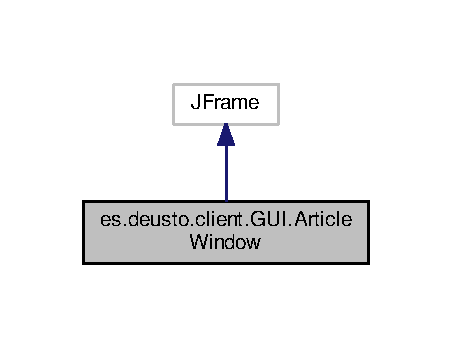
\includegraphics[width=217pt]{classes_1_1deusto_1_1client_1_1_g_u_i_1_1_article_window__inherit__graph}
\end{center}
\end{figure}


Collaboration diagram for es.\+deusto.\+client.\+G\+U\+I.\+Article\+Window\+:
\nopagebreak
\begin{figure}[H]
\begin{center}
\leavevmode
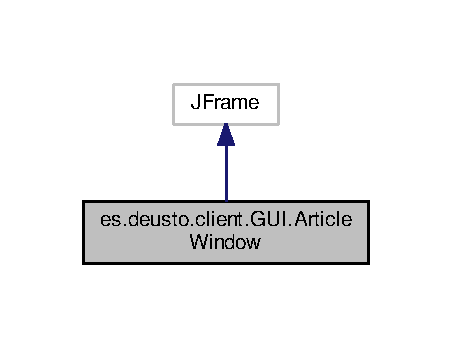
\includegraphics[width=217pt]{classes_1_1deusto_1_1client_1_1_g_u_i_1_1_article_window__coll__graph}
\end{center}
\end{figure}
\subsection*{Public Member Functions}
\begin{DoxyCompactItemize}
\item 
\hyperlink{classes_1_1deusto_1_1client_1_1_g_u_i_1_1_article_window_a32785c5a8d12fccb60c87c7dacf53e7f}{Article\+Window} ()
\end{DoxyCompactItemize}


\subsection{Detailed Description}


Definition at line 10 of file Article\+Window.\+java.



\subsection{Constructor \& Destructor Documentation}
\mbox{\Hypertarget{classes_1_1deusto_1_1client_1_1_g_u_i_1_1_article_window_a32785c5a8d12fccb60c87c7dacf53e7f}\label{classes_1_1deusto_1_1client_1_1_g_u_i_1_1_article_window_a32785c5a8d12fccb60c87c7dacf53e7f}} 
\index{es\+::deusto\+::client\+::\+G\+U\+I\+::\+Article\+Window@{es\+::deusto\+::client\+::\+G\+U\+I\+::\+Article\+Window}!Article\+Window@{Article\+Window}}
\index{Article\+Window@{Article\+Window}!es\+::deusto\+::client\+::\+G\+U\+I\+::\+Article\+Window@{es\+::deusto\+::client\+::\+G\+U\+I\+::\+Article\+Window}}
\subsubsection{\texorpdfstring{Article\+Window()}{ArticleWindow()}}
{\footnotesize\ttfamily es.\+deusto.\+client.\+G\+U\+I.\+Article\+Window.\+Article\+Window (\begin{DoxyParamCaption}{ }\end{DoxyParamCaption})}



Definition at line 12 of file Article\+Window.\+java.



The documentation for this class was generated from the following file\+:\begin{DoxyCompactItemize}
\item 
src/main/java/es/deusto/client/\+G\+U\+I/\hyperlink{_article_window_8java}{Article\+Window.\+java}\end{DoxyCompactItemize}

\hypertarget{classes_1_1deusto_1_1client_1_1_client}{}\section{es.\+deusto.\+client.\+Client Class Reference}
\label{classes_1_1deusto_1_1client_1_1_client}\index{es.\+deusto.\+client.\+Client@{es.\+deusto.\+client.\+Client}}


Collaboration diagram for es.\+deusto.\+client.\+Client\+:\nopagebreak
\begin{figure}[H]
\begin{center}
\leavevmode
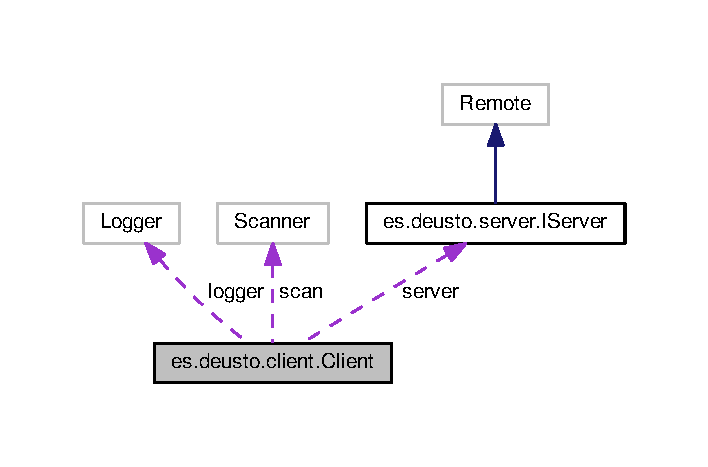
\includegraphics[width=340pt]{classes_1_1deusto_1_1client_1_1_client__coll__graph}
\end{center}
\end{figure}
\subsection*{Public Member Functions}
\begin{DoxyCompactItemize}
\item 
void \hyperlink{classes_1_1deusto_1_1client_1_1_client_a7a7fe3b9a2360883bd7697efe69816dc}{connection} (String name)
\end{DoxyCompactItemize}
\subsection*{Static Public Member Functions}
\begin{DoxyCompactItemize}
\item 
static void \hyperlink{classes_1_1deusto_1_1client_1_1_client_a69a7526d0af9cb2341f4bf341b501152}{main} (String\mbox{[}$\,$\mbox{]} args)
\end{DoxyCompactItemize}
\subsection*{Protected Member Functions}
\begin{DoxyCompactItemize}
\item 
void \hyperlink{classes_1_1deusto_1_1client_1_1_client_a8fdee4eb01bf96421c91a0bc1fbdcb43}{menu} ()
\item 
void \hyperlink{classes_1_1deusto_1_1client_1_1_client_a1872e2d941c7f50c6cc13d80e8d28eef}{first\+Articles} ()  throws Remote\+Exception 
\item 
void \hyperlink{classes_1_1deusto_1_1client_1_1_client_a08731e01aee74e27a7a55ae48c636c84}{user\+Actions} ()  throws Remote\+Exception 
\item 
void \hyperlink{classes_1_1deusto_1_1client_1_1_client_aee57ed402853cda15cc53f102d6abf1c}{admin\+Actions} (\hyperlink{classes_1_1deusto_1_1server_1_1jdo_1_1_admin}{Admin} adm)  throws Remote\+Exception 
\end{DoxyCompactItemize}


\subsection{Detailed Description}
Hello world! 

Definition at line 25 of file Client.\+java.



\subsection{Member Function Documentation}
\mbox{\Hypertarget{classes_1_1deusto_1_1client_1_1_client_aee57ed402853cda15cc53f102d6abf1c}\label{classes_1_1deusto_1_1client_1_1_client_aee57ed402853cda15cc53f102d6abf1c}} 
\index{es\+::deusto\+::client\+::\+Client@{es\+::deusto\+::client\+::\+Client}!admin\+Actions@{admin\+Actions}}
\index{admin\+Actions@{admin\+Actions}!es\+::deusto\+::client\+::\+Client@{es\+::deusto\+::client\+::\+Client}}
\subsubsection{\texorpdfstring{admin\+Actions()}{adminActions()}}
{\footnotesize\ttfamily void es.\+deusto.\+client.\+Client.\+admin\+Actions (\begin{DoxyParamCaption}\item[{\hyperlink{classes_1_1deusto_1_1server_1_1jdo_1_1_admin}{Admin}}]{adm }\end{DoxyParamCaption}) throws Remote\+Exception\hspace{0.3cm}{\ttfamily [protected]}}



Definition at line 212 of file Client.\+java.

\mbox{\Hypertarget{classes_1_1deusto_1_1client_1_1_client_a7a7fe3b9a2360883bd7697efe69816dc}\label{classes_1_1deusto_1_1client_1_1_client_a7a7fe3b9a2360883bd7697efe69816dc}} 
\index{es\+::deusto\+::client\+::\+Client@{es\+::deusto\+::client\+::\+Client}!connection@{connection}}
\index{connection@{connection}!es\+::deusto\+::client\+::\+Client@{es\+::deusto\+::client\+::\+Client}}
\subsubsection{\texorpdfstring{connection()}{connection()}}
{\footnotesize\ttfamily void es.\+deusto.\+client.\+Client.\+connection (\begin{DoxyParamCaption}\item[{String}]{name }\end{DoxyParamCaption})}



Definition at line 49 of file Client.\+java.

\mbox{\Hypertarget{classes_1_1deusto_1_1client_1_1_client_a1872e2d941c7f50c6cc13d80e8d28eef}\label{classes_1_1deusto_1_1client_1_1_client_a1872e2d941c7f50c6cc13d80e8d28eef}} 
\index{es\+::deusto\+::client\+::\+Client@{es\+::deusto\+::client\+::\+Client}!first\+Articles@{first\+Articles}}
\index{first\+Articles@{first\+Articles}!es\+::deusto\+::client\+::\+Client@{es\+::deusto\+::client\+::\+Client}}
\subsubsection{\texorpdfstring{first\+Articles()}{firstArticles()}}
{\footnotesize\ttfamily void es.\+deusto.\+client.\+Client.\+first\+Articles (\begin{DoxyParamCaption}{ }\end{DoxyParamCaption}) throws Remote\+Exception\hspace{0.3cm}{\ttfamily [protected]}}



Definition at line 135 of file Client.\+java.

\mbox{\Hypertarget{classes_1_1deusto_1_1client_1_1_client_a69a7526d0af9cb2341f4bf341b501152}\label{classes_1_1deusto_1_1client_1_1_client_a69a7526d0af9cb2341f4bf341b501152}} 
\index{es\+::deusto\+::client\+::\+Client@{es\+::deusto\+::client\+::\+Client}!main@{main}}
\index{main@{main}!es\+::deusto\+::client\+::\+Client@{es\+::deusto\+::client\+::\+Client}}
\subsubsection{\texorpdfstring{main()}{main()}}
{\footnotesize\ttfamily static void es.\+deusto.\+client.\+Client.\+main (\begin{DoxyParamCaption}\item[{String \mbox{[}$\,$\mbox{]}}]{args }\end{DoxyParamCaption})\hspace{0.3cm}{\ttfamily [static]}}



Definition at line 30 of file Client.\+java.

\mbox{\Hypertarget{classes_1_1deusto_1_1client_1_1_client_a8fdee4eb01bf96421c91a0bc1fbdcb43}\label{classes_1_1deusto_1_1client_1_1_client_a8fdee4eb01bf96421c91a0bc1fbdcb43}} 
\index{es\+::deusto\+::client\+::\+Client@{es\+::deusto\+::client\+::\+Client}!menu@{menu}}
\index{menu@{menu}!es\+::deusto\+::client\+::\+Client@{es\+::deusto\+::client\+::\+Client}}
\subsubsection{\texorpdfstring{menu()}{menu()}}
{\footnotesize\ttfamily void es.\+deusto.\+client.\+Client.\+menu (\begin{DoxyParamCaption}{ }\end{DoxyParamCaption})\hspace{0.3cm}{\ttfamily [protected]}}



Definition at line 57 of file Client.\+java.

\mbox{\Hypertarget{classes_1_1deusto_1_1client_1_1_client_a08731e01aee74e27a7a55ae48c636c84}\label{classes_1_1deusto_1_1client_1_1_client_a08731e01aee74e27a7a55ae48c636c84}} 
\index{es\+::deusto\+::client\+::\+Client@{es\+::deusto\+::client\+::\+Client}!user\+Actions@{user\+Actions}}
\index{user\+Actions@{user\+Actions}!es\+::deusto\+::client\+::\+Client@{es\+::deusto\+::client\+::\+Client}}
\subsubsection{\texorpdfstring{user\+Actions()}{userActions()}}
{\footnotesize\ttfamily void es.\+deusto.\+client.\+Client.\+user\+Actions (\begin{DoxyParamCaption}{ }\end{DoxyParamCaption}) throws Remote\+Exception\hspace{0.3cm}{\ttfamily [protected]}}



Definition at line 148 of file Client.\+java.



The documentation for this class was generated from the following file\+:\begin{DoxyCompactItemize}
\item 
/home/albertofdr/git/\+B\+S\+P\+Q19-\/\+E3/src/main/java/es/deusto/client/\hyperlink{_client_8java}{Client.\+java}\end{DoxyCompactItemize}

\hypertarget{classes_1_1deusto_1_1client_1_1_client_test}{}\section{es.\+deusto.\+client.\+Client\+Test Class Reference}
\label{classes_1_1deusto_1_1client_1_1_client_test}\index{es.\+deusto.\+client.\+Client\+Test@{es.\+deusto.\+client.\+Client\+Test}}


Inheritance diagram for es.\+deusto.\+client.\+Client\+Test\+:\nopagebreak
\begin{figure}[H]
\begin{center}
\leavevmode
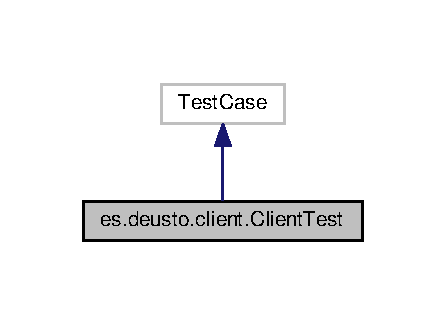
\includegraphics[width=214pt]{classes_1_1deusto_1_1client_1_1_client_test__inherit__graph}
\end{center}
\end{figure}


Collaboration diagram for es.\+deusto.\+client.\+Client\+Test\+:\nopagebreak
\begin{figure}[H]
\begin{center}
\leavevmode
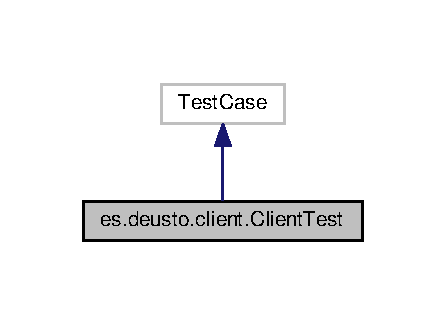
\includegraphics[width=214pt]{classes_1_1deusto_1_1client_1_1_client_test__coll__graph}
\end{center}
\end{figure}
\subsection*{Public Member Functions}
\begin{DoxyCompactItemize}
\item 
\hyperlink{classes_1_1deusto_1_1client_1_1_client_test_a452050f3521bf56054ec20630a137e02}{Client\+Test} (String test\+Name)
\item 
void \hyperlink{classes_1_1deusto_1_1client_1_1_client_test_af869b513820b21f952c9754d3aea8d97}{test\+App} ()  throws Remote\+Exception 
\end{DoxyCompactItemize}
\subsection*{Static Public Member Functions}
\begin{DoxyCompactItemize}
\item 
static Test \hyperlink{classes_1_1deusto_1_1client_1_1_client_test_a722a329c5978bafaf821de257fc762c8}{suite} ()
\end{DoxyCompactItemize}


\subsection{Detailed Description}
Unit test for simple App. 

Definition at line 13 of file Client\+Test.\+java.



\subsection{Constructor \& Destructor Documentation}
\mbox{\Hypertarget{classes_1_1deusto_1_1client_1_1_client_test_a452050f3521bf56054ec20630a137e02}\label{classes_1_1deusto_1_1client_1_1_client_test_a452050f3521bf56054ec20630a137e02}} 
\index{es\+::deusto\+::client\+::\+Client\+Test@{es\+::deusto\+::client\+::\+Client\+Test}!Client\+Test@{Client\+Test}}
\index{Client\+Test@{Client\+Test}!es\+::deusto\+::client\+::\+Client\+Test@{es\+::deusto\+::client\+::\+Client\+Test}}
\subsubsection{\texorpdfstring{Client\+Test()}{ClientTest()}}
{\footnotesize\ttfamily es.\+deusto.\+client.\+Client\+Test.\+Client\+Test (\begin{DoxyParamCaption}\item[{String}]{test\+Name }\end{DoxyParamCaption})}

Create the test case


\begin{DoxyParams}{Parameters}
{\em test\+Name} & name of the test case \\
\hline
\end{DoxyParams}


Definition at line 21 of file Client\+Test.\+java.



\subsection{Member Function Documentation}
\mbox{\Hypertarget{classes_1_1deusto_1_1client_1_1_client_test_a722a329c5978bafaf821de257fc762c8}\label{classes_1_1deusto_1_1client_1_1_client_test_a722a329c5978bafaf821de257fc762c8}} 
\index{es\+::deusto\+::client\+::\+Client\+Test@{es\+::deusto\+::client\+::\+Client\+Test}!suite@{suite}}
\index{suite@{suite}!es\+::deusto\+::client\+::\+Client\+Test@{es\+::deusto\+::client\+::\+Client\+Test}}
\subsubsection{\texorpdfstring{suite()}{suite()}}
{\footnotesize\ttfamily static Test es.\+deusto.\+client.\+Client\+Test.\+suite (\begin{DoxyParamCaption}{ }\end{DoxyParamCaption})\hspace{0.3cm}{\ttfamily [static]}}

\begin{DoxyReturn}{Returns}
the suite of tests being tested 
\end{DoxyReturn}


Definition at line 29 of file Client\+Test.\+java.

\mbox{\Hypertarget{classes_1_1deusto_1_1client_1_1_client_test_af869b513820b21f952c9754d3aea8d97}\label{classes_1_1deusto_1_1client_1_1_client_test_af869b513820b21f952c9754d3aea8d97}} 
\index{es\+::deusto\+::client\+::\+Client\+Test@{es\+::deusto\+::client\+::\+Client\+Test}!test\+App@{test\+App}}
\index{test\+App@{test\+App}!es\+::deusto\+::client\+::\+Client\+Test@{es\+::deusto\+::client\+::\+Client\+Test}}
\subsubsection{\texorpdfstring{test\+App()}{testApp()}}
{\footnotesize\ttfamily void es.\+deusto.\+client.\+Client\+Test.\+test\+App (\begin{DoxyParamCaption}{ }\end{DoxyParamCaption}) throws Remote\+Exception}

Rigourous Test \+:-\/)


\begin{DoxyExceptions}{Exceptions}
{\em Remote\+Exception} & \\
\hline
\end{DoxyExceptions}


Definition at line 38 of file Client\+Test.\+java.



The documentation for this class was generated from the following file\+:\begin{DoxyCompactItemize}
\item 
/home/albertofdr/git/\+B\+S\+P\+Q19-\/\+E3/src/test/java/es/deusto/client/\hyperlink{_client_test_8java}{Client\+Test.\+java}\end{DoxyCompactItemize}

\hypertarget{classes_1_1deusto_1_1server_1_1jdo_1_1_d_b_test}{}\section{es.\+deusto.\+server.\+jdo.\+D\+B\+Test Class Reference}
\label{classes_1_1deusto_1_1server_1_1jdo_1_1_d_b_test}\index{es.\+deusto.\+server.\+jdo.\+D\+B\+Test@{es.\+deusto.\+server.\+jdo.\+D\+B\+Test}}


Collaboration diagram for es.\+deusto.\+server.\+jdo.\+D\+B\+Test\+:
\nopagebreak
\begin{figure}[H]
\begin{center}
\leavevmode
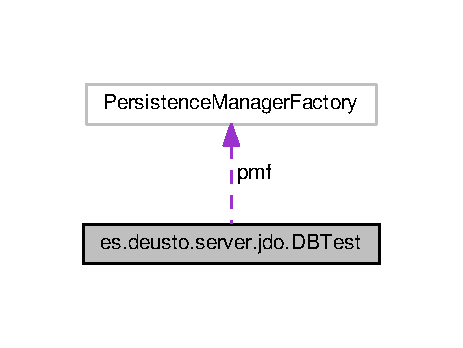
\includegraphics[width=222pt]{classes_1_1deusto_1_1server_1_1jdo_1_1_d_b_test__coll__graph}
\end{center}
\end{figure}
\subsection*{Static Public Member Functions}
\begin{DoxyCompactItemize}
\item 
static void \hyperlink{classes_1_1deusto_1_1server_1_1jdo_1_1_d_b_test_afd0180d9045ac006d8cbd145b9935c65}{main} (String args\mbox{[}$\,$\mbox{]})
\item 
static void \hyperlink{classes_1_1deusto_1_1server_1_1jdo_1_1_d_b_test_ae17f24746187cab1256b32c2b0ea1341}{delete\+DB} ()
\item 
static void \hyperlink{classes_1_1deusto_1_1server_1_1jdo_1_1_d_b_test_a8430b487bdfdf20d5f0e26517b7de1cc}{load\+DB} ()
\item 
static void \hyperlink{classes_1_1deusto_1_1server_1_1jdo_1_1_d_b_test_add160552e53376d7375c807043934688}{basic\+Test\+DB} ()
\end{DoxyCompactItemize}


\subsection{Detailed Description}


Definition at line 11 of file D\+B\+Test.\+java.



\subsection{Member Function Documentation}
\mbox{\Hypertarget{classes_1_1deusto_1_1server_1_1jdo_1_1_d_b_test_add160552e53376d7375c807043934688}\label{classes_1_1deusto_1_1server_1_1jdo_1_1_d_b_test_add160552e53376d7375c807043934688}} 
\index{es\+::deusto\+::server\+::jdo\+::\+D\+B\+Test@{es\+::deusto\+::server\+::jdo\+::\+D\+B\+Test}!basic\+Test\+DB@{basic\+Test\+DB}}
\index{basic\+Test\+DB@{basic\+Test\+DB}!es\+::deusto\+::server\+::jdo\+::\+D\+B\+Test@{es\+::deusto\+::server\+::jdo\+::\+D\+B\+Test}}
\subsubsection{\texorpdfstring{basic\+Test\+D\+B()}{basicTestDB()}}
{\footnotesize\ttfamily static void es.\+deusto.\+server.\+jdo.\+D\+B\+Test.\+basic\+Test\+DB (\begin{DoxyParamCaption}{ }\end{DoxyParamCaption})\hspace{0.3cm}{\ttfamily [static]}}



Definition at line 103 of file D\+B\+Test.\+java.

\mbox{\Hypertarget{classes_1_1deusto_1_1server_1_1jdo_1_1_d_b_test_ae17f24746187cab1256b32c2b0ea1341}\label{classes_1_1deusto_1_1server_1_1jdo_1_1_d_b_test_ae17f24746187cab1256b32c2b0ea1341}} 
\index{es\+::deusto\+::server\+::jdo\+::\+D\+B\+Test@{es\+::deusto\+::server\+::jdo\+::\+D\+B\+Test}!delete\+DB@{delete\+DB}}
\index{delete\+DB@{delete\+DB}!es\+::deusto\+::server\+::jdo\+::\+D\+B\+Test@{es\+::deusto\+::server\+::jdo\+::\+D\+B\+Test}}
\subsubsection{\texorpdfstring{delete\+D\+B()}{deleteDB()}}
{\footnotesize\ttfamily static void es.\+deusto.\+server.\+jdo.\+D\+B\+Test.\+delete\+DB (\begin{DoxyParamCaption}{ }\end{DoxyParamCaption})\hspace{0.3cm}{\ttfamily [static]}}



Definition at line 26 of file D\+B\+Test.\+java.

\mbox{\Hypertarget{classes_1_1deusto_1_1server_1_1jdo_1_1_d_b_test_a8430b487bdfdf20d5f0e26517b7de1cc}\label{classes_1_1deusto_1_1server_1_1jdo_1_1_d_b_test_a8430b487bdfdf20d5f0e26517b7de1cc}} 
\index{es\+::deusto\+::server\+::jdo\+::\+D\+B\+Test@{es\+::deusto\+::server\+::jdo\+::\+D\+B\+Test}!load\+DB@{load\+DB}}
\index{load\+DB@{load\+DB}!es\+::deusto\+::server\+::jdo\+::\+D\+B\+Test@{es\+::deusto\+::server\+::jdo\+::\+D\+B\+Test}}
\subsubsection{\texorpdfstring{load\+D\+B()}{loadDB()}}
{\footnotesize\ttfamily static void es.\+deusto.\+server.\+jdo.\+D\+B\+Test.\+load\+DB (\begin{DoxyParamCaption}{ }\end{DoxyParamCaption})\hspace{0.3cm}{\ttfamily [static]}}



Definition at line 57 of file D\+B\+Test.\+java.

\mbox{\Hypertarget{classes_1_1deusto_1_1server_1_1jdo_1_1_d_b_test_afd0180d9045ac006d8cbd145b9935c65}\label{classes_1_1deusto_1_1server_1_1jdo_1_1_d_b_test_afd0180d9045ac006d8cbd145b9935c65}} 
\index{es\+::deusto\+::server\+::jdo\+::\+D\+B\+Test@{es\+::deusto\+::server\+::jdo\+::\+D\+B\+Test}!main@{main}}
\index{main@{main}!es\+::deusto\+::server\+::jdo\+::\+D\+B\+Test@{es\+::deusto\+::server\+::jdo\+::\+D\+B\+Test}}
\subsubsection{\texorpdfstring{main()}{main()}}
{\footnotesize\ttfamily static void es.\+deusto.\+server.\+jdo.\+D\+B\+Test.\+main (\begin{DoxyParamCaption}\item[{String}]{args\mbox{[}$\,$\mbox{]} }\end{DoxyParamCaption})\hspace{0.3cm}{\ttfamily [static]}}



Definition at line 14 of file D\+B\+Test.\+java.



The documentation for this class was generated from the following file\+:\begin{DoxyCompactItemize}
\item 
src/main/java/es/deusto/server/jdo/\hyperlink{_d_b_test_8java}{D\+B\+Test.\+java}\end{DoxyCompactItemize}

\hypertarget{interfacees_1_1deusto_1_1server_1_1_i_server}{}\section{es.\+deusto.\+server.\+I\+Server Interface Reference}
\label{interfacees_1_1deusto_1_1server_1_1_i_server}\index{es.\+deusto.\+server.\+I\+Server@{es.\+deusto.\+server.\+I\+Server}}


Inheritance diagram for es.\+deusto.\+server.\+I\+Server\+:\nopagebreak
\begin{figure}[H]
\begin{center}
\leavevmode
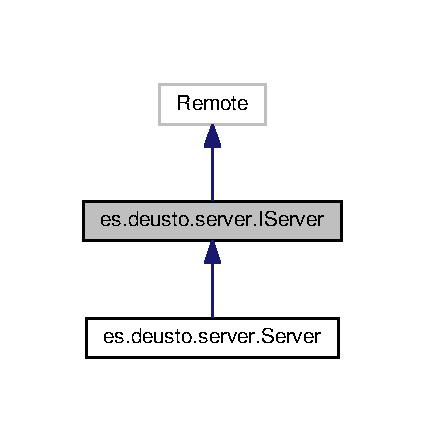
\includegraphics[width=204pt]{interfacees_1_1deusto_1_1server_1_1_i_server__inherit__graph}
\end{center}
\end{figure}


Collaboration diagram for es.\+deusto.\+server.\+I\+Server\+:\nopagebreak
\begin{figure}[H]
\begin{center}
\leavevmode
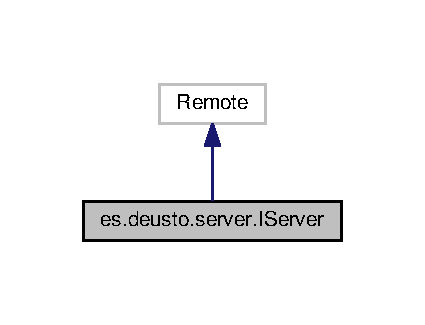
\includegraphics[width=204pt]{interfacees_1_1deusto_1_1server_1_1_i_server__coll__graph}
\end{center}
\end{figure}
\subsection*{Public Member Functions}
\begin{DoxyCompactItemize}
\item 
Boolean \hyperlink{interfacees_1_1deusto_1_1server_1_1_i_server_a3b0fbbc1c934b8e527ecfed69e497155}{register\+User} (String login, String password, String email)  throws Remote\+Exception
\item 
\hyperlink{classes_1_1deusto_1_1server_1_1jdo_1_1_user}{User} \hyperlink{interfacees_1_1deusto_1_1server_1_1_i_server_ae6b27c8714c2e2eadc9a55bccb0543fc}{log\+In} (String user, String pass)  throws Remote\+Exception
\item 
\hyperlink{classes_1_1deusto_1_1server_1_1jdo_1_1_admin}{Admin} \hyperlink{interfacees_1_1deusto_1_1server_1_1_i_server_a65588c309522410e6a6d9c27d80821a7}{log\+In\+Admin} (String user, String pass)  throws Remote\+Exception
\item 
\hyperlink{classes_1_1deusto_1_1server_1_1jdo_1_1_article}{Article} \hyperlink{interfacees_1_1deusto_1_1server_1_1_i_server_a1f02a5aa0628909b5464141923f5d1d2}{read\+Article} (String title)  throws Remote\+Exception
\item 
Boolean \hyperlink{interfacees_1_1deusto_1_1server_1_1_i_server_a74b3203c5a8d94e91004df0dc84ca386}{create\+Article} (\hyperlink{classes_1_1deusto_1_1server_1_1jdo_1_1_article}{Article} art, \hyperlink{classes_1_1deusto_1_1server_1_1jdo_1_1_admin}{Admin} author)  throws Remote\+Exception
\item 
Array\+List$<$ \hyperlink{classes_1_1deusto_1_1server_1_1jdo_1_1_article}{Article} $>$ \hyperlink{interfacees_1_1deusto_1_1server_1_1_i_server_ab08ccd2295e983571cf50431d273393a}{search\+Article\+Category} (String category)  throws Remote\+Exception
\item 
Array\+List$<$ \hyperlink{classes_1_1deusto_1_1server_1_1jdo_1_1_article}{Article} $>$ \hyperlink{interfacees_1_1deusto_1_1server_1_1_i_server_a92b587f25a7043b24d44f326d1c7b7ae}{search\+Article\+Author} (String author)  throws Remote\+Exception
\item 
Boolean \hyperlink{interfacees_1_1deusto_1_1server_1_1_i_server_ac96e072eb8a660ebcd5e535cb1324e64}{delete\+Article} (\hyperlink{classes_1_1deusto_1_1server_1_1jdo_1_1_article}{Article} art, \hyperlink{classes_1_1deusto_1_1server_1_1jdo_1_1_admin}{Admin} autho)  throws Remote\+Exception
\item 
Boolean \hyperlink{interfacees_1_1deusto_1_1server_1_1_i_server_ab5c4258f62146d90a064604891cedf2f}{edit\+Article} (\hyperlink{classes_1_1deusto_1_1server_1_1jdo_1_1_article}{Article} e, String new\+Title, String new\+Body, \hyperlink{classes_1_1deusto_1_1server_1_1jdo_1_1_admin}{Admin} autho)  throws Remote\+Exception
\item 
Array\+List$<$ \hyperlink{classes_1_1deusto_1_1server_1_1jdo_1_1_article}{Article} $>$ \hyperlink{interfacees_1_1deusto_1_1server_1_1_i_server_ab1b33472017b55ae84bf849430db5f1b}{view\+Top\+Article} ()  throws Remote\+Exception
\item 
Array\+List$<$ \hyperlink{classes_1_1deusto_1_1server_1_1jdo_1_1_article}{Article} $>$ \hyperlink{interfacees_1_1deusto_1_1server_1_1_i_server_a27b2a5526387404d63d7fc6d0415acd4}{get\+First\+Articles} ()  throws Remote\+Exception
\end{DoxyCompactItemize}


\subsection{Detailed Description}


Definition at line 16 of file I\+Server.\+java.



\subsection{Member Function Documentation}
\mbox{\Hypertarget{interfacees_1_1deusto_1_1server_1_1_i_server_a74b3203c5a8d94e91004df0dc84ca386}\label{interfacees_1_1deusto_1_1server_1_1_i_server_a74b3203c5a8d94e91004df0dc84ca386}} 
\index{es\+::deusto\+::server\+::\+I\+Server@{es\+::deusto\+::server\+::\+I\+Server}!create\+Article@{create\+Article}}
\index{create\+Article@{create\+Article}!es\+::deusto\+::server\+::\+I\+Server@{es\+::deusto\+::server\+::\+I\+Server}}
\subsubsection{\texorpdfstring{create\+Article()}{createArticle()}}
{\footnotesize\ttfamily Boolean es.\+deusto.\+server.\+I\+Server.\+create\+Article (\begin{DoxyParamCaption}\item[{\hyperlink{classes_1_1deusto_1_1server_1_1jdo_1_1_article}{Article}}]{art,  }\item[{\hyperlink{classes_1_1deusto_1_1server_1_1jdo_1_1_admin}{Admin}}]{author }\end{DoxyParamCaption}) throws Remote\+Exception}

To create an article


\begin{DoxyParams}{Parameters}
{\em Article} & the article to create \\
\hline
{\em Admin} & the admin that is creating the article \\
\hline
\end{DoxyParams}
\begin{DoxyReturn}{Returns}
boolean true(created) false(not created) 
\end{DoxyReturn}


Implemented in \hyperlink{classes_1_1deusto_1_1server_1_1_server_a58363d9c2c5c5d1e085e22deeeebf833}{es.\+deusto.\+server.\+Server}.

\mbox{\Hypertarget{interfacees_1_1deusto_1_1server_1_1_i_server_ac96e072eb8a660ebcd5e535cb1324e64}\label{interfacees_1_1deusto_1_1server_1_1_i_server_ac96e072eb8a660ebcd5e535cb1324e64}} 
\index{es\+::deusto\+::server\+::\+I\+Server@{es\+::deusto\+::server\+::\+I\+Server}!delete\+Article@{delete\+Article}}
\index{delete\+Article@{delete\+Article}!es\+::deusto\+::server\+::\+I\+Server@{es\+::deusto\+::server\+::\+I\+Server}}
\subsubsection{\texorpdfstring{delete\+Article()}{deleteArticle()}}
{\footnotesize\ttfamily Boolean es.\+deusto.\+server.\+I\+Server.\+delete\+Article (\begin{DoxyParamCaption}\item[{\hyperlink{classes_1_1deusto_1_1server_1_1jdo_1_1_article}{Article}}]{art,  }\item[{\hyperlink{classes_1_1deusto_1_1server_1_1jdo_1_1_admin}{Admin}}]{autho }\end{DoxyParamCaption}) throws Remote\+Exception}

To delete an existing article


\begin{DoxyParams}{Parameters}
{\em Article,the} & one to be deleted that must be searched in the db \\
\hline
{\em Admin,the} & one that is deleting the article \\
\hline
\end{DoxyParams}
\begin{DoxyReturn}{Returns}
boolean true(deleted) false(not deleted) 
\end{DoxyReturn}


Implemented in \hyperlink{classes_1_1deusto_1_1server_1_1_server_ad9d8810833b631866924dc481801614a}{es.\+deusto.\+server.\+Server}.

\mbox{\Hypertarget{interfacees_1_1deusto_1_1server_1_1_i_server_ab5c4258f62146d90a064604891cedf2f}\label{interfacees_1_1deusto_1_1server_1_1_i_server_ab5c4258f62146d90a064604891cedf2f}} 
\index{es\+::deusto\+::server\+::\+I\+Server@{es\+::deusto\+::server\+::\+I\+Server}!edit\+Article@{edit\+Article}}
\index{edit\+Article@{edit\+Article}!es\+::deusto\+::server\+::\+I\+Server@{es\+::deusto\+::server\+::\+I\+Server}}
\subsubsection{\texorpdfstring{edit\+Article()}{editArticle()}}
{\footnotesize\ttfamily Boolean es.\+deusto.\+server.\+I\+Server.\+edit\+Article (\begin{DoxyParamCaption}\item[{\hyperlink{classes_1_1deusto_1_1server_1_1jdo_1_1_article}{Article}}]{e,  }\item[{String}]{new\+Title,  }\item[{String}]{new\+Body,  }\item[{\hyperlink{classes_1_1deusto_1_1server_1_1jdo_1_1_admin}{Admin}}]{autho }\end{DoxyParamCaption}) throws Remote\+Exception}

To edit an article


\begin{DoxyParams}{Parameters}
{\em Article,the} & one to edit that must be searched in db \\
\hline
{\em String} & new\+Title, the new title that must be given to the article \\
\hline
{\em boolean} & change\+Title, whether the title must be changed or not \\
\hline
{\em String} & new\+Body, the new body that must be given to the article \\
\hline
{\em boolean} & change\+Body, whether the body must be changed or not \\
\hline
{\em Admin,the} & one that is editing the article \\
\hline
\end{DoxyParams}
\begin{DoxyReturn}{Returns}
boolean true(edited) false(not edited) 
\end{DoxyReturn}


Implemented in \hyperlink{classes_1_1deusto_1_1server_1_1_server_a2c4455392fb9fb404d425110b5905c6a}{es.\+deusto.\+server.\+Server}.

\mbox{\Hypertarget{interfacees_1_1deusto_1_1server_1_1_i_server_a27b2a5526387404d63d7fc6d0415acd4}\label{interfacees_1_1deusto_1_1server_1_1_i_server_a27b2a5526387404d63d7fc6d0415acd4}} 
\index{es\+::deusto\+::server\+::\+I\+Server@{es\+::deusto\+::server\+::\+I\+Server}!get\+First\+Articles@{get\+First\+Articles}}
\index{get\+First\+Articles@{get\+First\+Articles}!es\+::deusto\+::server\+::\+I\+Server@{es\+::deusto\+::server\+::\+I\+Server}}
\subsubsection{\texorpdfstring{get\+First\+Articles()}{getFirstArticles()}}
{\footnotesize\ttfamily Array\+List$<$\hyperlink{classes_1_1deusto_1_1server_1_1jdo_1_1_article}{Article}$>$ es.\+deusto.\+server.\+I\+Server.\+get\+First\+Articles (\begin{DoxyParamCaption}{ }\end{DoxyParamCaption}) throws Remote\+Exception}

Returns the articles that see the user when enters

\begin{DoxyReturn}{Returns}
Array\+List$<$\+Article$>$ Returns the articles that the user will see in the timeline 
\end{DoxyReturn}


Implemented in \hyperlink{classes_1_1deusto_1_1server_1_1_server_a64dfcee7821b0cc581367c1b21d9f97f}{es.\+deusto.\+server.\+Server}.

\mbox{\Hypertarget{interfacees_1_1deusto_1_1server_1_1_i_server_ae6b27c8714c2e2eadc9a55bccb0543fc}\label{interfacees_1_1deusto_1_1server_1_1_i_server_ae6b27c8714c2e2eadc9a55bccb0543fc}} 
\index{es\+::deusto\+::server\+::\+I\+Server@{es\+::deusto\+::server\+::\+I\+Server}!log\+In@{log\+In}}
\index{log\+In@{log\+In}!es\+::deusto\+::server\+::\+I\+Server@{es\+::deusto\+::server\+::\+I\+Server}}
\subsubsection{\texorpdfstring{log\+In()}{logIn()}}
{\footnotesize\ttfamily \hyperlink{classes_1_1deusto_1_1server_1_1jdo_1_1_user}{User} es.\+deusto.\+server.\+I\+Server.\+log\+In (\begin{DoxyParamCaption}\item[{String}]{user,  }\item[{String}]{pass }\end{DoxyParamCaption}) throws Remote\+Exception}

To log in a U\+S\+ER


\begin{DoxyParams}{Parameters}
{\em user} & The username of the person \\
\hline
{\em pass} & the p logger.\+info(\char`\"{}-\/-\/-\/\+The article does not exist in the db, so it
            cannot be edited-\/-\/-\/\char`\"{}); assword of that person \\
\hline
\end{DoxyParams}
\begin{DoxyReturn}{Returns}
Returns the user of that person 
\end{DoxyReturn}


Implemented in \hyperlink{classes_1_1deusto_1_1server_1_1_server_a5a570da0fbfec7afdf56bd3648fc904f}{es.\+deusto.\+server.\+Server}.

\mbox{\Hypertarget{interfacees_1_1deusto_1_1server_1_1_i_server_a65588c309522410e6a6d9c27d80821a7}\label{interfacees_1_1deusto_1_1server_1_1_i_server_a65588c309522410e6a6d9c27d80821a7}} 
\index{es\+::deusto\+::server\+::\+I\+Server@{es\+::deusto\+::server\+::\+I\+Server}!log\+In\+Admin@{log\+In\+Admin}}
\index{log\+In\+Admin@{log\+In\+Admin}!es\+::deusto\+::server\+::\+I\+Server@{es\+::deusto\+::server\+::\+I\+Server}}
\subsubsection{\texorpdfstring{log\+In\+Admin()}{logInAdmin()}}
{\footnotesize\ttfamily \hyperlink{classes_1_1deusto_1_1server_1_1jdo_1_1_admin}{Admin} es.\+deusto.\+server.\+I\+Server.\+log\+In\+Admin (\begin{DoxyParamCaption}\item[{String}]{user,  }\item[{String}]{pass }\end{DoxyParamCaption}) throws Remote\+Exception}

To log in a A\+D\+M\+IN


\begin{DoxyParams}{Parameters}
{\em user} & The username of the person \\
\hline
{\em pass} & the password of that person \\
\hline
\end{DoxyParams}
\begin{DoxyReturn}{Returns}
Returns the admin of that person 
\end{DoxyReturn}


Implemented in \hyperlink{classes_1_1deusto_1_1server_1_1_server_a654d408d0865f8e3f2c931da9e90283a}{es.\+deusto.\+server.\+Server}.

\mbox{\Hypertarget{interfacees_1_1deusto_1_1server_1_1_i_server_a1f02a5aa0628909b5464141923f5d1d2}\label{interfacees_1_1deusto_1_1server_1_1_i_server_a1f02a5aa0628909b5464141923f5d1d2}} 
\index{es\+::deusto\+::server\+::\+I\+Server@{es\+::deusto\+::server\+::\+I\+Server}!read\+Article@{read\+Article}}
\index{read\+Article@{read\+Article}!es\+::deusto\+::server\+::\+I\+Server@{es\+::deusto\+::server\+::\+I\+Server}}
\subsubsection{\texorpdfstring{read\+Article()}{readArticle()}}
{\footnotesize\ttfamily \hyperlink{classes_1_1deusto_1_1server_1_1jdo_1_1_article}{Article} es.\+deusto.\+server.\+I\+Server.\+read\+Article (\begin{DoxyParamCaption}\item[{String}]{title }\end{DoxyParamCaption}) throws Remote\+Exception}

You send the title of an article which is the one that you want to read and returns the article. 
\begin{DoxyParams}{Parameters}
{\em String} & The title of the article \\
\hline
\end{DoxyParams}
\begin{DoxyReturn}{Returns}
Article Returns the article 
\end{DoxyReturn}


Implemented in \hyperlink{classes_1_1deusto_1_1server_1_1_server_ac3af6f09e37d0b86743f8f46e39acdad}{es.\+deusto.\+server.\+Server}.

\mbox{\Hypertarget{interfacees_1_1deusto_1_1server_1_1_i_server_a3b0fbbc1c934b8e527ecfed69e497155}\label{interfacees_1_1deusto_1_1server_1_1_i_server_a3b0fbbc1c934b8e527ecfed69e497155}} 
\index{es\+::deusto\+::server\+::\+I\+Server@{es\+::deusto\+::server\+::\+I\+Server}!register\+User@{register\+User}}
\index{register\+User@{register\+User}!es\+::deusto\+::server\+::\+I\+Server@{es\+::deusto\+::server\+::\+I\+Server}}
\subsubsection{\texorpdfstring{register\+User()}{registerUser()}}
{\footnotesize\ttfamily Boolean es.\+deusto.\+server.\+I\+Server.\+register\+User (\begin{DoxyParamCaption}\item[{String}]{login,  }\item[{String}]{password,  }\item[{String}]{email }\end{DoxyParamCaption}) throws Remote\+Exception}

Register a user in the DB


\begin{DoxyParams}{Parameters}
{\em login} & The username of the person \\
\hline
{\em password} & The password of the person \\
\hline
{\em email} & The email of the person \\
\hline
\end{DoxyParams}
\begin{DoxyReturn}{Returns}
Returns a Boolean, if the transaction works well returns true 
\end{DoxyReturn}


Implemented in \hyperlink{classes_1_1deusto_1_1server_1_1_server_a0ab63e5bc49a52ff84f7d6859161b683}{es.\+deusto.\+server.\+Server}.

\mbox{\Hypertarget{interfacees_1_1deusto_1_1server_1_1_i_server_a92b587f25a7043b24d44f326d1c7b7ae}\label{interfacees_1_1deusto_1_1server_1_1_i_server_a92b587f25a7043b24d44f326d1c7b7ae}} 
\index{es\+::deusto\+::server\+::\+I\+Server@{es\+::deusto\+::server\+::\+I\+Server}!search\+Article\+Author@{search\+Article\+Author}}
\index{search\+Article\+Author@{search\+Article\+Author}!es\+::deusto\+::server\+::\+I\+Server@{es\+::deusto\+::server\+::\+I\+Server}}
\subsubsection{\texorpdfstring{search\+Article\+Author()}{searchArticleAuthor()}}
{\footnotesize\ttfamily Array\+List$<$\hyperlink{classes_1_1deusto_1_1server_1_1jdo_1_1_article}{Article}$>$ es.\+deusto.\+server.\+I\+Server.\+search\+Article\+Author (\begin{DoxyParamCaption}\item[{String}]{author }\end{DoxyParamCaption}) throws Remote\+Exception}

Search the articles of one author 
\begin{DoxyParams}{Parameters}
{\em String} & The name of the author we want to read \\
\hline
\end{DoxyParams}
\begin{DoxyReturn}{Returns}
Array\+List$<$\+Article$>$ returns the list of articles of that author 
\end{DoxyReturn}


Implemented in \hyperlink{classes_1_1deusto_1_1server_1_1_server_a5f04113ce0c895e13e1bde76d7b41eb8}{es.\+deusto.\+server.\+Server}.

\mbox{\Hypertarget{interfacees_1_1deusto_1_1server_1_1_i_server_ab08ccd2295e983571cf50431d273393a}\label{interfacees_1_1deusto_1_1server_1_1_i_server_ab08ccd2295e983571cf50431d273393a}} 
\index{es\+::deusto\+::server\+::\+I\+Server@{es\+::deusto\+::server\+::\+I\+Server}!search\+Article\+Category@{search\+Article\+Category}}
\index{search\+Article\+Category@{search\+Article\+Category}!es\+::deusto\+::server\+::\+I\+Server@{es\+::deusto\+::server\+::\+I\+Server}}
\subsubsection{\texorpdfstring{search\+Article\+Category()}{searchArticleCategory()}}
{\footnotesize\ttfamily Array\+List$<$\hyperlink{classes_1_1deusto_1_1server_1_1jdo_1_1_article}{Article}$>$ es.\+deusto.\+server.\+I\+Server.\+search\+Article\+Category (\begin{DoxyParamCaption}\item[{String}]{category }\end{DoxyParamCaption}) throws Remote\+Exception}

Search the articles which have one category 
\begin{DoxyParams}{Parameters}
{\em String} & The category we want to read \\
\hline
\end{DoxyParams}
\begin{DoxyReturn}{Returns}
Array\+List$<$\+Article$>$ returns the list of articles with that category 
\end{DoxyReturn}


Implemented in \hyperlink{classes_1_1deusto_1_1server_1_1_server_ab2729689bb71bd707881b563cdf2a006}{es.\+deusto.\+server.\+Server}.

\mbox{\Hypertarget{interfacees_1_1deusto_1_1server_1_1_i_server_ab1b33472017b55ae84bf849430db5f1b}\label{interfacees_1_1deusto_1_1server_1_1_i_server_ab1b33472017b55ae84bf849430db5f1b}} 
\index{es\+::deusto\+::server\+::\+I\+Server@{es\+::deusto\+::server\+::\+I\+Server}!view\+Top\+Article@{view\+Top\+Article}}
\index{view\+Top\+Article@{view\+Top\+Article}!es\+::deusto\+::server\+::\+I\+Server@{es\+::deusto\+::server\+::\+I\+Server}}
\subsubsection{\texorpdfstring{view\+Top\+Article()}{viewTopArticle()}}
{\footnotesize\ttfamily Array\+List$<$\hyperlink{classes_1_1deusto_1_1server_1_1jdo_1_1_article}{Article}$>$ es.\+deusto.\+server.\+I\+Server.\+view\+Top\+Article (\begin{DoxyParamCaption}{ }\end{DoxyParamCaption}) throws Remote\+Exception}

A method which search the most visited articles \begin{DoxyReturn}{Returns}
Array\+List$<$\+Article$>$ returns the top articles 
\end{DoxyReturn}


Implemented in \hyperlink{classes_1_1deusto_1_1server_1_1_server_ada6d55bcd79444de821eaeb6b21c44b8}{es.\+deusto.\+server.\+Server}.



The documentation for this interface was generated from the following file\+:\begin{DoxyCompactItemize}
\item 
/home/albertofdr/git/\+B\+S\+P\+Q19-\/\+E3/src/main/java/es/deusto/server/\hyperlink{_i_server_8java}{I\+Server.\+java}\end{DoxyCompactItemize}

\hypertarget{classes_1_1deusto_1_1client_1_1_g_u_i_1_1_login_window_user}{}\section{es.\+deusto.\+client.\+G\+U\+I.\+Login\+Window\+User Class Reference}
\label{classes_1_1deusto_1_1client_1_1_g_u_i_1_1_login_window_user}\index{es.\+deusto.\+client.\+G\+U\+I.\+Login\+Window\+User@{es.\+deusto.\+client.\+G\+U\+I.\+Login\+Window\+User}}


Inheritance diagram for es.\+deusto.\+client.\+G\+U\+I.\+Login\+Window\+User\+:\nopagebreak
\begin{figure}[H]
\begin{center}
\leavevmode
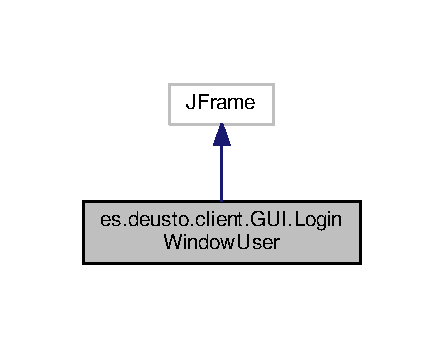
\includegraphics[width=213pt]{classes_1_1deusto_1_1client_1_1_g_u_i_1_1_login_window_user__inherit__graph}
\end{center}
\end{figure}


Collaboration diagram for es.\+deusto.\+client.\+G\+U\+I.\+Login\+Window\+User\+:\nopagebreak
\begin{figure}[H]
\begin{center}
\leavevmode
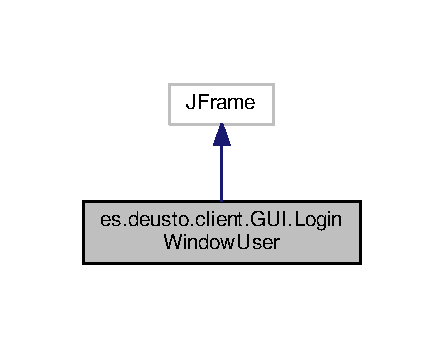
\includegraphics[width=213pt]{classes_1_1deusto_1_1client_1_1_g_u_i_1_1_login_window_user__coll__graph}
\end{center}
\end{figure}
\subsection*{Public Member Functions}
\begin{DoxyCompactItemize}
\item 
\hyperlink{classes_1_1deusto_1_1client_1_1_g_u_i_1_1_login_window_user_a616579d965d1677e6956a864a944ee87}{Login\+Window\+User} (\hyperlink{classes_1_1deusto_1_1client_1_1_g_u_i_1_1_main_window}{Main\+Window} main\+Window, int tipo)
\end{DoxyCompactItemize}


\subsection{Detailed Description}


Definition at line 30 of file Login\+Window\+User.\+java.



\subsection{Constructor \& Destructor Documentation}
\mbox{\Hypertarget{classes_1_1deusto_1_1client_1_1_g_u_i_1_1_login_window_user_a616579d965d1677e6956a864a944ee87}\label{classes_1_1deusto_1_1client_1_1_g_u_i_1_1_login_window_user_a616579d965d1677e6956a864a944ee87}} 
\index{es\+::deusto\+::client\+::\+G\+U\+I\+::\+Login\+Window\+User@{es\+::deusto\+::client\+::\+G\+U\+I\+::\+Login\+Window\+User}!Login\+Window\+User@{Login\+Window\+User}}
\index{Login\+Window\+User@{Login\+Window\+User}!es\+::deusto\+::client\+::\+G\+U\+I\+::\+Login\+Window\+User@{es\+::deusto\+::client\+::\+G\+U\+I\+::\+Login\+Window\+User}}
\subsubsection{\texorpdfstring{Login\+Window\+User()}{LoginWindowUser()}}
{\footnotesize\ttfamily es.\+deusto.\+client.\+G\+U\+I.\+Login\+Window\+User.\+Login\+Window\+User (\begin{DoxyParamCaption}\item[{\hyperlink{classes_1_1deusto_1_1client_1_1_g_u_i_1_1_main_window}{Main\+Window}}]{main\+Window,  }\item[{int}]{tipo }\end{DoxyParamCaption})}



Definition at line 36 of file Login\+Window\+User.\+java.



The documentation for this class was generated from the following file\+:\begin{DoxyCompactItemize}
\item 
/home/albertofdr/git/\+B\+S\+P\+Q19-\/\+E3/src/main/java/es/deusto/client/\+G\+U\+I/\hyperlink{_login_window_user_8java}{Login\+Window\+User.\+java}\end{DoxyCompactItemize}

\hypertarget{classes_1_1deusto_1_1client_1_1_g_u_i_1_1_main_window}{}\section{es.\+deusto.\+client.\+G\+U\+I.\+Main\+Window Class Reference}
\label{classes_1_1deusto_1_1client_1_1_g_u_i_1_1_main_window}\index{es.\+deusto.\+client.\+G\+U\+I.\+Main\+Window@{es.\+deusto.\+client.\+G\+U\+I.\+Main\+Window}}


Inheritance diagram for es.\+deusto.\+client.\+G\+U\+I.\+Main\+Window\+:
\nopagebreak
\begin{figure}[H]
\begin{center}
\leavevmode
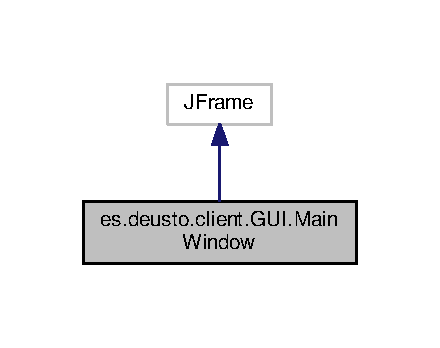
\includegraphics[width=211pt]{classes_1_1deusto_1_1client_1_1_g_u_i_1_1_main_window__inherit__graph}
\end{center}
\end{figure}


Collaboration diagram for es.\+deusto.\+client.\+G\+U\+I.\+Main\+Window\+:
\nopagebreak
\begin{figure}[H]
\begin{center}
\leavevmode
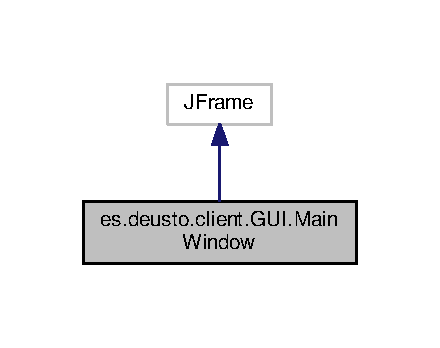
\includegraphics[width=211pt]{classes_1_1deusto_1_1client_1_1_g_u_i_1_1_main_window__coll__graph}
\end{center}
\end{figure}
\subsection*{Public Member Functions}
\begin{DoxyCompactItemize}
\item 
\hyperlink{classes_1_1deusto_1_1client_1_1_g_u_i_1_1_main_window_a471b4c0c749b9f22c1c74f85a410c1c9}{Main\+Window} ()
\end{DoxyCompactItemize}


\subsection{Detailed Description}


Definition at line 15 of file Main\+Window.\+java.



\subsection{Constructor \& Destructor Documentation}
\mbox{\Hypertarget{classes_1_1deusto_1_1client_1_1_g_u_i_1_1_main_window_a471b4c0c749b9f22c1c74f85a410c1c9}\label{classes_1_1deusto_1_1client_1_1_g_u_i_1_1_main_window_a471b4c0c749b9f22c1c74f85a410c1c9}} 
\index{es\+::deusto\+::client\+::\+G\+U\+I\+::\+Main\+Window@{es\+::deusto\+::client\+::\+G\+U\+I\+::\+Main\+Window}!Main\+Window@{Main\+Window}}
\index{Main\+Window@{Main\+Window}!es\+::deusto\+::client\+::\+G\+U\+I\+::\+Main\+Window@{es\+::deusto\+::client\+::\+G\+U\+I\+::\+Main\+Window}}
\subsubsection{\texorpdfstring{Main\+Window()}{MainWindow()}}
{\footnotesize\ttfamily es.\+deusto.\+client.\+G\+U\+I.\+Main\+Window.\+Main\+Window (\begin{DoxyParamCaption}{ }\end{DoxyParamCaption})}



Definition at line 19 of file Main\+Window.\+java.



The documentation for this class was generated from the following file\+:\begin{DoxyCompactItemize}
\item 
src/main/java/es/deusto/client/\+G\+U\+I/\hyperlink{_main_window_8java}{Main\+Window.\+java}\end{DoxyCompactItemize}

\hypertarget{classes_1_1deusto_1_1server_1_1_server}{}\section{es.\+deusto.\+server.\+Server Class Reference}
\label{classes_1_1deusto_1_1server_1_1_server}\index{es.\+deusto.\+server.\+Server@{es.\+deusto.\+server.\+Server}}


Inheritance diagram for es.\+deusto.\+server.\+Server\+:
\nopagebreak
\begin{figure}[H]
\begin{center}
\leavevmode
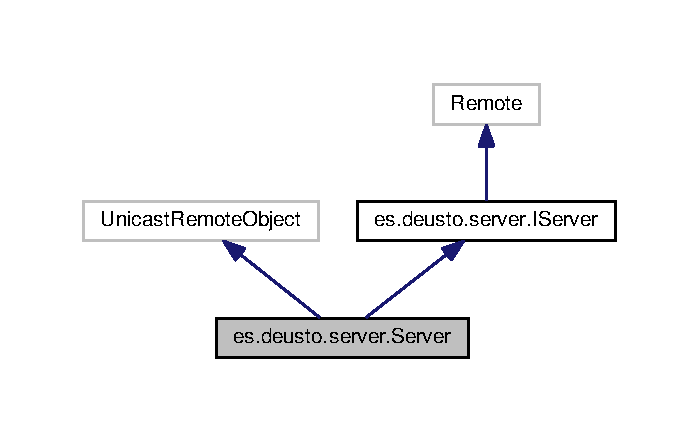
\includegraphics[width=336pt]{classes_1_1deusto_1_1server_1_1_server__inherit__graph}
\end{center}
\end{figure}


Collaboration diagram for es.\+deusto.\+server.\+Server\+:
\nopagebreak
\begin{figure}[H]
\begin{center}
\leavevmode
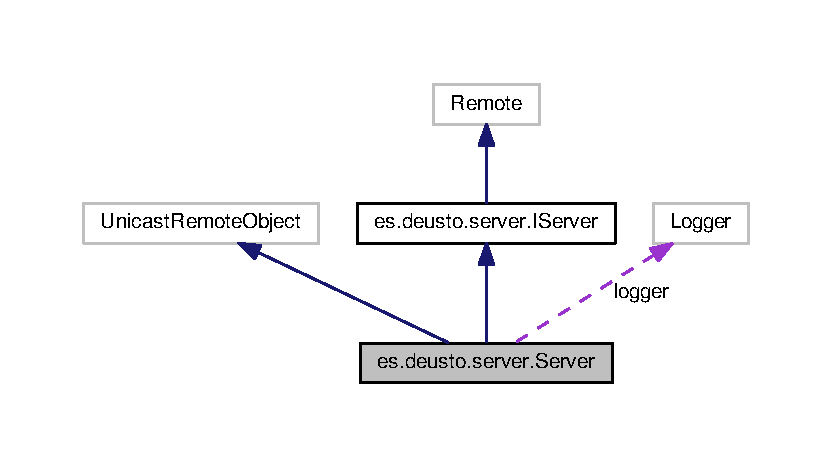
\includegraphics[width=350pt]{classes_1_1deusto_1_1server_1_1_server__coll__graph}
\end{center}
\end{figure}
\subsection*{Public Member Functions}
\begin{DoxyCompactItemize}
\item 
\hyperlink{classes_1_1deusto_1_1server_1_1_server_a84f78162a65dd737f224eb2f94c43023}{Server} ()  throws Remote\+Exception 
\item 
synchronized Boolean \hyperlink{classes_1_1deusto_1_1server_1_1_server_a0ab63e5bc49a52ff84f7d6859161b683}{register\+User} (String login, String password, String email)  throws Remote\+Exception 
\item 
synchronized \hyperlink{classes_1_1deusto_1_1server_1_1jdo_1_1_user}{User} \hyperlink{classes_1_1deusto_1_1server_1_1_server_a5a570da0fbfec7afdf56bd3648fc904f}{log\+In} (String user, String pass)  throws Remote\+Exception 
\item 
synchronized \hyperlink{classes_1_1deusto_1_1server_1_1jdo_1_1_admin}{Admin} \hyperlink{classes_1_1deusto_1_1server_1_1_server_a654d408d0865f8e3f2c931da9e90283a}{log\+In\+Admin} (String user, String pass)  throws Remote\+Exception 
\item 
synchronized \hyperlink{classes_1_1deusto_1_1server_1_1jdo_1_1_article}{Article} \hyperlink{classes_1_1deusto_1_1server_1_1_server_ac3af6f09e37d0b86743f8f46e39acdad}{read\+Article} (String Title)  throws Remote\+Exception 
\item 
synchronized Boolean \hyperlink{classes_1_1deusto_1_1server_1_1_server_a58363d9c2c5c5d1e085e22deeeebf833}{create\+Article} (\hyperlink{classes_1_1deusto_1_1server_1_1jdo_1_1_article}{Article} art, \hyperlink{classes_1_1deusto_1_1server_1_1jdo_1_1_admin}{Admin} autho)  throws Remote\+Exception 
\item 
synchronized Boolean \hyperlink{classes_1_1deusto_1_1server_1_1_server_a2c4455392fb9fb404d425110b5905c6a}{edit\+Article} (\hyperlink{classes_1_1deusto_1_1server_1_1jdo_1_1_article}{Article} art, String new\+Title, String new\+Body, \hyperlink{classes_1_1deusto_1_1server_1_1jdo_1_1_admin}{Admin} autho)  throws Remote\+Exception 
\item 
synchronized Boolean \hyperlink{classes_1_1deusto_1_1server_1_1_server_ad9d8810833b631866924dc481801614a}{delete\+Article} (\hyperlink{classes_1_1deusto_1_1server_1_1jdo_1_1_article}{Article} art, \hyperlink{classes_1_1deusto_1_1server_1_1jdo_1_1_admin}{Admin} autho)  throws Remote\+Exception 
\item 
synchronized \hyperlink{classes_1_1deusto_1_1server_1_1jdo_1_1_article}{Article} \hyperlink{classes_1_1deusto_1_1server_1_1_server_a56ae654d89e8113c79615077ed4a6e24}{search\+Article\+Title} (String title)  throws Remote\+Exception 
\item 
synchronized Array\+List$<$ \hyperlink{classes_1_1deusto_1_1server_1_1jdo_1_1_article}{Article} $>$ \hyperlink{classes_1_1deusto_1_1server_1_1_server_ab2729689bb71bd707881b563cdf2a006}{search\+Article\+Category} (String category)  throws Remote\+Exception 
\item 
synchronized Array\+List$<$ \hyperlink{classes_1_1deusto_1_1server_1_1jdo_1_1_article}{Article} $>$ \hyperlink{classes_1_1deusto_1_1server_1_1_server_a5f04113ce0c895e13e1bde76d7b41eb8}{search\+Article\+Author} (String author)  throws Remote\+Exception 
\item 
synchronized Array\+List$<$ \hyperlink{classes_1_1deusto_1_1server_1_1jdo_1_1_article}{Article} $>$ \hyperlink{classes_1_1deusto_1_1server_1_1_server_ada6d55bcd79444de821eaeb6b21c44b8}{view\+Top\+Article} ()  throws Remote\+Exception 
\item 
synchronized Array\+List$<$ \hyperlink{classes_1_1deusto_1_1server_1_1jdo_1_1_article}{Article} $>$ \hyperlink{classes_1_1deusto_1_1server_1_1_server_a64dfcee7821b0cc581367c1b21d9f97f}{get\+First\+Articles} ()
\end{DoxyCompactItemize}
\subsection*{Static Public Member Functions}
\begin{DoxyCompactItemize}
\item 
static void \hyperlink{classes_1_1deusto_1_1server_1_1_server_a0517d84248cdc6489471f9e274b6d983}{load\+DB} ()
\item 
static void \hyperlink{classes_1_1deusto_1_1server_1_1_server_a750bb0d7dbd89246a3602f2e20d03fb5}{main} (String\mbox{[}$\,$\mbox{]} args)
\end{DoxyCompactItemize}
\subsection*{Protected Member Functions}
\begin{DoxyCompactItemize}
\item 
void \hyperlink{classes_1_1deusto_1_1server_1_1_server_a168b866b961a3d54b38834db9b52ca80}{finalize} ()  throws Throwable 
\end{DoxyCompactItemize}


\subsection{Detailed Description}


Definition at line 26 of file Server.\+java.



\subsection{Constructor \& Destructor Documentation}
\mbox{\Hypertarget{classes_1_1deusto_1_1server_1_1_server_a84f78162a65dd737f224eb2f94c43023}\label{classes_1_1deusto_1_1server_1_1_server_a84f78162a65dd737f224eb2f94c43023}} 
\index{es\+::deusto\+::server\+::\+Server@{es\+::deusto\+::server\+::\+Server}!Server@{Server}}
\index{Server@{Server}!es\+::deusto\+::server\+::\+Server@{es\+::deusto\+::server\+::\+Server}}
\subsubsection{\texorpdfstring{Server()}{Server()}}
{\footnotesize\ttfamily es.\+deusto.\+server.\+Server.\+Server (\begin{DoxyParamCaption}{ }\end{DoxyParamCaption}) throws Remote\+Exception}

The constructor of the class (Persistence manager, transaction...)


\begin{DoxyExceptions}{Exceptions}
{\em Remote\+Exception} & \\
\hline
\end{DoxyExceptions}


Definition at line 38 of file Server.\+java.



\subsection{Member Function Documentation}
\mbox{\Hypertarget{classes_1_1deusto_1_1server_1_1_server_a58363d9c2c5c5d1e085e22deeeebf833}\label{classes_1_1deusto_1_1server_1_1_server_a58363d9c2c5c5d1e085e22deeeebf833}} 
\index{es\+::deusto\+::server\+::\+Server@{es\+::deusto\+::server\+::\+Server}!create\+Article@{create\+Article}}
\index{create\+Article@{create\+Article}!es\+::deusto\+::server\+::\+Server@{es\+::deusto\+::server\+::\+Server}}
\subsubsection{\texorpdfstring{create\+Article()}{createArticle()}}
{\footnotesize\ttfamily synchronized Boolean es.\+deusto.\+server.\+Server.\+create\+Article (\begin{DoxyParamCaption}\item[{\hyperlink{classes_1_1deusto_1_1server_1_1jdo_1_1_article}{Article}}]{art,  }\item[{\hyperlink{classes_1_1deusto_1_1server_1_1jdo_1_1_admin}{Admin}}]{autho }\end{DoxyParamCaption}) throws Remote\+Exception}

To create an article


\begin{DoxyParams}{Parameters}
{\em Article} & the article to create \\
\hline
{\em Admin} & the admin that is creating the article \\
\hline
\end{DoxyParams}
\begin{DoxyReturn}{Returns}
boolean true(created) false(not created) 
\end{DoxyReturn}


Implements \hyperlink{interfacees_1_1deusto_1_1server_1_1_i_server_a74b3203c5a8d94e91004df0dc84ca386}{es.\+deusto.\+server.\+I\+Server}.



Definition at line 184 of file Server.\+java.

\mbox{\Hypertarget{classes_1_1deusto_1_1server_1_1_server_ad9d8810833b631866924dc481801614a}\label{classes_1_1deusto_1_1server_1_1_server_ad9d8810833b631866924dc481801614a}} 
\index{es\+::deusto\+::server\+::\+Server@{es\+::deusto\+::server\+::\+Server}!delete\+Article@{delete\+Article}}
\index{delete\+Article@{delete\+Article}!es\+::deusto\+::server\+::\+Server@{es\+::deusto\+::server\+::\+Server}}
\subsubsection{\texorpdfstring{delete\+Article()}{deleteArticle()}}
{\footnotesize\ttfamily synchronized Boolean es.\+deusto.\+server.\+Server.\+delete\+Article (\begin{DoxyParamCaption}\item[{\hyperlink{classes_1_1deusto_1_1server_1_1jdo_1_1_article}{Article}}]{art,  }\item[{\hyperlink{classes_1_1deusto_1_1server_1_1jdo_1_1_admin}{Admin}}]{autho }\end{DoxyParamCaption}) throws Remote\+Exception}

To delete an existing article


\begin{DoxyParams}{Parameters}
{\em Article,the} & one to be deleted that must be searched in the db \\
\hline
{\em Admin,the} & one that is deleting the article \\
\hline
\end{DoxyParams}
\begin{DoxyReturn}{Returns}
boolean true(deleted) false(not deleted) 
\end{DoxyReturn}


Implements \hyperlink{interfacees_1_1deusto_1_1server_1_1_i_server_ac96e072eb8a660ebcd5e535cb1324e64}{es.\+deusto.\+server.\+I\+Server}.



Definition at line 283 of file Server.\+java.

\mbox{\Hypertarget{classes_1_1deusto_1_1server_1_1_server_a2c4455392fb9fb404d425110b5905c6a}\label{classes_1_1deusto_1_1server_1_1_server_a2c4455392fb9fb404d425110b5905c6a}} 
\index{es\+::deusto\+::server\+::\+Server@{es\+::deusto\+::server\+::\+Server}!edit\+Article@{edit\+Article}}
\index{edit\+Article@{edit\+Article}!es\+::deusto\+::server\+::\+Server@{es\+::deusto\+::server\+::\+Server}}
\subsubsection{\texorpdfstring{edit\+Article()}{editArticle()}}
{\footnotesize\ttfamily synchronized Boolean es.\+deusto.\+server.\+Server.\+edit\+Article (\begin{DoxyParamCaption}\item[{\hyperlink{classes_1_1deusto_1_1server_1_1jdo_1_1_article}{Article}}]{art,  }\item[{String}]{new\+Title,  }\item[{String}]{new\+Body,  }\item[{\hyperlink{classes_1_1deusto_1_1server_1_1jdo_1_1_admin}{Admin}}]{autho }\end{DoxyParamCaption}) throws Remote\+Exception}

To edit an article


\begin{DoxyParams}{Parameters}
{\em Article,the} & one to edit that must be searched in db \\
\hline
{\em String} & new\+Title, the new title that must be given to the article \\
\hline
{\em boolean} & change\+Title, whether the title must be changed or not \\
\hline
{\em String} & new\+Body, the new body that must be given to the article \\
\hline
{\em boolean} & change\+Body, whether the body must be changed or not \\
\hline
{\em Admin,the} & one that is editing the article \\
\hline
\end{DoxyParams}
\begin{DoxyReturn}{Returns}
boolean true(edited) false(not edited) 
\end{DoxyReturn}


Implements \hyperlink{interfacees_1_1deusto_1_1server_1_1_i_server_ab5c4258f62146d90a064604891cedf2f}{es.\+deusto.\+server.\+I\+Server}.



Definition at line 234 of file Server.\+java.

\mbox{\Hypertarget{classes_1_1deusto_1_1server_1_1_server_a168b866b961a3d54b38834db9b52ca80}\label{classes_1_1deusto_1_1server_1_1_server_a168b866b961a3d54b38834db9b52ca80}} 
\index{es\+::deusto\+::server\+::\+Server@{es\+::deusto\+::server\+::\+Server}!finalize@{finalize}}
\index{finalize@{finalize}!es\+::deusto\+::server\+::\+Server@{es\+::deusto\+::server\+::\+Server}}
\subsubsection{\texorpdfstring{finalize()}{finalize()}}
{\footnotesize\ttfamily void es.\+deusto.\+server.\+Server.\+finalize (\begin{DoxyParamCaption}{ }\end{DoxyParamCaption}) throws Throwable\hspace{0.3cm}{\ttfamily [protected]}}

To finalize the transaction 

Definition at line 48 of file Server.\+java.

\mbox{\Hypertarget{classes_1_1deusto_1_1server_1_1_server_a64dfcee7821b0cc581367c1b21d9f97f}\label{classes_1_1deusto_1_1server_1_1_server_a64dfcee7821b0cc581367c1b21d9f97f}} 
\index{es\+::deusto\+::server\+::\+Server@{es\+::deusto\+::server\+::\+Server}!get\+First\+Articles@{get\+First\+Articles}}
\index{get\+First\+Articles@{get\+First\+Articles}!es\+::deusto\+::server\+::\+Server@{es\+::deusto\+::server\+::\+Server}}
\subsubsection{\texorpdfstring{get\+First\+Articles()}{getFirstArticles()}}
{\footnotesize\ttfamily synchronized Array\+List$<$\hyperlink{classes_1_1deusto_1_1server_1_1jdo_1_1_article}{Article}$>$ es.\+deusto.\+server.\+Server.\+get\+First\+Articles (\begin{DoxyParamCaption}{ }\end{DoxyParamCaption})}

Returns the articles that see the user when enters

\begin{DoxyReturn}{Returns}
Returns the articles that the user will see in the timeline 
\end{DoxyReturn}


Implements \hyperlink{interfacees_1_1deusto_1_1server_1_1_i_server_a27b2a5526387404d63d7fc6d0415acd4}{es.\+deusto.\+server.\+I\+Server}.



Definition at line 420 of file Server.\+java.

\mbox{\Hypertarget{classes_1_1deusto_1_1server_1_1_server_a0517d84248cdc6489471f9e274b6d983}\label{classes_1_1deusto_1_1server_1_1_server_a0517d84248cdc6489471f9e274b6d983}} 
\index{es\+::deusto\+::server\+::\+Server@{es\+::deusto\+::server\+::\+Server}!load\+DB@{load\+DB}}
\index{load\+DB@{load\+DB}!es\+::deusto\+::server\+::\+Server@{es\+::deusto\+::server\+::\+Server}}
\subsubsection{\texorpdfstring{load\+D\+B()}{loadDB()}}
{\footnotesize\ttfamily static void es.\+deusto.\+server.\+Server.\+load\+DB (\begin{DoxyParamCaption}{ }\end{DoxyParamCaption})\hspace{0.3cm}{\ttfamily [static]}}



Definition at line 441 of file Server.\+java.

\mbox{\Hypertarget{classes_1_1deusto_1_1server_1_1_server_a5a570da0fbfec7afdf56bd3648fc904f}\label{classes_1_1deusto_1_1server_1_1_server_a5a570da0fbfec7afdf56bd3648fc904f}} 
\index{es\+::deusto\+::server\+::\+Server@{es\+::deusto\+::server\+::\+Server}!log\+In@{log\+In}}
\index{log\+In@{log\+In}!es\+::deusto\+::server\+::\+Server@{es\+::deusto\+::server\+::\+Server}}
\subsubsection{\texorpdfstring{log\+In()}{logIn()}}
{\footnotesize\ttfamily synchronized \hyperlink{classes_1_1deusto_1_1server_1_1jdo_1_1_user}{User} es.\+deusto.\+server.\+Server.\+log\+In (\begin{DoxyParamCaption}\item[{String}]{user,  }\item[{String}]{pass }\end{DoxyParamCaption}) throws Remote\+Exception}

To log in a U\+S\+ER


\begin{DoxyParams}{Parameters}
{\em user} & The username of the person \\
\hline
{\em pass} & the p logger.\+info(\char`\"{}-\/-\/-\/\+The article does not exist in the db, so it
            cannot be edited-\/-\/-\/\char`\"{}); assword of that person \\
\hline
\end{DoxyParams}
\begin{DoxyReturn}{Returns}
Returns the user of that person 
\end{DoxyReturn}


Implements \hyperlink{interfacees_1_1deusto_1_1server_1_1_i_server_ae6b27c8714c2e2eadc9a55bccb0543fc}{es.\+deusto.\+server.\+I\+Server}.



Definition at line 96 of file Server.\+java.

\mbox{\Hypertarget{classes_1_1deusto_1_1server_1_1_server_a654d408d0865f8e3f2c931da9e90283a}\label{classes_1_1deusto_1_1server_1_1_server_a654d408d0865f8e3f2c931da9e90283a}} 
\index{es\+::deusto\+::server\+::\+Server@{es\+::deusto\+::server\+::\+Server}!log\+In\+Admin@{log\+In\+Admin}}
\index{log\+In\+Admin@{log\+In\+Admin}!es\+::deusto\+::server\+::\+Server@{es\+::deusto\+::server\+::\+Server}}
\subsubsection{\texorpdfstring{log\+In\+Admin()}{logInAdmin()}}
{\footnotesize\ttfamily synchronized \hyperlink{classes_1_1deusto_1_1server_1_1jdo_1_1_admin}{Admin} es.\+deusto.\+server.\+Server.\+log\+In\+Admin (\begin{DoxyParamCaption}\item[{String}]{user,  }\item[{String}]{pass }\end{DoxyParamCaption}) throws Remote\+Exception}

To log in a A\+D\+M\+IN


\begin{DoxyParams}{Parameters}
{\em user} & The username of the person \\
\hline
{\em pass} & the password of that person \\
\hline
\end{DoxyParams}
\begin{DoxyReturn}{Returns}
Returns the admin of that person 
\end{DoxyReturn}


Implements \hyperlink{interfacees_1_1deusto_1_1server_1_1_i_server_a65588c309522410e6a6d9c27d80821a7}{es.\+deusto.\+server.\+I\+Server}.



Definition at line 130 of file Server.\+java.

\mbox{\Hypertarget{classes_1_1deusto_1_1server_1_1_server_a750bb0d7dbd89246a3602f2e20d03fb5}\label{classes_1_1deusto_1_1server_1_1_server_a750bb0d7dbd89246a3602f2e20d03fb5}} 
\index{es\+::deusto\+::server\+::\+Server@{es\+::deusto\+::server\+::\+Server}!main@{main}}
\index{main@{main}!es\+::deusto\+::server\+::\+Server@{es\+::deusto\+::server\+::\+Server}}
\subsubsection{\texorpdfstring{main()}{main()}}
{\footnotesize\ttfamily static void es.\+deusto.\+server.\+Server.\+main (\begin{DoxyParamCaption}\item[{String \mbox{[}$\,$\mbox{]}}]{args }\end{DoxyParamCaption})\hspace{0.3cm}{\ttfamily [static]}}



Definition at line 487 of file Server.\+java.

\mbox{\Hypertarget{classes_1_1deusto_1_1server_1_1_server_ac3af6f09e37d0b86743f8f46e39acdad}\label{classes_1_1deusto_1_1server_1_1_server_ac3af6f09e37d0b86743f8f46e39acdad}} 
\index{es\+::deusto\+::server\+::\+Server@{es\+::deusto\+::server\+::\+Server}!read\+Article@{read\+Article}}
\index{read\+Article@{read\+Article}!es\+::deusto\+::server\+::\+Server@{es\+::deusto\+::server\+::\+Server}}
\subsubsection{\texorpdfstring{read\+Article()}{readArticle()}}
{\footnotesize\ttfamily synchronized \hyperlink{classes_1_1deusto_1_1server_1_1jdo_1_1_article}{Article} es.\+deusto.\+server.\+Server.\+read\+Article (\begin{DoxyParamCaption}\item[{String}]{Title }\end{DoxyParamCaption}) throws Remote\+Exception}



Implements \hyperlink{interfacees_1_1deusto_1_1server_1_1_i_server_a1f02a5aa0628909b5464141923f5d1d2}{es.\+deusto.\+server.\+I\+Server}.



Definition at line 159 of file Server.\+java.

\mbox{\Hypertarget{classes_1_1deusto_1_1server_1_1_server_a0ab63e5bc49a52ff84f7d6859161b683}\label{classes_1_1deusto_1_1server_1_1_server_a0ab63e5bc49a52ff84f7d6859161b683}} 
\index{es\+::deusto\+::server\+::\+Server@{es\+::deusto\+::server\+::\+Server}!register\+User@{register\+User}}
\index{register\+User@{register\+User}!es\+::deusto\+::server\+::\+Server@{es\+::deusto\+::server\+::\+Server}}
\subsubsection{\texorpdfstring{register\+User()}{registerUser()}}
{\footnotesize\ttfamily synchronized Boolean es.\+deusto.\+server.\+Server.\+register\+User (\begin{DoxyParamCaption}\item[{String}]{login,  }\item[{String}]{password,  }\item[{String}]{email }\end{DoxyParamCaption}) throws Remote\+Exception}

Register a user in the DB


\begin{DoxyParams}{Parameters}
{\em login} & The username of the person \\
\hline
{\em password} & The password of the person \\
\hline
{\em email} & The email of the person \\
\hline
\end{DoxyParams}
\begin{DoxyReturn}{Returns}
Returns a Boolean, if the transaction works well returns true 
\end{DoxyReturn}


Implements \hyperlink{interfacees_1_1deusto_1_1server_1_1_i_server_a3b0fbbc1c934b8e527ecfed69e497155}{es.\+deusto.\+server.\+I\+Server}.



Definition at line 63 of file Server.\+java.

\mbox{\Hypertarget{classes_1_1deusto_1_1server_1_1_server_a5f04113ce0c895e13e1bde76d7b41eb8}\label{classes_1_1deusto_1_1server_1_1_server_a5f04113ce0c895e13e1bde76d7b41eb8}} 
\index{es\+::deusto\+::server\+::\+Server@{es\+::deusto\+::server\+::\+Server}!search\+Article\+Author@{search\+Article\+Author}}
\index{search\+Article\+Author@{search\+Article\+Author}!es\+::deusto\+::server\+::\+Server@{es\+::deusto\+::server\+::\+Server}}
\subsubsection{\texorpdfstring{search\+Article\+Author()}{searchArticleAuthor()}}
{\footnotesize\ttfamily synchronized Array\+List$<$\hyperlink{classes_1_1deusto_1_1server_1_1jdo_1_1_article}{Article}$>$ es.\+deusto.\+server.\+Server.\+search\+Article\+Author (\begin{DoxyParamCaption}\item[{String}]{author }\end{DoxyParamCaption}) throws Remote\+Exception}



Implements \hyperlink{interfacees_1_1deusto_1_1server_1_1_i_server_a92b587f25a7043b24d44f326d1c7b7ae}{es.\+deusto.\+server.\+I\+Server}.



Definition at line 351 of file Server.\+java.

\mbox{\Hypertarget{classes_1_1deusto_1_1server_1_1_server_ab2729689bb71bd707881b563cdf2a006}\label{classes_1_1deusto_1_1server_1_1_server_ab2729689bb71bd707881b563cdf2a006}} 
\index{es\+::deusto\+::server\+::\+Server@{es\+::deusto\+::server\+::\+Server}!search\+Article\+Category@{search\+Article\+Category}}
\index{search\+Article\+Category@{search\+Article\+Category}!es\+::deusto\+::server\+::\+Server@{es\+::deusto\+::server\+::\+Server}}
\subsubsection{\texorpdfstring{search\+Article\+Category()}{searchArticleCategory()}}
{\footnotesize\ttfamily synchronized Array\+List$<$\hyperlink{classes_1_1deusto_1_1server_1_1jdo_1_1_article}{Article}$>$ es.\+deusto.\+server.\+Server.\+search\+Article\+Category (\begin{DoxyParamCaption}\item[{String}]{category }\end{DoxyParamCaption}) throws Remote\+Exception}



Implements \hyperlink{interfacees_1_1deusto_1_1server_1_1_i_server_ab08ccd2295e983571cf50431d273393a}{es.\+deusto.\+server.\+I\+Server}.



Definition at line 331 of file Server.\+java.

\mbox{\Hypertarget{classes_1_1deusto_1_1server_1_1_server_a56ae654d89e8113c79615077ed4a6e24}\label{classes_1_1deusto_1_1server_1_1_server_a56ae654d89e8113c79615077ed4a6e24}} 
\index{es\+::deusto\+::server\+::\+Server@{es\+::deusto\+::server\+::\+Server}!search\+Article\+Title@{search\+Article\+Title}}
\index{search\+Article\+Title@{search\+Article\+Title}!es\+::deusto\+::server\+::\+Server@{es\+::deusto\+::server\+::\+Server}}
\subsubsection{\texorpdfstring{search\+Article\+Title()}{searchArticleTitle()}}
{\footnotesize\ttfamily synchronized \hyperlink{classes_1_1deusto_1_1server_1_1jdo_1_1_article}{Article} es.\+deusto.\+server.\+Server.\+search\+Article\+Title (\begin{DoxyParamCaption}\item[{String}]{title }\end{DoxyParamCaption}) throws Remote\+Exception}



Implements \hyperlink{interfacees_1_1deusto_1_1server_1_1_i_server_ab2c4bd97c628b735feedcf16e6aeb6b8}{es.\+deusto.\+server.\+I\+Server}.



Definition at line 310 of file Server.\+java.

\mbox{\Hypertarget{classes_1_1deusto_1_1server_1_1_server_ada6d55bcd79444de821eaeb6b21c44b8}\label{classes_1_1deusto_1_1server_1_1_server_ada6d55bcd79444de821eaeb6b21c44b8}} 
\index{es\+::deusto\+::server\+::\+Server@{es\+::deusto\+::server\+::\+Server}!view\+Top\+Article@{view\+Top\+Article}}
\index{view\+Top\+Article@{view\+Top\+Article}!es\+::deusto\+::server\+::\+Server@{es\+::deusto\+::server\+::\+Server}}
\subsubsection{\texorpdfstring{view\+Top\+Article()}{viewTopArticle()}}
{\footnotesize\ttfamily synchronized Array\+List$<$\hyperlink{classes_1_1deusto_1_1server_1_1jdo_1_1_article}{Article}$>$ es.\+deusto.\+server.\+Server.\+view\+Top\+Article (\begin{DoxyParamCaption}{ }\end{DoxyParamCaption}) throws Remote\+Exception}



Implements \hyperlink{interfacees_1_1deusto_1_1server_1_1_i_server_ab1b33472017b55ae84bf849430db5f1b}{es.\+deusto.\+server.\+I\+Server}.



Definition at line 378 of file Server.\+java.



The documentation for this class was generated from the following file\+:\begin{DoxyCompactItemize}
\item 
src/main/java/es/deusto/server/\hyperlink{_server_8java}{Server.\+java}\end{DoxyCompactItemize}

\hypertarget{classes_1_1deusto_1_1server_1_1_server_test}{}\section{es.\+deusto.\+server.\+Server\+Test Class Reference}
\label{classes_1_1deusto_1_1server_1_1_server_test}\index{es.\+deusto.\+server.\+Server\+Test@{es.\+deusto.\+server.\+Server\+Test}}


Collaboration diagram for es.\+deusto.\+server.\+Server\+Test\+:\nopagebreak
\begin{figure}[H]
\begin{center}
\leavevmode
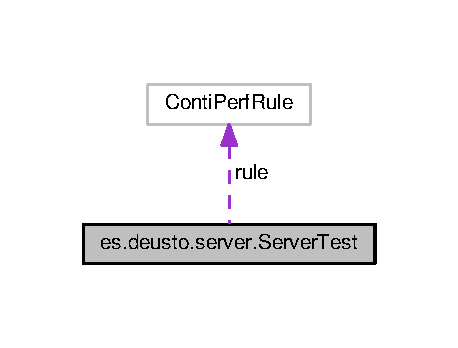
\includegraphics[width=220pt]{classes_1_1deusto_1_1server_1_1_server_test__coll__graph}
\end{center}
\end{figure}
\subsection*{Public Member Functions}
\begin{DoxyCompactItemize}
\item 
void \hyperlink{classes_1_1deusto_1_1server_1_1_server_test_af715b0b972d52aaa4d90bf086f990921}{set\+Up} ()
\item 
.junit.\+Test void \hyperlink{classes_1_1deusto_1_1server_1_1_server_test_a7c2dd5cf5eb68dbf35b10f6c29b6734f}{test\+Log\+In\+User} ()  throws Remote\+Exception, Interrupted\+Exception 
\item 
.junit.\+Test void \hyperlink{classes_1_1deusto_1_1server_1_1_server_test_ade2896be992e43bbfb29ba455da9d335}{test\+Log\+In\+Admin} ()  throws Remote\+Exception 
\item 
.junit.\+Test void \hyperlink{classes_1_1deusto_1_1server_1_1_server_test_adb4299be45a2652280186729967b6f78}{test\+Register} ()  throws Remote\+Exception, Interrupted\+Exception 
\item 
.junit.\+Test void \hyperlink{classes_1_1deusto_1_1server_1_1_server_test_ae9706506ea1913688180ef68f900c73a}{test\+Articles\+Management} ()  throws Remote\+Exception, Interrupted\+Exception 
\item 
.junit.\+Test void \hyperlink{classes_1_1deusto_1_1server_1_1_server_test_a3e97ef887212fc0047e556559d9677ba}{get\+First\+Articles} ()  throws Remote\+Exception, Interrupted\+Exception 
\end{DoxyCompactItemize}
\subsection*{Static Public Member Functions}
\begin{DoxyCompactItemize}
\item 
static junit.\+framework.\+Test \hyperlink{classes_1_1deusto_1_1server_1_1_server_test_a395162326c0f8b35291916b6427e697a}{suite} ()
\end{DoxyCompactItemize}
\subsection*{Public Attributes}
\begin{DoxyCompactItemize}
\item 
Conti\+Perf\+Rule \hyperlink{classes_1_1deusto_1_1server_1_1_server_test_ab2224d0a68cc9af1c1abded7e27f4241}{rule} = new Conti\+Perf\+Rule()
\end{DoxyCompactItemize}


\subsection{Detailed Description}
Unit test for the server part. 

Definition at line 47 of file Server\+Test.\+java.



\subsection{Member Function Documentation}
\mbox{\Hypertarget{classes_1_1deusto_1_1server_1_1_server_test_a3e97ef887212fc0047e556559d9677ba}\label{classes_1_1deusto_1_1server_1_1_server_test_a3e97ef887212fc0047e556559d9677ba}} 
\index{es\+::deusto\+::server\+::\+Server\+Test@{es\+::deusto\+::server\+::\+Server\+Test}!get\+First\+Articles@{get\+First\+Articles}}
\index{get\+First\+Articles@{get\+First\+Articles}!es\+::deusto\+::server\+::\+Server\+Test@{es\+::deusto\+::server\+::\+Server\+Test}}
\subsubsection{\texorpdfstring{get\+First\+Articles()}{getFirstArticles()}}
{\footnotesize\ttfamily .junit.\+Test void es.\+deusto.\+server.\+Server\+Test.\+get\+First\+Articles (\begin{DoxyParamCaption}{ }\end{DoxyParamCaption}) throws Remote\+Exception, Interrupted\+Exception}



Definition at line 126 of file Server\+Test.\+java.

\mbox{\Hypertarget{classes_1_1deusto_1_1server_1_1_server_test_af715b0b972d52aaa4d90bf086f990921}\label{classes_1_1deusto_1_1server_1_1_server_test_af715b0b972d52aaa4d90bf086f990921}} 
\index{es\+::deusto\+::server\+::\+Server\+Test@{es\+::deusto\+::server\+::\+Server\+Test}!set\+Up@{set\+Up}}
\index{set\+Up@{set\+Up}!es\+::deusto\+::server\+::\+Server\+Test@{es\+::deusto\+::server\+::\+Server\+Test}}
\subsubsection{\texorpdfstring{set\+Up()}{setUp()}}
{\footnotesize\ttfamily void es.\+deusto.\+server.\+Server\+Test.\+set\+Up (\begin{DoxyParamCaption}{ }\end{DoxyParamCaption})}



Definition at line 63 of file Server\+Test.\+java.

\mbox{\Hypertarget{classes_1_1deusto_1_1server_1_1_server_test_a395162326c0f8b35291916b6427e697a}\label{classes_1_1deusto_1_1server_1_1_server_test_a395162326c0f8b35291916b6427e697a}} 
\index{es\+::deusto\+::server\+::\+Server\+Test@{es\+::deusto\+::server\+::\+Server\+Test}!suite@{suite}}
\index{suite@{suite}!es\+::deusto\+::server\+::\+Server\+Test@{es\+::deusto\+::server\+::\+Server\+Test}}
\subsubsection{\texorpdfstring{suite()}{suite()}}
{\footnotesize\ttfamily static junit.\+framework.\+Test es.\+deusto.\+server.\+Server\+Test.\+suite (\begin{DoxyParamCaption}{ }\end{DoxyParamCaption})\hspace{0.3cm}{\ttfamily [static]}}

\begin{DoxyReturn}{Returns}
the suite of tests being tested 
\end{DoxyReturn}


Definition at line 58 of file Server\+Test.\+java.

\mbox{\Hypertarget{classes_1_1deusto_1_1server_1_1_server_test_ae9706506ea1913688180ef68f900c73a}\label{classes_1_1deusto_1_1server_1_1_server_test_ae9706506ea1913688180ef68f900c73a}} 
\index{es\+::deusto\+::server\+::\+Server\+Test@{es\+::deusto\+::server\+::\+Server\+Test}!test\+Articles\+Management@{test\+Articles\+Management}}
\index{test\+Articles\+Management@{test\+Articles\+Management}!es\+::deusto\+::server\+::\+Server\+Test@{es\+::deusto\+::server\+::\+Server\+Test}}
\subsubsection{\texorpdfstring{test\+Articles\+Management()}{testArticlesManagement()}}
{\footnotesize\ttfamily .junit.\+Test void es.\+deusto.\+server.\+Server\+Test.\+test\+Articles\+Management (\begin{DoxyParamCaption}{ }\end{DoxyParamCaption}) throws Remote\+Exception, Interrupted\+Exception}



Definition at line 101 of file Server\+Test.\+java.

\mbox{\Hypertarget{classes_1_1deusto_1_1server_1_1_server_test_ade2896be992e43bbfb29ba455da9d335}\label{classes_1_1deusto_1_1server_1_1_server_test_ade2896be992e43bbfb29ba455da9d335}} 
\index{es\+::deusto\+::server\+::\+Server\+Test@{es\+::deusto\+::server\+::\+Server\+Test}!test\+Log\+In\+Admin@{test\+Log\+In\+Admin}}
\index{test\+Log\+In\+Admin@{test\+Log\+In\+Admin}!es\+::deusto\+::server\+::\+Server\+Test@{es\+::deusto\+::server\+::\+Server\+Test}}
\subsubsection{\texorpdfstring{test\+Log\+In\+Admin()}{testLogInAdmin()}}
{\footnotesize\ttfamily .junit.\+Test void es.\+deusto.\+server.\+Server\+Test.\+test\+Log\+In\+Admin (\begin{DoxyParamCaption}{ }\end{DoxyParamCaption}) throws Remote\+Exception}



Definition at line 86 of file Server\+Test.\+java.

\mbox{\Hypertarget{classes_1_1deusto_1_1server_1_1_server_test_a7c2dd5cf5eb68dbf35b10f6c29b6734f}\label{classes_1_1deusto_1_1server_1_1_server_test_a7c2dd5cf5eb68dbf35b10f6c29b6734f}} 
\index{es\+::deusto\+::server\+::\+Server\+Test@{es\+::deusto\+::server\+::\+Server\+Test}!test\+Log\+In\+User@{test\+Log\+In\+User}}
\index{test\+Log\+In\+User@{test\+Log\+In\+User}!es\+::deusto\+::server\+::\+Server\+Test@{es\+::deusto\+::server\+::\+Server\+Test}}
\subsubsection{\texorpdfstring{test\+Log\+In\+User()}{testLogInUser()}}
{\footnotesize\ttfamily .junit.\+Test void es.\+deusto.\+server.\+Server\+Test.\+test\+Log\+In\+User (\begin{DoxyParamCaption}{ }\end{DoxyParamCaption}) throws Remote\+Exception, Interrupted\+Exception}



Definition at line 78 of file Server\+Test.\+java.

\mbox{\Hypertarget{classes_1_1deusto_1_1server_1_1_server_test_adb4299be45a2652280186729967b6f78}\label{classes_1_1deusto_1_1server_1_1_server_test_adb4299be45a2652280186729967b6f78}} 
\index{es\+::deusto\+::server\+::\+Server\+Test@{es\+::deusto\+::server\+::\+Server\+Test}!test\+Register@{test\+Register}}
\index{test\+Register@{test\+Register}!es\+::deusto\+::server\+::\+Server\+Test@{es\+::deusto\+::server\+::\+Server\+Test}}
\subsubsection{\texorpdfstring{test\+Register()}{testRegister()}}
{\footnotesize\ttfamily .junit.\+Test void es.\+deusto.\+server.\+Server\+Test.\+test\+Register (\begin{DoxyParamCaption}{ }\end{DoxyParamCaption}) throws Remote\+Exception, Interrupted\+Exception}



Definition at line 94 of file Server\+Test.\+java.



\subsection{Member Data Documentation}
\mbox{\Hypertarget{classes_1_1deusto_1_1server_1_1_server_test_ab2224d0a68cc9af1c1abded7e27f4241}\label{classes_1_1deusto_1_1server_1_1_server_test_ab2224d0a68cc9af1c1abded7e27f4241}} 
\index{es\+::deusto\+::server\+::\+Server\+Test@{es\+::deusto\+::server\+::\+Server\+Test}!rule@{rule}}
\index{rule@{rule}!es\+::deusto\+::server\+::\+Server\+Test@{es\+::deusto\+::server\+::\+Server\+Test}}
\subsubsection{\texorpdfstring{rule}{rule}}
{\footnotesize\ttfamily Conti\+Perf\+Rule es.\+deusto.\+server.\+Server\+Test.\+rule = new Conti\+Perf\+Rule()}



Definition at line 53 of file Server\+Test.\+java.



The documentation for this class was generated from the following file\+:\begin{DoxyCompactItemize}
\item 
/home/albertofdr/git/\+B\+S\+P\+Q19-\/\+E3/src/test/java/es/deusto/server/\hyperlink{_server_test_8java}{Server\+Test.\+java}\end{DoxyCompactItemize}

\hypertarget{classes_1_1deusto_1_1server_1_1jdo_1_1_user}{}\section{es.\+deusto.\+server.\+jdo.\+User Class Reference}
\label{classes_1_1deusto_1_1server_1_1jdo_1_1_user}\index{es.\+deusto.\+server.\+jdo.\+User@{es.\+deusto.\+server.\+jdo.\+User}}


Inheritance diagram for es.\+deusto.\+server.\+jdo.\+User\+:
\nopagebreak
\begin{figure}[H]
\begin{center}
\leavevmode
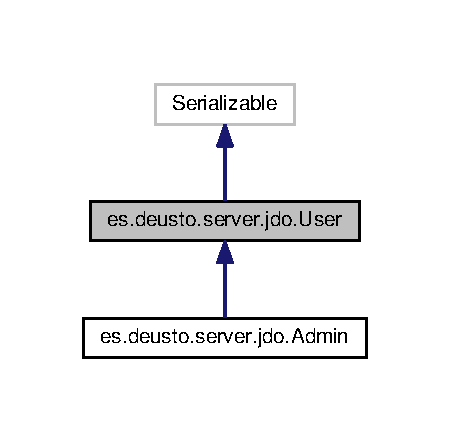
\includegraphics[width=216pt]{classes_1_1deusto_1_1server_1_1jdo_1_1_user__inherit__graph}
\end{center}
\end{figure}


Collaboration diagram for es.\+deusto.\+server.\+jdo.\+User\+:
\nopagebreak
\begin{figure}[H]
\begin{center}
\leavevmode
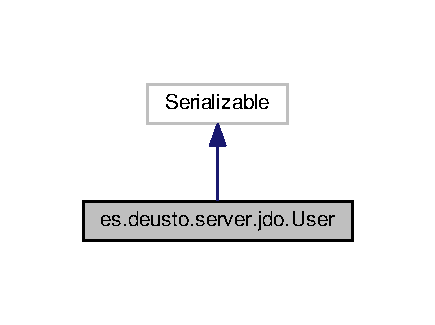
\includegraphics[width=209pt]{classes_1_1deusto_1_1server_1_1jdo_1_1_user__coll__graph}
\end{center}
\end{figure}
\subsection*{Public Member Functions}
\begin{DoxyCompactItemize}
\item 
\hyperlink{classes_1_1deusto_1_1server_1_1jdo_1_1_user_a9c791374ed16461ebae0ed38005a8b56}{User} (String \hyperlink{classes_1_1deusto_1_1server_1_1jdo_1_1_user_aa1f05a7b487224d7c846fb81e5262c00}{username}, String \hyperlink{classes_1_1deusto_1_1server_1_1jdo_1_1_user_a9e3d470b8d2b36996759bd0595984870}{password}, String \hyperlink{classes_1_1deusto_1_1server_1_1jdo_1_1_user_a2aedb628a946e5044f27a3e6cbda31f0}{email})
\item 
String \hyperlink{classes_1_1deusto_1_1server_1_1jdo_1_1_user_aad8107ea8f9281199377f705d541bf8e}{get\+Login} ()
\item 
String \hyperlink{classes_1_1deusto_1_1server_1_1jdo_1_1_user_a1900ee126da22ed0f043e0077e8be049}{get\+Password} ()
\item 
void \hyperlink{classes_1_1deusto_1_1server_1_1jdo_1_1_user_a50b19b7520eb089012413d6072c1b7a2}{set\+Username} (String user)
\item 
void \hyperlink{classes_1_1deusto_1_1server_1_1jdo_1_1_user_a2e052b5a7cab949f61580edf44bbd233}{set\+Password} (String \hyperlink{classes_1_1deusto_1_1server_1_1jdo_1_1_user_a9e3d470b8d2b36996759bd0595984870}{password})
\item 
String \hyperlink{classes_1_1deusto_1_1server_1_1jdo_1_1_user_aa1ba6d9e3d0572b90dac6ff627ee3f95}{get\+Email} ()
\item 
boolean \hyperlink{classes_1_1deusto_1_1server_1_1jdo_1_1_user_a6488131800327e3353fd785d2db06b16}{equals} (\hyperlink{classes_1_1deusto_1_1server_1_1jdo_1_1_user}{User} obj)
\item 
int \hyperlink{classes_1_1deusto_1_1server_1_1jdo_1_1_user_aeabfaac22221c47ca92d8a60376c742c}{hash\+Code} ()
\item 
String \hyperlink{classes_1_1deusto_1_1server_1_1jdo_1_1_user_a65366a578a6dcc53e3a77d6eabbbf8cf}{to\+String} ()
\end{DoxyCompactItemize}
\subsection*{Public Attributes}
\begin{DoxyCompactItemize}
\item 
String \hyperlink{classes_1_1deusto_1_1server_1_1jdo_1_1_user_aa1f05a7b487224d7c846fb81e5262c00}{username}
\item 
String \hyperlink{classes_1_1deusto_1_1server_1_1jdo_1_1_user_a9e3d470b8d2b36996759bd0595984870}{password}
\item 
String \hyperlink{classes_1_1deusto_1_1server_1_1jdo_1_1_user_a2aedb628a946e5044f27a3e6cbda31f0}{email}
\end{DoxyCompactItemize}
\subsection*{Protected Member Functions}
\begin{DoxyCompactItemize}
\item 
\hyperlink{classes_1_1deusto_1_1server_1_1jdo_1_1_user_a4d382337425fcc968d350709e15863b1}{User} ()
\end{DoxyCompactItemize}


\subsection{Detailed Description}
The class for the normal user. \begin{DoxyAuthor}{Author}
albertofdr 
\end{DoxyAuthor}


Definition at line 14 of file User.\+java.



\subsection{Constructor \& Destructor Documentation}
\mbox{\Hypertarget{classes_1_1deusto_1_1server_1_1jdo_1_1_user_a9c791374ed16461ebae0ed38005a8b56}\label{classes_1_1deusto_1_1server_1_1jdo_1_1_user_a9c791374ed16461ebae0ed38005a8b56}} 
\index{es\+::deusto\+::server\+::jdo\+::\+User@{es\+::deusto\+::server\+::jdo\+::\+User}!User@{User}}
\index{User@{User}!es\+::deusto\+::server\+::jdo\+::\+User@{es\+::deusto\+::server\+::jdo\+::\+User}}
\subsubsection{\texorpdfstring{User()}{User()}\hspace{0.1cm}{\footnotesize\ttfamily [1/2]}}
{\footnotesize\ttfamily es.\+deusto.\+server.\+jdo.\+User.\+User (\begin{DoxyParamCaption}\item[{String}]{username,  }\item[{String}]{password,  }\item[{String}]{email }\end{DoxyParamCaption})}


\begin{DoxyParams}{Parameters}
{\em username} & The name of the \hyperlink{classes_1_1deusto_1_1server_1_1jdo_1_1_user}{User} \\
\hline
{\em password} & The password that will use for login \\
\hline
{\em email} & The email of that person \\
\hline
\end{DoxyParams}


Definition at line 27 of file User.\+java.

\mbox{\Hypertarget{classes_1_1deusto_1_1server_1_1jdo_1_1_user_a4d382337425fcc968d350709e15863b1}\label{classes_1_1deusto_1_1server_1_1jdo_1_1_user_a4d382337425fcc968d350709e15863b1}} 
\index{es\+::deusto\+::server\+::jdo\+::\+User@{es\+::deusto\+::server\+::jdo\+::\+User}!User@{User}}
\index{User@{User}!es\+::deusto\+::server\+::jdo\+::\+User@{es\+::deusto\+::server\+::jdo\+::\+User}}
\subsubsection{\texorpdfstring{User()}{User()}\hspace{0.1cm}{\footnotesize\ttfamily [2/2]}}
{\footnotesize\ttfamily es.\+deusto.\+server.\+jdo.\+User.\+User (\begin{DoxyParamCaption}{ }\end{DoxyParamCaption})\hspace{0.3cm}{\ttfamily [protected]}}



Definition at line 33 of file User.\+java.



\subsection{Member Function Documentation}
\mbox{\Hypertarget{classes_1_1deusto_1_1server_1_1jdo_1_1_user_a6488131800327e3353fd785d2db06b16}\label{classes_1_1deusto_1_1server_1_1jdo_1_1_user_a6488131800327e3353fd785d2db06b16}} 
\index{es\+::deusto\+::server\+::jdo\+::\+User@{es\+::deusto\+::server\+::jdo\+::\+User}!equals@{equals}}
\index{equals@{equals}!es\+::deusto\+::server\+::jdo\+::\+User@{es\+::deusto\+::server\+::jdo\+::\+User}}
\subsubsection{\texorpdfstring{equals()}{equals()}}
{\footnotesize\ttfamily boolean es.\+deusto.\+server.\+jdo.\+User.\+equals (\begin{DoxyParamCaption}\item[{\hyperlink{classes_1_1deusto_1_1server_1_1jdo_1_1_user}{User}}]{obj }\end{DoxyParamCaption})}

Compare two users if they are the same 
\begin{DoxyParams}{Parameters}
{\em obj} & A user to compare \\
\hline
\end{DoxyParams}
\begin{DoxyReturn}{Returns}
Return if the two user are equals 
\end{DoxyReturn}


Definition at line 81 of file User.\+java.

\mbox{\Hypertarget{classes_1_1deusto_1_1server_1_1jdo_1_1_user_aa1ba6d9e3d0572b90dac6ff627ee3f95}\label{classes_1_1deusto_1_1server_1_1jdo_1_1_user_aa1ba6d9e3d0572b90dac6ff627ee3f95}} 
\index{es\+::deusto\+::server\+::jdo\+::\+User@{es\+::deusto\+::server\+::jdo\+::\+User}!get\+Email@{get\+Email}}
\index{get\+Email@{get\+Email}!es\+::deusto\+::server\+::jdo\+::\+User@{es\+::deusto\+::server\+::jdo\+::\+User}}
\subsubsection{\texorpdfstring{get\+Email()}{getEmail()}}
{\footnotesize\ttfamily String es.\+deusto.\+server.\+jdo.\+User.\+get\+Email (\begin{DoxyParamCaption}{ }\end{DoxyParamCaption})}

\begin{DoxyReturn}{Returns}
Set a new email for the user 
\end{DoxyReturn}


Definition at line 72 of file User.\+java.

\mbox{\Hypertarget{classes_1_1deusto_1_1server_1_1jdo_1_1_user_aad8107ea8f9281199377f705d541bf8e}\label{classes_1_1deusto_1_1server_1_1jdo_1_1_user_aad8107ea8f9281199377f705d541bf8e}} 
\index{es\+::deusto\+::server\+::jdo\+::\+User@{es\+::deusto\+::server\+::jdo\+::\+User}!get\+Login@{get\+Login}}
\index{get\+Login@{get\+Login}!es\+::deusto\+::server\+::jdo\+::\+User@{es\+::deusto\+::server\+::jdo\+::\+User}}
\subsubsection{\texorpdfstring{get\+Login()}{getLogin()}}
{\footnotesize\ttfamily String es.\+deusto.\+server.\+jdo.\+User.\+get\+Login (\begin{DoxyParamCaption}{ }\end{DoxyParamCaption})}

\begin{DoxyReturn}{Returns}
Gets you the username of this user 
\end{DoxyReturn}


Definition at line 39 of file User.\+java.

\mbox{\Hypertarget{classes_1_1deusto_1_1server_1_1jdo_1_1_user_a1900ee126da22ed0f043e0077e8be049}\label{classes_1_1deusto_1_1server_1_1jdo_1_1_user_a1900ee126da22ed0f043e0077e8be049}} 
\index{es\+::deusto\+::server\+::jdo\+::\+User@{es\+::deusto\+::server\+::jdo\+::\+User}!get\+Password@{get\+Password}}
\index{get\+Password@{get\+Password}!es\+::deusto\+::server\+::jdo\+::\+User@{es\+::deusto\+::server\+::jdo\+::\+User}}
\subsubsection{\texorpdfstring{get\+Password()}{getPassword()}}
{\footnotesize\ttfamily String es.\+deusto.\+server.\+jdo.\+User.\+get\+Password (\begin{DoxyParamCaption}{ }\end{DoxyParamCaption})}

\begin{DoxyReturn}{Returns}
Gets you the password of this user 
\end{DoxyReturn}


Definition at line 47 of file User.\+java.

\mbox{\Hypertarget{classes_1_1deusto_1_1server_1_1jdo_1_1_user_aeabfaac22221c47ca92d8a60376c742c}\label{classes_1_1deusto_1_1server_1_1jdo_1_1_user_aeabfaac22221c47ca92d8a60376c742c}} 
\index{es\+::deusto\+::server\+::jdo\+::\+User@{es\+::deusto\+::server\+::jdo\+::\+User}!hash\+Code@{hash\+Code}}
\index{hash\+Code@{hash\+Code}!es\+::deusto\+::server\+::jdo\+::\+User@{es\+::deusto\+::server\+::jdo\+::\+User}}
\subsubsection{\texorpdfstring{hash\+Code()}{hashCode()}}
{\footnotesize\ttfamily int es.\+deusto.\+server.\+jdo.\+User.\+hash\+Code (\begin{DoxyParamCaption}{ }\end{DoxyParamCaption})}

Hashcode for the user 

Definition at line 93 of file User.\+java.

\mbox{\Hypertarget{classes_1_1deusto_1_1server_1_1jdo_1_1_user_a2e052b5a7cab949f61580edf44bbd233}\label{classes_1_1deusto_1_1server_1_1jdo_1_1_user_a2e052b5a7cab949f61580edf44bbd233}} 
\index{es\+::deusto\+::server\+::jdo\+::\+User@{es\+::deusto\+::server\+::jdo\+::\+User}!set\+Password@{set\+Password}}
\index{set\+Password@{set\+Password}!es\+::deusto\+::server\+::jdo\+::\+User@{es\+::deusto\+::server\+::jdo\+::\+User}}
\subsubsection{\texorpdfstring{set\+Password()}{setPassword()}}
{\footnotesize\ttfamily void es.\+deusto.\+server.\+jdo.\+User.\+set\+Password (\begin{DoxyParamCaption}\item[{String}]{password }\end{DoxyParamCaption})}


\begin{DoxyParams}{Parameters}
{\em password} & Set a new password of the user \\
\hline
\end{DoxyParams}


Definition at line 64 of file User.\+java.

\mbox{\Hypertarget{classes_1_1deusto_1_1server_1_1jdo_1_1_user_a50b19b7520eb089012413d6072c1b7a2}\label{classes_1_1deusto_1_1server_1_1jdo_1_1_user_a50b19b7520eb089012413d6072c1b7a2}} 
\index{es\+::deusto\+::server\+::jdo\+::\+User@{es\+::deusto\+::server\+::jdo\+::\+User}!set\+Username@{set\+Username}}
\index{set\+Username@{set\+Username}!es\+::deusto\+::server\+::jdo\+::\+User@{es\+::deusto\+::server\+::jdo\+::\+User}}
\subsubsection{\texorpdfstring{set\+Username()}{setUsername()}}
{\footnotesize\ttfamily void es.\+deusto.\+server.\+jdo.\+User.\+set\+Username (\begin{DoxyParamCaption}\item[{String}]{user }\end{DoxyParamCaption})}


\begin{DoxyParams}{Parameters}
{\em user} & Set a new username of the user \\
\hline
\end{DoxyParams}


Definition at line 55 of file User.\+java.

\mbox{\Hypertarget{classes_1_1deusto_1_1server_1_1jdo_1_1_user_a65366a578a6dcc53e3a77d6eabbbf8cf}\label{classes_1_1deusto_1_1server_1_1jdo_1_1_user_a65366a578a6dcc53e3a77d6eabbbf8cf}} 
\index{es\+::deusto\+::server\+::jdo\+::\+User@{es\+::deusto\+::server\+::jdo\+::\+User}!to\+String@{to\+String}}
\index{to\+String@{to\+String}!es\+::deusto\+::server\+::jdo\+::\+User@{es\+::deusto\+::server\+::jdo\+::\+User}}
\subsubsection{\texorpdfstring{to\+String()}{toString()}}
{\footnotesize\ttfamily String es.\+deusto.\+server.\+jdo.\+User.\+to\+String (\begin{DoxyParamCaption}{ }\end{DoxyParamCaption})}

Method to print the user 

Definition at line 101 of file User.\+java.



\subsection{Member Data Documentation}
\mbox{\Hypertarget{classes_1_1deusto_1_1server_1_1jdo_1_1_user_a2aedb628a946e5044f27a3e6cbda31f0}\label{classes_1_1deusto_1_1server_1_1jdo_1_1_user_a2aedb628a946e5044f27a3e6cbda31f0}} 
\index{es\+::deusto\+::server\+::jdo\+::\+User@{es\+::deusto\+::server\+::jdo\+::\+User}!email@{email}}
\index{email@{email}!es\+::deusto\+::server\+::jdo\+::\+User@{es\+::deusto\+::server\+::jdo\+::\+User}}
\subsubsection{\texorpdfstring{email}{email}}
{\footnotesize\ttfamily String es.\+deusto.\+server.\+jdo.\+User.\+email}



Definition at line 19 of file User.\+java.

\mbox{\Hypertarget{classes_1_1deusto_1_1server_1_1jdo_1_1_user_a9e3d470b8d2b36996759bd0595984870}\label{classes_1_1deusto_1_1server_1_1jdo_1_1_user_a9e3d470b8d2b36996759bd0595984870}} 
\index{es\+::deusto\+::server\+::jdo\+::\+User@{es\+::deusto\+::server\+::jdo\+::\+User}!password@{password}}
\index{password@{password}!es\+::deusto\+::server\+::jdo\+::\+User@{es\+::deusto\+::server\+::jdo\+::\+User}}
\subsubsection{\texorpdfstring{password}{password}}
{\footnotesize\ttfamily String es.\+deusto.\+server.\+jdo.\+User.\+password}



Definition at line 18 of file User.\+java.

\mbox{\Hypertarget{classes_1_1deusto_1_1server_1_1jdo_1_1_user_aa1f05a7b487224d7c846fb81e5262c00}\label{classes_1_1deusto_1_1server_1_1jdo_1_1_user_aa1f05a7b487224d7c846fb81e5262c00}} 
\index{es\+::deusto\+::server\+::jdo\+::\+User@{es\+::deusto\+::server\+::jdo\+::\+User}!username@{username}}
\index{username@{username}!es\+::deusto\+::server\+::jdo\+::\+User@{es\+::deusto\+::server\+::jdo\+::\+User}}
\subsubsection{\texorpdfstring{username}{username}}
{\footnotesize\ttfamily String es.\+deusto.\+server.\+jdo.\+User.\+username}



Definition at line 17 of file User.\+java.



The documentation for this class was generated from the following file\+:\begin{DoxyCompactItemize}
\item 
src/main/java/es/deusto/server/jdo/\hyperlink{_user_8java}{User.\+java}\end{DoxyCompactItemize}

\hypertarget{classes_1_1deusto_1_1server_1_1jdo_1_1_user_test}{}\section{es.\+deusto.\+server.\+jdo.\+User\+Test Class Reference}
\label{classes_1_1deusto_1_1server_1_1jdo_1_1_user_test}\index{es.\+deusto.\+server.\+jdo.\+User\+Test@{es.\+deusto.\+server.\+jdo.\+User\+Test}}
\subsection*{Public Member Functions}
\begin{DoxyCompactItemize}
\item 
void \hyperlink{classes_1_1deusto_1_1server_1_1jdo_1_1_user_test_a00292ba5127aa4a2c2b31514c3a929ed}{User\+Test} ()
\item 
.junit.\+Test void \hyperlink{classes_1_1deusto_1_1server_1_1jdo_1_1_user_test_aec9f7ccc079890364b8270d8645e6957}{test\+App} ()
\end{DoxyCompactItemize}
\subsection*{Static Public Member Functions}
\begin{DoxyCompactItemize}
\item 
static junit.\+framework.\+Test \hyperlink{classes_1_1deusto_1_1server_1_1jdo_1_1_user_test_af4c617a2b9b0593aaaf7d21373190401}{suite} ()
\end{DoxyCompactItemize}


\subsection{Detailed Description}


Definition at line 14 of file User\+Test.\+java.



\subsection{Constructor \& Destructor Documentation}
\mbox{\Hypertarget{classes_1_1deusto_1_1server_1_1jdo_1_1_user_test_a00292ba5127aa4a2c2b31514c3a929ed}\label{classes_1_1deusto_1_1server_1_1jdo_1_1_user_test_a00292ba5127aa4a2c2b31514c3a929ed}} 
\index{es\+::deusto\+::server\+::jdo\+::\+User\+Test@{es\+::deusto\+::server\+::jdo\+::\+User\+Test}!User\+Test@{User\+Test}}
\index{User\+Test@{User\+Test}!es\+::deusto\+::server\+::jdo\+::\+User\+Test@{es\+::deusto\+::server\+::jdo\+::\+User\+Test}}
\subsubsection{\texorpdfstring{User\+Test()}{UserTest()}}
{\footnotesize\ttfamily void es.\+deusto.\+server.\+jdo.\+User\+Test.\+User\+Test (\begin{DoxyParamCaption}{ }\end{DoxyParamCaption})}

Create the test case


\begin{DoxyParams}{Parameters}
{\em test\+Name} & name of the test case \\
\hline
\end{DoxyParams}


Definition at line 33 of file User\+Test.\+java.



\subsection{Member Function Documentation}
\mbox{\Hypertarget{classes_1_1deusto_1_1server_1_1jdo_1_1_user_test_af4c617a2b9b0593aaaf7d21373190401}\label{classes_1_1deusto_1_1server_1_1jdo_1_1_user_test_af4c617a2b9b0593aaaf7d21373190401}} 
\index{es\+::deusto\+::server\+::jdo\+::\+User\+Test@{es\+::deusto\+::server\+::jdo\+::\+User\+Test}!suite@{suite}}
\index{suite@{suite}!es\+::deusto\+::server\+::jdo\+::\+User\+Test@{es\+::deusto\+::server\+::jdo\+::\+User\+Test}}
\subsubsection{\texorpdfstring{suite()}{suite()}}
{\footnotesize\ttfamily static junit.\+framework.\+Test es.\+deusto.\+server.\+jdo.\+User\+Test.\+suite (\begin{DoxyParamCaption}{ }\end{DoxyParamCaption})\hspace{0.3cm}{\ttfamily [static]}}

\begin{DoxyReturn}{Returns}
the suite of tests being tested 
\end{DoxyReturn}


Definition at line 24 of file User\+Test.\+java.

\mbox{\Hypertarget{classes_1_1deusto_1_1server_1_1jdo_1_1_user_test_aec9f7ccc079890364b8270d8645e6957}\label{classes_1_1deusto_1_1server_1_1jdo_1_1_user_test_aec9f7ccc079890364b8270d8645e6957}} 
\index{es\+::deusto\+::server\+::jdo\+::\+User\+Test@{es\+::deusto\+::server\+::jdo\+::\+User\+Test}!test\+App@{test\+App}}
\index{test\+App@{test\+App}!es\+::deusto\+::server\+::jdo\+::\+User\+Test@{es\+::deusto\+::server\+::jdo\+::\+User\+Test}}
\subsubsection{\texorpdfstring{test\+App()}{testApp()}}
{\footnotesize\ttfamily .junit.\+Test void es.\+deusto.\+server.\+jdo.\+User\+Test.\+test\+App (\begin{DoxyParamCaption}{ }\end{DoxyParamCaption})}

Test of the data 

Definition at line 45 of file User\+Test.\+java.



The documentation for this class was generated from the following file\+:\begin{DoxyCompactItemize}
\item 
src/test/java/es/deusto/server/jdo/\hyperlink{_user_test_8java}{User\+Test.\+java}\end{DoxyCompactItemize}

\chapter{File Documentation}
\hypertarget{_client_8java}{}\section{/home/albertofdr/git/\+B\+S\+P\+Q19-\/\+E3/src/main/java/es/deusto/client/\+Client.java File Reference}
\label{_client_8java}\index{/home/albertofdr/git/\+B\+S\+P\+Q19-\/\+E3/src/main/java/es/deusto/client/\+Client.\+java@{/home/albertofdr/git/\+B\+S\+P\+Q19-\/\+E3/src/main/java/es/deusto/client/\+Client.\+java}}
\subsection*{Classes}
\begin{DoxyCompactItemize}
\item 
class \hyperlink{classes_1_1deusto_1_1client_1_1_client}{es.\+deusto.\+client.\+Client}
\end{DoxyCompactItemize}
\subsection*{Packages}
\begin{DoxyCompactItemize}
\item 
package \hyperlink{namespacees_1_1deusto_1_1client}{es.\+deusto.\+client}
\begin{DoxyCompactList}\small\item\em This is the brief documentation for the Java package \hyperlink{namespacees_1_1deusto_1_1client}{es.\+deusto.\+client} which is a package for the client logic. \end{DoxyCompactList}\end{DoxyCompactItemize}

\hypertarget{_article_window_8java}{}\section{/home/albertofdr/git/\+B\+S\+P\+Q19-\/\+E3/src/main/java/es/deusto/client/\+G\+U\+I/\+Article\+Window.java File Reference}
\label{_article_window_8java}\index{/home/albertofdr/git/\+B\+S\+P\+Q19-\/\+E3/src/main/java/es/deusto/client/\+G\+U\+I/\+Article\+Window.\+java@{/home/albertofdr/git/\+B\+S\+P\+Q19-\/\+E3/src/main/java/es/deusto/client/\+G\+U\+I/\+Article\+Window.\+java}}
\subsection*{Classes}
\begin{DoxyCompactItemize}
\item 
class \hyperlink{classes_1_1deusto_1_1client_1_1_g_u_i_1_1_article_window}{es.\+deusto.\+client.\+G\+U\+I.\+Article\+Window}
\end{DoxyCompactItemize}
\subsection*{Packages}
\begin{DoxyCompactItemize}
\item 
package \hyperlink{namespacees_1_1deusto_1_1client_1_1_g_u_i}{es.\+deusto.\+client.\+G\+UI}
\begin{DoxyCompactList}\small\item\em This is the brief documentation for the Java package \hyperlink{namespacees_1_1deusto_1_1client_1_1_g_u_i}{es.\+deusto.\+client.\+G\+UI} which is a package for the client \hyperlink{namespacees_1_1deusto_1_1client_1_1_g_u_i}{G\+UI}. \end{DoxyCompactList}\end{DoxyCompactItemize}

\hypertarget{_login_window_user_8java}{}\section{/home/albertofdr/git/\+B\+S\+P\+Q19-\/\+E3/src/main/java/es/deusto/client/\+G\+U\+I/\+Login\+Window\+User.java File Reference}
\label{_login_window_user_8java}\index{/home/albertofdr/git/\+B\+S\+P\+Q19-\/\+E3/src/main/java/es/deusto/client/\+G\+U\+I/\+Login\+Window\+User.\+java@{/home/albertofdr/git/\+B\+S\+P\+Q19-\/\+E3/src/main/java/es/deusto/client/\+G\+U\+I/\+Login\+Window\+User.\+java}}
\subsection*{Classes}
\begin{DoxyCompactItemize}
\item 
class \hyperlink{classes_1_1deusto_1_1client_1_1_g_u_i_1_1_login_window_user}{es.\+deusto.\+client.\+G\+U\+I.\+Login\+Window\+User}
\end{DoxyCompactItemize}
\subsection*{Packages}
\begin{DoxyCompactItemize}
\item 
package \hyperlink{namespacees_1_1deusto_1_1client_1_1_g_u_i}{es.\+deusto.\+client.\+G\+UI}
\begin{DoxyCompactList}\small\item\em This is the brief documentation for the Java package \hyperlink{namespacees_1_1deusto_1_1client_1_1_g_u_i}{es.\+deusto.\+client.\+G\+UI} which is a package for the client \hyperlink{namespacees_1_1deusto_1_1client_1_1_g_u_i}{G\+UI}. \end{DoxyCompactList}\end{DoxyCompactItemize}

\hypertarget{_main_window_8java}{}\section{/home/albertofdr/git/\+B\+S\+P\+Q19-\/\+E3/src/main/java/es/deusto/client/\+G\+U\+I/\+Main\+Window.java File Reference}
\label{_main_window_8java}\index{/home/albertofdr/git/\+B\+S\+P\+Q19-\/\+E3/src/main/java/es/deusto/client/\+G\+U\+I/\+Main\+Window.\+java@{/home/albertofdr/git/\+B\+S\+P\+Q19-\/\+E3/src/main/java/es/deusto/client/\+G\+U\+I/\+Main\+Window.\+java}}
\subsection*{Classes}
\begin{DoxyCompactItemize}
\item 
class \hyperlink{classes_1_1deusto_1_1client_1_1_g_u_i_1_1_main_window}{es.\+deusto.\+client.\+G\+U\+I.\+Main\+Window}
\end{DoxyCompactItemize}
\subsection*{Packages}
\begin{DoxyCompactItemize}
\item 
package \hyperlink{namespacees_1_1deusto_1_1client_1_1_g_u_i}{es.\+deusto.\+client.\+G\+UI}
\begin{DoxyCompactList}\small\item\em This is the brief documentation for the Java package \hyperlink{namespacees_1_1deusto_1_1client_1_1_g_u_i}{es.\+deusto.\+client.\+G\+UI} which is a package for the client \hyperlink{namespacees_1_1deusto_1_1client_1_1_g_u_i}{G\+UI}. \end{DoxyCompactList}\end{DoxyCompactItemize}

\hypertarget{_i_server_8java}{}\section{src/main/java/es/deusto/server/\+I\+Server.java File Reference}
\label{_i_server_8java}\index{src/main/java/es/deusto/server/\+I\+Server.\+java@{src/main/java/es/deusto/server/\+I\+Server.\+java}}
\subsection*{Classes}
\begin{DoxyCompactItemize}
\item 
interface \hyperlink{interfacees_1_1deusto_1_1server_1_1_i_server}{es.\+deusto.\+server.\+I\+Server}
\end{DoxyCompactItemize}
\subsection*{Packages}
\begin{DoxyCompactItemize}
\item 
package \hyperlink{namespacees_1_1deusto_1_1server}{es.\+deusto.\+server}
\end{DoxyCompactItemize}

\hypertarget{_admin_8java}{}\section{src/main/java/es/deusto/server/jdo/\+Admin.java File Reference}
\label{_admin_8java}\index{src/main/java/es/deusto/server/jdo/\+Admin.\+java@{src/main/java/es/deusto/server/jdo/\+Admin.\+java}}
\subsection*{Classes}
\begin{DoxyCompactItemize}
\item 
class \hyperlink{classes_1_1deusto_1_1server_1_1jdo_1_1_admin}{es.\+deusto.\+server.\+jdo.\+Admin}
\end{DoxyCompactItemize}
\subsection*{Packages}
\begin{DoxyCompactItemize}
\item 
package \hyperlink{namespacees_1_1deusto_1_1server_1_1jdo}{es.\+deusto.\+server.\+jdo}
\end{DoxyCompactItemize}

\hypertarget{_article_8java}{}\section{/home/albertofdr/git/\+B\+S\+P\+Q19-\/\+E3/src/main/java/es/deusto/server/jdo/\+Article.java File Reference}
\label{_article_8java}\index{/home/albertofdr/git/\+B\+S\+P\+Q19-\/\+E3/src/main/java/es/deusto/server/jdo/\+Article.\+java@{/home/albertofdr/git/\+B\+S\+P\+Q19-\/\+E3/src/main/java/es/deusto/server/jdo/\+Article.\+java}}
\subsection*{Classes}
\begin{DoxyCompactItemize}
\item 
class \hyperlink{classes_1_1deusto_1_1server_1_1jdo_1_1_article}{es.\+deusto.\+server.\+jdo.\+Article}
\end{DoxyCompactItemize}
\subsection*{Packages}
\begin{DoxyCompactItemize}
\item 
package \hyperlink{namespacees_1_1deusto_1_1server_1_1jdo}{es.\+deusto.\+server.\+jdo}
\end{DoxyCompactItemize}

\hypertarget{_d_b_test_8java}{}\section{src/main/java/es/deusto/server/jdo/\+D\+B\+Test.java File Reference}
\label{_d_b_test_8java}\index{src/main/java/es/deusto/server/jdo/\+D\+B\+Test.\+java@{src/main/java/es/deusto/server/jdo/\+D\+B\+Test.\+java}}
\subsection*{Classes}
\begin{DoxyCompactItemize}
\item 
class \hyperlink{classes_1_1deusto_1_1server_1_1jdo_1_1_d_b_test}{es.\+deusto.\+server.\+jdo.\+D\+B\+Test}
\end{DoxyCompactItemize}
\subsection*{Packages}
\begin{DoxyCompactItemize}
\item 
package \hyperlink{namespacees_1_1deusto_1_1server_1_1jdo}{es.\+deusto.\+server.\+jdo}
\end{DoxyCompactItemize}

\hypertarget{_user_8java}{}\section{src/main/java/es/deusto/server/jdo/\+User.java File Reference}
\label{_user_8java}\index{src/main/java/es/deusto/server/jdo/\+User.\+java@{src/main/java/es/deusto/server/jdo/\+User.\+java}}
\subsection*{Classes}
\begin{DoxyCompactItemize}
\item 
class \hyperlink{classes_1_1deusto_1_1server_1_1jdo_1_1_user}{es.\+deusto.\+server.\+jdo.\+User}
\end{DoxyCompactItemize}
\subsection*{Packages}
\begin{DoxyCompactItemize}
\item 
package \hyperlink{namespacees_1_1deusto_1_1server_1_1jdo}{es.\+deusto.\+server.\+jdo}
\end{DoxyCompactItemize}

\hypertarget{_server_8java}{}\section{src/main/java/es/deusto/server/\+Server.java File Reference}
\label{_server_8java}\index{src/main/java/es/deusto/server/\+Server.\+java@{src/main/java/es/deusto/server/\+Server.\+java}}
\subsection*{Classes}
\begin{DoxyCompactItemize}
\item 
class \hyperlink{classes_1_1deusto_1_1server_1_1_server}{es.\+deusto.\+server.\+Server}
\end{DoxyCompactItemize}
\subsection*{Packages}
\begin{DoxyCompactItemize}
\item 
package \hyperlink{namespacees_1_1deusto_1_1server}{es.\+deusto.\+server}
\end{DoxyCompactItemize}

\hypertarget{_client_test_8java}{}\section{src/test/java/es/deusto/client/\+Client\+Test.java File Reference}
\label{_client_test_8java}\index{src/test/java/es/deusto/client/\+Client\+Test.\+java@{src/test/java/es/deusto/client/\+Client\+Test.\+java}}
\subsection*{Classes}
\begin{DoxyCompactItemize}
\item 
class \hyperlink{classes_1_1deusto_1_1client_1_1_client_test}{es.\+deusto.\+client.\+Client\+Test}
\end{DoxyCompactItemize}
\subsection*{Packages}
\begin{DoxyCompactItemize}
\item 
package \hyperlink{namespacees_1_1deusto_1_1client}{es.\+deusto.\+client}
\end{DoxyCompactItemize}

\hypertarget{_admin_test_8java}{}\section{src/test/java/es/deusto/server/jdo/\+Admin\+Test.java File Reference}
\label{_admin_test_8java}\index{src/test/java/es/deusto/server/jdo/\+Admin\+Test.\+java@{src/test/java/es/deusto/server/jdo/\+Admin\+Test.\+java}}
\subsection*{Classes}
\begin{DoxyCompactItemize}
\item 
class \hyperlink{classes_1_1deusto_1_1server_1_1jdo_1_1_admin_test}{es.\+deusto.\+server.\+jdo.\+Admin\+Test}
\end{DoxyCompactItemize}
\subsection*{Packages}
\begin{DoxyCompactItemize}
\item 
package \hyperlink{namespacees_1_1deusto_1_1server_1_1jdo}{es.\+deusto.\+server.\+jdo}
\end{DoxyCompactItemize}

\hypertarget{_article_test_8java}{}\section{src/test/java/es/deusto/server/jdo/\+Article\+Test.java File Reference}
\label{_article_test_8java}\index{src/test/java/es/deusto/server/jdo/\+Article\+Test.\+java@{src/test/java/es/deusto/server/jdo/\+Article\+Test.\+java}}
\subsection*{Classes}
\begin{DoxyCompactItemize}
\item 
class \hyperlink{classes_1_1deusto_1_1server_1_1jdo_1_1_article_test}{es.\+deusto.\+server.\+jdo.\+Article\+Test}
\end{DoxyCompactItemize}
\subsection*{Packages}
\begin{DoxyCompactItemize}
\item 
package \hyperlink{namespacees_1_1deusto_1_1server_1_1jdo}{es.\+deusto.\+server.\+jdo}
\end{DoxyCompactItemize}

\hypertarget{_user_test_8java}{}\section{/home/albertofdr/git/\+B\+S\+P\+Q19-\/\+E3/src/test/java/es/deusto/server/jdo/\+User\+Test.java File Reference}
\label{_user_test_8java}\index{/home/albertofdr/git/\+B\+S\+P\+Q19-\/\+E3/src/test/java/es/deusto/server/jdo/\+User\+Test.\+java@{/home/albertofdr/git/\+B\+S\+P\+Q19-\/\+E3/src/test/java/es/deusto/server/jdo/\+User\+Test.\+java}}
\subsection*{Classes}
\begin{DoxyCompactItemize}
\item 
class \hyperlink{classes_1_1deusto_1_1server_1_1jdo_1_1_user_test}{es.\+deusto.\+server.\+jdo.\+User\+Test}
\end{DoxyCompactItemize}
\subsection*{Packages}
\begin{DoxyCompactItemize}
\item 
package \hyperlink{namespacees_1_1deusto_1_1server_1_1jdo}{es.\+deusto.\+server.\+jdo}
\end{DoxyCompactItemize}

\hypertarget{_server_test_8java}{}\section{src/test/java/es/deusto/server/\+Server\+Test.java File Reference}
\label{_server_test_8java}\index{src/test/java/es/deusto/server/\+Server\+Test.\+java@{src/test/java/es/deusto/server/\+Server\+Test.\+java}}
\subsection*{Classes}
\begin{DoxyCompactItemize}
\item 
class \hyperlink{classes_1_1deusto_1_1server_1_1_server_test}{es.\+deusto.\+server.\+Server\+Test}
\end{DoxyCompactItemize}
\subsection*{Packages}
\begin{DoxyCompactItemize}
\item 
package \hyperlink{namespacees_1_1deusto_1_1server}{es.\+deusto.\+server}
\end{DoxyCompactItemize}

\hypertarget{_r_m_i_test_8java}{}\section{/home/albertofdr/git/\+B\+S\+P\+Q19-\/\+E3/src/test/java/\+R\+M\+I\+Test.java File Reference}
\label{_r_m_i_test_8java}\index{/home/albertofdr/git/\+B\+S\+P\+Q19-\/\+E3/src/test/java/\+R\+M\+I\+Test.\+java@{/home/albertofdr/git/\+B\+S\+P\+Q19-\/\+E3/src/test/java/\+R\+M\+I\+Test.\+java}}

%--- End generated contents ---

% Index
\backmatter
\newpage
\phantomsection
\clearemptydoublepage
\addcontentsline{toc}{chapter}{Index}
\printindex

\end{document}
